% ============================================================
% Capítulo VI — Doble refracción (§§144-197)
% Traducción de "Théorie mathématique de la lumière" (1889), cap. VI
% Original: §§144-197, páginas impresas 217-318
% Traducido en varias partes secuenciales; la Parte A cubre §§144-156
% (transformación de las ecuaciones, elipsoide de polarización y
% teoría de Fresnel), y las siguientes continúan desde el §157.
% ============================================================
\chapter{Doble refracción}
\label{cap:doble-refraccion}

\noindent\textbf{144.} El fenómeno de la doble refracción, observado por
primera vez hacia mediados del siglo~\textsc{xvii} en el espato de
Islandia, fue reconocido después en todas las sustancias cristalizadas que
no pertenecen al sistema cúbico. Biot, que estudió muy particularmente la
doble refracción desde el punto de vista experimental, dividió los
cristales birrefringentes en dos clases, según que los fenómenos fueran
simétricos alrededor de una recta o que parecieran coordinarse respecto de
dos rectas. Los cristales del primer grupo (\emph{cristales uniaxes})
pertenecen a uno de los sistemas cristalinos romboédrico, hexagonal o
cuadrático, que poseen un eje de simetría cristalográfica de orden
superior a~$2$; este eje de simetría se confunde con el eje \emph{óptico}
del cristal. Los cristales del segundo grupo (\emph{cristales biaxes}) son
ortorrómbicos, clinorrómbicos o anórticos; las direcciones de sus ejes
ópticos no están en relación inmediata con los elementos de simetría del
edificio cristalino. Fue Haüy el primero que hizo notar estas importantes
relaciones entre la forma cristalina y la propiedad birrefringente.

Las primeras investigaciones teóricas emprendidas con el fin de
explicar la marcha de la luz en los medios birrefringentes se deben a
Huygens; no se aplicaban más que a los cristales uniaxes. Fueron retomadas
por Young, pero este último, como tampoco Huygens, no llegó a una
verdadera explicación del fenómeno. A Fresnel le estaba reservada la gloria de hallar
la explicación matemática de las leyes de la doble refracción en los
cristales uniaxes y biaxes.

Los trabajos de Fresnel abrieron una vía nueva a las investigaciones de los
matemáticos. Cauchy, Lamé, Neumann, Mac-Cullagh y, muy recientemente,
MM.~Sarrau y Boussinesq, partiendo de consideraciones diferentes,
edificaron cierto número de teorías nuevas.

Estudiaremos sucesivamente estas diversas teorías. Antes, deduciremos de las
ecuaciones de los pequeños movimientos en un medio elástico la existencia
de una superficie de segundo grado que desempeña un papel capital en este
estudio y cuya introducción en la ciencia se debe a Cauchy; queremos hablar
del \emph{elipsoide de polarización}.

\section{Transformación de las ecuaciones del movimiento}

\noindent\textbf{145. Transformación de las ecuaciones del movimiento.} —
Mediante una elección conveniente de la unidad de masa, la densidad $\rho$
de una molécula de un medio elástico puede hacerse igual a $1$. En estas
condiciones, las ecuaciones generales del movimiento establecidas en el
§32 se convierten en
\begin{gather}
\frac{d^2\xi}{dt^2}=-\sum\frac{d}{dx}\cdot\frac{d\mathrm{W}_2}{d\xi'_x},\notag\\
\frac{d^2\eta}{dt^2}=-\sum\frac{d}{dx}\cdot\frac{d\mathrm{W}_2}{d\eta'_x},\notag\\
\frac{d^2\zeta}{dt^2}=-\sum\frac{d}{dx}\cdot\frac{d\mathrm{W}_2}{d\zeta'_x}.
\tag{1}
\end{gather}

Busquemos satisfacer estas ecuaciones mediante valores de $\xi,\eta,\zeta$
de la forma
\begin{equation}
\xi=A e^{P},\qquad \eta=Be^{P},\qquad \zeta=Ce^{P},
\tag{2}
\end{equation}
donde se tiene
\[
P=\frac{2i\pi}{\lambda}(\alpha x+\beta y+\gamma z - Vt).
\]
Tendremos así un movimiento que se propaga por ondas planas normales a la
recta que tiene por cosenos directores $\alpha,\beta,\gamma$. Reemplazando
en las ecuaciones del movimiento las derivadas parciales de
$\xi,\eta,\zeta$ por sus valores tomados de las igualdades (2),
obtendremos tres ecuaciones de condición entre las cantidades $A,B,C$ y la
velocidad de propagación $V$ del movimiento. Es posible dar a estas
ecuaciones una forma simple.

Las derivadas parciales de primer orden de $\xi,\eta,\zeta$ respecto de
las coordenadas $x,y,z$ contienen todas en factor la cantidad
$\frac{2i\pi}{\lambda}e^{P}$. Así, se tiene
\[
\xi'_x=\frac{2i\pi}{\lambda}\,\alpha A e^{P},\qquad
\xi'_y=\frac{2i\pi}{\lambda}\,\beta A e^{P},\ \ldots
\]
Por consiguiente $\mathrm{W}_2$, que es una función homogénea de segundo grado de
estas derivadas parciales, contendrá en factor
$\left(\frac{2i\pi}{\lambda}\right)^2 e^{2P}$. Si entonces ponemos
\[
\mathrm{W}_2=-\frac{1}{2}\left(\frac{2i\pi}{\lambda}\right)^2 e^{2P}\Pi,
\]
$\Pi$ será un polinomio homogéneo y de segundo grado respecto de $A,B,C$ y
respecto de $\alpha,\beta,\gamma$.

Derivando respecto de $A$ esta función $\mathrm{W}_2$, obtendremos
\begin{equation}
\frac{d\mathrm{W}_2}{dA}=-\frac{1}{2}\left(\frac{2i\pi}{\lambda}\right)^2 e^{2P}\frac{d\Pi}{dA}.
\tag{3}
\end{equation}
Por lo demás, la derivada de $\mathrm{W}_2$ respecto de $A$ puede escribirse
\[
\frac{d\mathrm{W}_2}{dA}=\sum\frac{d\mathrm{W}_2}{d\xi'_x}\cdot\frac{d\xi'_x}{dA};
\]
y, reemplazando en esta expresión las derivadas respecto de $A$ de las
diversas derivadas parciales de $\xi,\eta,\zeta$ por sus valores, tendremos
\[
\frac{d\mathrm{W}_2}{dA}=\frac{2i\pi}{\lambda}\,e^{P}\sum\alpha\,\frac{d\mathrm{W}_2}{d\xi'_x}.
\]
Igualando este valor de $\dfrac{d\mathrm{W}_2}{dA}$ al valor (3), y suprimiendo el
factor $\frac{2i\pi}{\lambda}e^{P}$ común a los dos miembros de la
igualdad obtenida, quedará
\begin{equation}
\sum\alpha\,\frac{d\mathrm{W}_2}{d\xi'_x}=-\frac{1}{2}\,\frac{2i\pi}{\lambda}\,e^{P}\,\frac{d\Pi}{dA}.
\tag{4}
\end{equation}

De esta igualdad vamos a deducir una nueva expresión del segundo miembro
de las ecuaciones (1) del movimiento. La derivada $\dfrac{d\mathrm{W}_2}{d\xi'_x}$
es una función homogénea y lineal respecto de las derivadas parciales de
las $\xi$; si entonces reemplazamos ahí estas derivadas parciales por sus
valores tomados de las relaciones (2), tendremos en factor la cantidad
$\frac{2i\pi}{\lambda}e^{P}$. Podemos entonces poner
\[
\frac{d\mathrm{W}_2}{d\xi'_x}=\frac{2i\pi}{\lambda}\,e^{P}\,\varphi,
\]
siendo $\varphi$ una función homogénea y lineal respecto de $A,B,C$ y de
$\alpha,\beta,\gamma$, pero sin depender de $x,y,z$. Por consiguiente
tendremos
\[
\frac{d}{dx}\cdot\frac{d\mathrm{W}_2}{d\xi'_x}=\frac{2i\pi}{\lambda}\,e^{P}\varphi\times\frac{dP}{dx}
=\frac{2i\pi}{\lambda}\,e^{P}\varphi\times\frac{2i\pi\alpha}{\lambda},
\]
o bien
\[
\frac{d}{dx}\cdot\frac{d\mathrm{W}_2}{d\xi'_x}=\frac{2i\pi}{\lambda}\,\alpha\,\frac{d\mathrm{W}_2}{d\xi'_x};
\]
y por consiguiente
\[
\sum\frac{d}{dx}\cdot\frac{d\mathrm{W}_2}{d\xi'_x}=\frac{2i\pi}{\lambda}\sum\alpha\,\frac{d\mathrm{W}_2}{d\xi'_x}.
\]
Reemplazando en el segundo miembro de esta expresión la cantidad colocada
bajo el signo $\sum$ por su valor (4), obtenemos
\[
\sum\frac{d}{dx}\cdot\frac{d\mathrm{W}_2}{d\xi'_x}=-\frac{1}{2}\left(\frac{2i\pi}{\lambda}\right)^2 e^{P}\,\frac{d\Pi}{dA};
\]
esto es, salvo el signo, el valor del segundo miembro de la primera de las
ecuaciones (1). Por otro lado, la primera de las igualdades (2) nos da
\[
\frac{d^2\xi}{dt^2}=Ae^{P}V^2\left(\frac{2i\pi}{\lambda}\right)^2;
\]
por consiguiente la primera de las ecuaciones del movimiento conduce a la
ecuación
\[
Ae^{P}V^2\left(\frac{2i\pi}{\lambda}\right)^2=\frac{1}{2}\left(\frac{2i\pi}{\lambda}\right)^2 e^{P}\,\frac{d\Pi}{dA},
\]
o,
\[
AV^2=\frac{1}{2}\,\frac{d\Pi}{dA}.
\]
Las otras dos ecuaciones del movimiento nos darían ecuaciones análogas;
por consiguiente las ecuaciones (1) pueden ser reemplazadas por el grupo
\begin{equation}
AV^2=\frac{1}{2}\frac{d\Pi}{dA},\qquad
BV^2=\frac{1}{2}\frac{d\Pi}{dB},\qquad
CV^2=\frac{1}{2}\frac{d\Pi}{dC}.
\tag{5}
\end{equation}

Se podría resolver analíticamente el sistema de las tres ecuaciones
precedentes; se obtendrían los valores de $V$ y de $A,B,C$ que, para
valores dados de $\alpha,\beta,\gamma$, dan desplazamientos $\xi,\eta,\zeta$
que satisfacen las ecuaciones del movimiento. Se puede igualmente seguir
el método geométrico indicado por Cauchy; es este camino el que
adoptaremos.

\section{Elipsoide de polarización}

\noindent\textbf{146. Elipsoide de polarización.} — Si consideramos
$A,B,C$ como las coordenadas de un punto, la ecuación cuyo primer miembro
es homogéneo y de segundo grado respecto de $A,B,C$,
\[
\Pi=1,
\]
representa una superficie de segundo grado referida a su centro; es el
\emph{elipsoide de polarización}. Las coordenadas $A,B,C$ del extremo de un
eje de esta superficie se obtendrán escribiendo que, en ese punto, el
radio vector es normal a la superficie. Siendo los cosenos directores de
la normal proporcionales a $\dfrac{d\Pi}{dA},\dfrac{d\Pi}{dB},\dfrac{d\Pi}{dC}$,
y los del radio vector en el punto $A,B,C$ proporcionales a las
coordenadas de ese punto, $A,B,C$ deberán satisfacer las ecuaciones
\begin{equation}
AS=\frac{1}{2}\frac{d\Pi}{dA},\qquad
BS=\frac{1}{2}\frac{d\Pi}{dB},\qquad
CS=\frac{1}{2}\frac{d\Pi}{dC}.
\tag{6}
\end{equation}

La eliminación de $A,B,C$ entre estas tres ecuaciones, que son lineales y
homogéneas respecto de estas cantidades, conduce, como se sabe, a una
ecuación en $S$ de tercer grado. A cada una de las raíces de esta ecuación
corresponde un sistema de valores de $A,B,C$, obtenido llevando el valor
de $S$ a las ecuaciones (6). Ahora bien, estas ecuaciones no difieren de
las ecuaciones (5) más que en que $V^2$ ha sido reemplazado por
$S$. Por consiguiente, la
resolución de las ecuaciones (5) nos conduciría a tres valores de $V$ y a
tres sistemas de valores de $A,B,C$. Llevando estos valores a las
igualdades (2), obtendríamos tres sistemas de valores de $\xi,\eta,\zeta$
satisfaciendo las ecuaciones del movimiento.

Los valores de $\xi,\eta,\zeta$ así obtenidos corresponden a tres
direcciones de desplazamientos cuyos cosenos directores son
proporcionales a $\xi,\eta,\zeta$, y por consiguiente a los tres sistemas
de valores de $A,B,C$. Estos valores, soluciones de las ecuaciones (6),
son proporcionales a los cosenos directores de los ejes del elipsoide de
polarización: por consiguiente, las direcciones correspondientes de los
desplazamientos son perpendiculares entre sí.

En resumen, \emph{la vibración es paralela a uno de los ejes del elipsoide
de polarización, y la velocidad de propagación $V=\sqrt{S}$ es
inversamente proporcional a la longitud de ese eje.}

\noindent\textbf{147.} De lo que precede resulta que, para que una onda
plana se propague en un medio elástico anisótropo, permaneciendo plana y
perpendicular a la misma dirección $\alpha,\beta,\gamma$, es necesario que
los desplazamientos de las moléculas del plano de la onda sean paralelos a
uno de los ejes del elipsoide de polarización. Si la vibración de las
moléculas del plano de la onda no tiene lugar según una de estas
direcciones, se podrá, según el principio de la superposición de los
pequeños movimientos, descomponer el desplazamiento de cada molécula en
tres componentes según los ejes del elipsoide, y considerar la onda dada
como formada por tres ondas planas cuyas vibraciones serían paralelas a
esos ejes. Cada una de estas ondas planas se propagará sin alteración y,
como sus velocidades de propagación —las raíces cuadradas de las raíces de
la ecuación en $S$— son en general distintas, estas ondas se separarán.
Por consiguiente, según la teoría de la elasticidad, un rayo luminoso, al
atravesar un medio anisótropo, debe dar origen a tres rayos; se debería
tener una triple refracción.

Esta consecuencia está en contradicción con la experiencia, que jamás ha
revelado más que una doble refracción. Para poner de acuerdo la teoría de
la elasticidad con la experiencia, se pueden hacer diversas hipótesis
sobre la constitución del medio que transmite las vibraciones luminosas.

\begin{enunciado}{Cuatro hipótesis posibles sobre el medio}
Se puede admitir:
\begin{enumerate}
\item[1.\textsuperscript{o}] Que el éter es incompresible (Fresnel);
\item[2.\textsuperscript{o}] Que uno de los tres rayos previstos por la teoría no es
perceptible, siendo su intensidad demasiado débil (Cauchy);
\item[3.\textsuperscript{o}] Que la velocidad de propagación según una dirección es
nula. El elipsoide de polarización, cuyos ejes están en razón inversa de
las velocidades, se convierte entonces en un cilindro (Lamé, Neumann,
Mac-Cullagh);
\item[4.\textsuperscript{o}] Que uno de los ejes del elipsoide de polarización, que se
convierte en un hiperboloide, es imaginario. El rayo luminoso que vibra
según la dirección de ese eje es entonces evanescente.
\end{enumerate}
\end{enunciado}

Es ahí, sin duda, la hipótesis en la que se habría detenido Cauchy, si
hubiera vuelto, al final de su vida, a la teoría de la doble refracción.

Por el estudio de las diversas teorías de la doble refracción, veremos que
estas hipótesis fundamentales, completadas a veces por hipótesis
secundarias, permiten explicar el fenómeno de la doble refracción.

\noindent\textbf{148.} En los medios isótropos, la refracción de la luz no
da lugar más que a un solo rayo refractado; busquemos en qué se convierte,
en este caso particular, el elipsoide de polarización.

Hemos visto (§24) que en los medios isótropos la función $\mathrm{W}_2$ se reduce a
\[
\mathrm{W}_2=\lambda\mathrm{K}+\mu\mathrm{H}+\nu\Theta^2.
\]
El polinomio $\mathrm{K}$, desapareciendo de las ecuaciones del movimiento (§33),
podemos, sin cambiar los resultados, suponer que $\mathrm{K}$ no entra en la
expresión de $\mathrm{W}_2$. Admitamos entonces que se tenga $\lambda=0$ y que,
además, para tener en cuenta la transversalidad de las vibraciones, $\mu$
y $\nu$ estén ligadas (§46) por la relación
\[
\mu+\nu=0.
\]
La función $\mathrm{W}_2$ se convierte entonces en
\[
\mathrm{W}_2=\mu(H-\Theta^2),
\]
o, reemplazando en esta expresión $H$ y $\Theta$ por los valores hallados
en los n.\textsuperscript{os} 19 y 20,
\[
\mathrm{W}_2=\mu\Bigl[\sum\xi'^2_x-(\xi'_x+\eta'_y+\zeta'_z)^2\Bigr].
\]
Se deduce fácilmente de esta nueva expresión la ecuación siguiente para el
elipsoide de polarización:
\[
\Pi=\mu\bigl[(\alpha^2+\beta^2+\gamma^2)(A^2+B^2+C^2)-(A\alpha+B\beta+C\gamma)^2\bigr]=1.
\]
Es la ecuación de un cilindro de revolución tangente a la esfera
\[
A^2+B^2+C^2=\frac{1}{\mu},
\]
según la circunferencia recortada en esa esfera por el plano
\[
A\alpha+B\beta+C\gamma=0.
\]

El elipsoide de polarización reduciéndose a un cilindro de revolución, uno
de los ejes de ese elipsoide se vuelve infinito, y la velocidad de
propagación correspondiente, que es el inverso de la longitud de ese eje,
se vuelve nula. Los otros dos ejes son iguales al radio de la esfera. Por
consiguiente, no se tiene más que un solo valor para la velocidad de
propagación de la luz en un medio isótropo, consecuencia conforme con la
experiencia.

\section{Teoría de Fresnel}

\noindent\textbf{149.} Convencido, por el estudio de los fenómenos de
interferencia de la luz polarizada, de la transversalidad de las
vibraciones luminosas en el aire, Fresnel intentó, apoyándose en este
resultado experimental, explicar los fenómenos de doble refracción
presentados por los cristales de uno y de dos ejes. Admitiendo que estas
vibraciones transversales son normales al plano de polarización, no tardó
en encontrar una explicación de la propagación de la luz en los uniaxes
cuyas consecuencias concordaban con las leyes experimentales conocidas, en
particular con la ley de Malus. Mediante una serie de deducciones
afortunadas, de las cuales se encuentra el rastro en su primera Memoria
sobre la doble refracción,\footnote{\emph{Œuvres complètes de Fresnel},
t.~II, p.~261.} llegó a darse cuenta de la marcha de la luz en
los biaxes.

Habiendo verificado, mediante numerosas experiencias, la concepción que se
había hecho del fenómeno de la doble refracción, Fresnel buscó la
explicación mecánica. Lo logró gracias a dos hipótesis fundamentales.
Veremos más adelante cuáles son estas hipótesis, y cómo un análisis
riguroso permite deducir de ellas las verdaderas leyes de la doble
refracción. Pero primero recordaremos sucintamente cuál fue la marcha de
las ideas de Fresnel, remitiendo para los detalles a las obras completas
del gran físico.

\subsection{Explicación mecánica de la doble refracción}

\noindent\textbf{150. Explicación mecánica de la doble refracción.} — Si
se imprimen a una molécula de un medio elástico desplazamientos iguales en
todas las direcciones, cada uno de ellos da origen a una fuerza elástica
inversamente proporcional a la raíz cuadrada del radio vector, dirigido
según el desplazamiento, de cierto elipsoide, y paralela a la normal al
elipsoide en el extremo de ese radio vector. Es este elipsoide el que se
llama \emph{elipsoide inverso de elasticidad}, y a menudo también
\emph{elipsoide de elasticidad}. Los ejes de este elipsoide son tales que
a un desplazamiento dirigido según uno de ellos corresponde una fuerza
elástica de la misma dirección y de sentido inverso; estos son los
\emph{ejes de elasticidad} del medio.

La intersección del elipsoide de elasticidad por un plano será una elipse
que designaremos por $E$; un desplazamiento según uno de los ejes de esta
elipse dará origen a una fuerza elástica que, en general, no estará en el
plano de la elipse $E$, pero cuya proyección sobre ese plano estará
dirigida según el eje mismo. Si se admite con Fresnel que esta componente
de la fuerza elástica es la única eficaz, la vibración resultante del
desplazamiento se propagará en el medio conservando la misma dirección. La
velocidad de propagación, que es en general proporcional a la raíz
cuadrada de la fuerza actuante, será proporcional al eje de la elipse
dirigido según el desplazamiento. En el caso en que el desplazamiento
considerado sea cualquiera en el plano de la elipse, se puede considerar
como resultante de dos desplazamientos dirigidos según los ejes; siendo
los ejes desiguales, las velocidades de propagación serán diferentes.

Consideremos ahora una onda plana; admitiremos, con Fresnel, que la fuerza
elástica desarrollada por las vibraciones de las moléculas de esta onda es
proporcional a la fuerza elástica resultante del desplazamiento de una
sola molécula. Si consideramos esta onda como resultante de la
superposición de dos ondas planas que tienen por direcciones de
vibraciones los ejes de la elipse, estas dos ondas tendrán, según lo que
precede, vibraciones rectangulares y velocidades de propagación
diferentes. Esta consecuencia es, pues, conforme a la experiencia, que
muestra que una onda plana polarizada en un acimut cualquiera se desdobla,
en un cristal birrefringente, en dos ondas planas distintas, polarizadas
en ángulo recto.

En el caso en que el plano de la onda incidente coincida con una de las
secciones cíclicas del elipsoide de elasticidad, las dos velocidades de
propagación son iguales, y la onda no se desdobla; además, la onda
emergente debe conservar su plano primitivo de polarización. Como un
elipsoide de tres ejes desiguales posee dos series de planos cíclicos, se
deberá tener, en general, dos direcciones de propagación que gocen de las
propiedades precedentes; estas direcciones serán las de los \emph{ejes
ópticos} del cristal. Cuando el elipsoide de elasticidad se vuelve de
revolución, ya no hay más que una serie de secciones cíclicas, y por
consiguiente un solo eje óptico: es lo que ocurre para los cristales
uniaxes.

\subsection{Hipótesis de Fresnel}

\noindent\textbf{151. Hipótesis de Fresnel.} — Tal es, en resumen, la
teoría de Fresnel. Es, en todos los puntos, conforme a las leyes
experimentales; pero vemos que reposa en dos hipótesis que exigen ser
examinadas más de cerca. Estas dos hipótesis pueden enunciarse así:

\begin{enunciado}{Hipótesis de Fresnel}
\begin{enumerate}
\item[1.\textsuperscript{o}] La fuerza elástica desarrollada por el movimiento de una
onda plana es independiente de la dirección del plano de la onda; no
depende más que de la dirección de las vibraciones de las moléculas, y es
proporcional a la fuerza elástica desarrollada por una molécula aislada,
quedando las demás moléculas del plano de la onda en reposo;
\item[2.\textsuperscript{o}] La única componente de la fuerza elástica que es eficaz
es la componente paralela al plano de la onda.
\end{enumerate}
\end{enunciado}

La primera de estas hipótesis, que Fresnel intentó en vano justificar, es
enteramente arbitraria, pero nada impide admitirla. Basta, para ello,
suponer que el elipsoide de polarización de Cauchy es invariable e
independiente de la dirección del plano de la onda, es decir, de
$\alpha,\beta$ y $\gamma$. Esto ocurrirá cuando el polinomio $\Pi$ se
reduzca a un polinomio de segundo grado en $A,B,C$ multiplicado por
$\alpha^2+\beta^2+\gamma^2=1$.

Este elipsoide fijo de polarización no es otra cosa, como lo veremos más
adelante, que el elipsoide de elasticidad de Fresnel.

En cuanto a la segunda, es una consecuencia inmediata de la
incompresibilidad del éter. Ya hemos dicho (§48) que, en sus cálculos,
Fresnel admitía, a menudo implícitamente, ya que la resistencia del éter a
la compresión era nula, ya que era infinita. En este curso nos hemos
situado, hasta ahora, en la primera hipótesis; busquemos ahora cuáles son
las ecuaciones del movimiento en la hipótesis en que la resistencia a la
compresión es infinita, es decir, en la hipótesis en que el medio elástico
es incompresible.

\subsection{Ecuaciones del movimiento en un medio incompresible}

\noindent\textbf{152. Ecuaciones del movimiento en un medio incompresible.}
— La incompresibilidad impuesta al éter supone ligaduras entre sus
diversas moléculas; debemos, pues, aplicar la teoría de los sistemas
materiales con ligaduras.

La ecuación que expresa que el éter es incompresible es $\Theta=0$. Si
consideramos un cierto volumen $R$ del éter limitado por una superficie
$S$, y si designamos por $\mathrm{U}$ la función de fuerzas relativa a las fuerzas
interiores y exteriores a $R$, llegaremos, aplicando el principio de
d'Alembert y el de las velocidades virtuales, a la ecuación
\[
\delta \mathrm{U}-\int\rho\,d\tau\left(\frac{d^2\xi}{dt^2}\delta\xi
+\frac{d^2\eta}{dt^2}\delta\eta+\frac{d^2\zeta}{dt^2}\delta\zeta\right)
+\int\Lambda\,\delta\Theta\,d\tau=0,
\]
que, para una elección conveniente de la función arbitraria $\Lambda$,
debe quedar satisfecha idénticamente, cualesquiera que sean los
desplazamientos virtuales $\delta\xi,\delta\eta,\delta\zeta$. Se puede
entonces suponer que se tiene $\delta\eta=\delta\zeta=0$. En este caso,
$\delta \mathrm{U}$ puede, como ya vimos (§29), ser reemplazado por la suma
\[
\delta \mathrm{U}=\int \mathrm{P}_x\,\delta\xi\,d\omega+\int\delta \mathrm{W}\,d\tau,
\]
siendo $\mathrm{P}_x$ la componente, según el eje de las $x$, de la presión que se
ejerce sobre un elemento $d\omega$ de la superficie $S$, y que resulta de
las acciones de las moléculas de $R'$ sobre las de $R$. La ecuación
precedente, haciendo ahí $\delta\eta=\delta\zeta=0$ y observando que se
tiene $\Theta=\xi'_x+\eta'_y+\zeta'_z$, se convierte entonces en
\begin{equation}
\int \mathrm{P}_x\,\delta\xi\,d\omega+\int\delta \mathrm{W}\,d\tau
-\int\rho\,\frac{d^2\xi}{dt^2}\,\delta\xi\,d\tau
+\int\Lambda\,\delta\xi'_x\,d\tau=0.
\tag{1}
\end{equation}

Deberemos, como lo hicimos en el §30, transformar las
integrales del primer miembro de manera que no contengan más términos en
$\delta\xi'_x$. En esta transformación obtendremos integrales dobles
extendidas a la superficie $S$ e integrales triples extendidas al volumen
$R$. No entrando las integrales dobles en las ecuaciones del movimiento,
abreviaremos la búsqueda de estas ecuaciones no introduciendo tales
integrales en nuestros cálculos, lo que se puede lograr suponiendo que se
extienden las integrales triples a todo el espacio y que, al infinito, las
fuerzas elásticas son nulas.

En estas condiciones, la primera integral de la ecuación precedente
desaparece, y tenemos, para el valor de la segunda,
\[
\int\delta \mathrm{W}\,d\tau=-\int\delta\xi\,d\tau\sum\frac{d}{dx}\frac{d\mathrm{W}}{d\xi'_x}.
\]
En cuanto a la última integral, la transformaremos de manera análoga
apoyándonos en la igualdad conocida
\[
\iiint\frac{dF}{dx}\,d\tau=\iint\alpha F\,d\omega,
\]
y poniendo $F=\Lambda\delta\xi$. Obtendremos
\[
\iiint\Lambda\,\frac{d}{dx}\,\delta\xi\,d\tau
=\iint\alpha\Lambda\,\delta\xi\,d\omega-\iiint\frac{d\Lambda}{dx}\,\delta\xi\,d\tau,
\]
o, puesto que, según nuestras convenciones, la integral doble es nula,
\[
\int\Lambda\,\delta\xi'_x\,d\tau=-\int\frac{d\Lambda}{dx}\,\delta\xi\,d\tau.
\]
Por consiguiente, la ecuación (1) puede escribirse
\[
\int\delta\xi\,d\tau\sum\frac{d}{dx}\frac{d\mathrm{W}}{d\xi'_x}
+\int\rho\,\frac{d^2\xi}{dt^2}\,\delta\xi\,d\tau
+\int\frac{d\Lambda}{dx}\,\delta\xi\,d\tau=0,
\]
o
\[
\int\left(\rho\,\frac{d^2\xi}{dt^2}+\sum\frac{d}{dx}\frac{d\mathrm{W}}{d\xi'_x}
+\frac{d\Lambda}{dx}\right)\delta\xi\,d\tau=0.
\]
Puesto que debe quedar satisfecha cualquiera que sea $\delta\xi$, el
coeficiente de esta cantidad en el elemento diferencial debe ser nulo. Se
tiene así una de las ecuaciones del movimiento. Si hacemos $\rho=1$ y si
observamos que ya hemos hallado (§32) la igualdad
\[
\sum\frac{d}{dx}\frac{d\mathrm{W}}{d\xi'_x}=\sum\frac{d}{dx}\frac{d\mathrm{W}_2}{d\xi'_x},
\]
tendremos, para las ecuaciones del movimiento,
\begin{equation}
\frac{d^2\xi}{dt^2}=-\sum\frac{d}{dx}\frac{d\mathrm{W}_2}{d\xi'_x}-\frac{d\Lambda}{dx},
\qquad\text{(y análogas para $\eta,\zeta$).}
\tag{2}
\end{equation}

\subsection{Propagación de una onda plana}

\noindent\textbf{153. Propagación de una onda plana.} — Consideremos una
onda plana paralela al plano $\alpha x+\beta y+\gamma z=0$. Las
componentes de los desplazamientos de las moléculas de esta onda serán de
la forma
\[
\xi=Ae^{P},\qquad \eta=Be^{P},\qquad \zeta=Ce^{P},
\]
donde
\[
P=\frac{2i\pi}{\lambda}(\alpha x+\beta y+\gamma z-Vt).
\]
Ya hemos visto precedentemente (§145) que, para valores de $\xi,\eta,\zeta$
de esta forma, se tiene
\begin{gather*}
\mathrm{W}_2=-\frac{1}{2}\left(\frac{2i\pi}{\lambda}\right)^2 e^{2P}\Pi,\\
\sum\frac{d}{dx}\frac{d\mathrm{W}_2}{d\xi'_x}=-\frac{1}{2}\left(\frac{2i\pi}{\lambda}\right)^2 e^{P}\frac{d\Pi}{dA},\\
\frac{d^2\xi}{dt^2}=Ae^{P}V^2\left(\frac{2i\pi}{\lambda}\right)^2.
\end{gather*}
Nos vemos conducidos, pues, para satisfacer las ecuaciones del movimiento
(2), a poner
\[
\Lambda=H\,\frac{2i\pi}{\lambda}\,e^{P},
\]
siendo $H$ una constante independiente de $x,y,z$ y de $t$; sacamos de
esta igualdad
\[
\frac{d\Lambda}{dx}=\alpha H\left(\frac{2i\pi}{\lambda}\right)^2 e^{P}.
\]
Si llevamos los valores de estas diversas cantidades a las ecuaciones (2),
tendremos, suprimiendo el factor $\left(\frac{2i\pi}{\lambda}\right)^2 e^{P}$
común a los dos miembros,
\begin{equation}
AV^2=\frac{1}{2}\frac{d\Pi}{dA}-\alpha H,\qquad
BV^2=\frac{1}{2}\frac{d\Pi}{dB}-\beta H,\qquad
CV^2=\frac{1}{2}\frac{d\Pi}{dC}-\gamma H.
\tag{3}
\end{equation}
Estas tres ecuaciones, junto con la ecuación de ligadura $\Theta=0$,
permitirán determinar $H$ y las cantidades proporcionales a $A,B,C$. La
ecuación de ligadura se convierte, cuando ahí reemplazamos las derivadas
parciales de $\xi,\eta,\zeta$ por sus valores, en
\[
\Theta=\frac{2i\pi}{\lambda}\,e^{P}(A\alpha+B\beta+C\gamma),
\]
de donde
\begin{equation}
A\alpha+B\beta+C\gamma=0.
\tag{4}
\end{equation}
Esta ecuación expresa que la vibración tiene lugar en el plano de la onda;
debíamos esperar esta consecuencia, siendo la transversalidad de las
vibraciones expresada por la identidad $\Theta=0$.

Si se comparan las ecuaciones de condición (3) con las ecuaciones (5) del
§145, se ve que no difieren de estas más que por la
introducción de las cantidades $\alpha H,\beta H,\gamma H$. Estas
cantidades son, pues, a un factor constante cerca, las componentes de la
fuerza de ligadura; por consiguiente, los cosenos directores de esta
fuerza son proporcionales a $\alpha,\beta,\gamma$. La fuerza de ligadura
es, pues, normal al plano de la onda, y esta consecuencia matemática de la
incompresibilidad del éter habría podido reemplazar la segunda de las
hipótesis de Fresnel.

\noindent\textbf{154.} Los valores de la velocidad de propagación de la
onda plana se obtendrán eliminando $A,B,C,H$ entre las ecuaciones (3) y la
ecuación (4). Si admitimos, con Fresnel, que la fuerza elástica resultante
del desplazamiento de una onda plana es independiente de la dirección de
la onda, la función de fuerzas $\mathrm{W}_2$ no debe depender de
$\alpha,\beta,\gamma$, y, por consiguiente, el polinomio $\Pi$ debe
reducirse a un polinomio homogéneo de segundo grado en $A,B,C$,
multiplicado por un polinomio homogéneo de segundo grado de
$\alpha,\beta,\gamma$ cuyo valor sea constante; este último polinomio no
puede ser más que $\alpha^2+\beta^2+\gamma^2$. Tomando los ejes de
coordenadas paralelos a los ejes del elipsoide de polarización $\Pi=1$,
tendremos
\[
\Pi=(aA^2+bB^2+cC^2)(\alpha^2+\beta^2+\gamma^2)=aA^2+bB^2+cC^2,
\]
y por consiguiente
\[
\frac{1}{2}\frac{d\Pi}{dA}=aA,\qquad \frac{1}{2}\frac{d\Pi}{dB}=bB,\qquad
\frac{1}{2}\frac{d\Pi}{dC}=cC.
\]

Llevando estos valores a las ecuaciones (3), obtenemos\footnote{El
original imprime «$BV^2=bA-\beta H$» en la segunda de estas tres
ecuaciones; es una errata evidente, pues $\frac12\,d\Pi/dB=bB$, y la
fórmula para $B$ que sigue solo es correcta con $bB$.~(N.~del T.)}
\begin{gather}
AV^2=aA-\alpha H,\notag\\
BV^2=bB-\beta H,\notag\\
CV^2=cC-\gamma H;
\tag{5}
\end{gather}
de donde
\[
A=-\frac{\alpha H}{V^2-a},\qquad B=-\frac{\beta H}{V^2-b},\qquad
C=-\frac{\gamma H}{V^2-c}.
\]
Si multiplicamos estas últimas igualdades respectivamente por
$\alpha,\beta,\gamma$, y si las sumamos, encontramos
\[
A\alpha+B\beta+C\gamma=-H\left(\frac{\alpha^2}{V^2-a}+\frac{\beta^2}{V^2-b}+\frac{\gamma^2}{V^2-c}\right),
\]
y, si tenemos en cuenta la ecuación de condición (4), tenemos
\[
\frac{\alpha^2}{V^2-a}+\frac{\beta^2}{V^2-b}+\frac{\gamma^2}{V^2-c}=0.
\]
Esta ecuación determinará $V$; se tendrán, pues, dos valores para la
velocidad de propagación.

\noindent\textbf{155.} Es fácil encontrar una expresión de $V$ en función de $A,B,C$. Basta
multiplicar sucesivamente cada una de las ecuaciones (5) por $A,B$ y $C$ y
sumar. Se obtiene así
\[
(A^2+B^2+C^2)\,V^2=aA^2+bB^2+cC^2.
\]
Ahora bien, las ecuaciones (5), junto con la ecuación (4), no determinan
más que cantidades proporcionales a $A,B,C$; podemos, pues, satisfacer
estas ecuaciones y, por consiguiente, las ecuaciones del movimiento,
mediante valores de $A,B,C$ que satisfagan la relación
\begin{equation}
\Pi=aA^2+bB^2+cC^2=1.
\tag{6}
\end{equation}
Se tiene entonces
\[
V=\frac{1}{\sqrt{A^2+B^2+C^2}}.
\]
La interpretación geométrica de esta expresión es evidente: la velocidad
de propagación es inversamente proporcional a la longitud del radio
vector del elipsoide $\Pi=1$ que tiene por dirección la del desplazamiento.
Resulta de esto que el elipsoide
\[
aA^2+bB^2+cC^2=1
\]
no es otro que el elipsoide de elasticidad de Fresnel.

\noindent\textbf{156.} Terminaremos el estudio de la teoría de Fresnel
observando que no es necesario suponer el éter incompresible, y que se
puede llegar a las mismas consecuencias de otra manera. Basta suponer que
la ecuación del elipsoide de polarización tiene una forma particular.

Si multiplicamos la primera de las ecuaciones (5) por $\alpha$, la segunda
por $\beta$, la tercera por $\gamma$, y si sumamos, obtenemos
\[
V^2(A\alpha+B\beta+C\gamma)=Aa\alpha+Bb\beta+Cc\gamma-H;
\]
y, como, según la condición (4), el primer miembro de esta relación es
igual a cero, sacamos de ahí
\[
H=Aa\alpha+Bb\beta+Cc\gamma.
\]
Admitamos que la ecuación del elipsoide de polarización sea
\begin{equation}
\Pi=(aA^2+bB^2+cC^2)(\alpha^2+\beta^2+\gamma^2)-2H(A\alpha+B\beta+C\gamma)=1,
\tag{7}
\end{equation}
donde $H$ tiene por valor la expresión precedente. Llevando este valor de
$\Pi$ a las ecuaciones (5) del §145, deducidas de las
ecuaciones del movimiento en un medio elástico no sometido a ligaduras,
obtendremos
\begin{gather}
AV^2=aA-\alpha H-\frac{dH}{dA}(A\alpha+B\beta+C\gamma),\notag\\
BV^2=bB-\beta H-\frac{dH}{dB}(A\alpha+B\beta+C\gamma),\notag\\
CV^2=cC-\gamma H-\frac{dH}{dC}(A\alpha+B\beta+C\gamma);
\tag{8}
\end{gather}
deduciremos de estas ecuaciones, multiplicándolas respectivamente por
$\alpha,\beta,\gamma$ y sumando los productos,
\begin{align*}
V^2(A\alpha+B\beta+C\gamma)&=Aa\alpha+Bb\beta+Cc\gamma-(\alpha^2+\beta^2+\gamma^2)H\\
&\quad-(A\alpha+B\beta+C\gamma)\left(\alpha\frac{dH}{dA}+\beta\frac{dH}{dB}+\gamma\frac{dH}{dC}\right),
\end{align*}
o, reemplazando $H$ por su valor,
\[
V^2(A\alpha+B\beta+C\gamma)=
-(A\alpha+B\beta+C\gamma)\left(\alpha\frac{dH}{dA}+\beta\frac{dH}{dB}+\gamma\frac{dH}{dC}\right).
\]
Una solución de esta ecuación es
\begin{equation}
A\alpha+B\beta+C\gamma=0,
\tag{9}
\end{equation}
ecuación que es la misma que hemos deducido de la condición $\Theta=0$ que
expresa la incompresibilidad. Cuando esta ecuación está satisfecha, las
ecuaciones (8) se reducen a las ecuaciones (5). Recobramos así las
ecuaciones (4) y (5) obtenidas suponiendo el éter incompresible. Otra
consecuencia de la ecuación (9) es que la normal al plano de la onda es
perpendicular a las direcciones de vibración que satisfacen las
ecuaciones del movimiento. Como, de manera general, estas vibraciones
tienen por direcciones los ejes del elipsoide de polarización, el plano de
la onda es un plano de simetría del elipsoide de polarización determinado
por la ecuación (7).

\section{Teoría de Cauchy}

\subsection{Planos de simetría óptica en los cristales birrefringentes}

\noindent\textbf{157. Planos de simetría óptica en los cristales
birrefringentes.} — Cauchy admite que, en todo medio anisótropo, el éter
contenido en él admite tres planos de simetría rectangulares. La forma
exterior de cierto número de sustancias cristalizadas nos muestra que tal
simetría existe para las moléculas materiales en los cristales
pertenecientes a los sistemas cúbico, hexagonal, romboédrico, cuaternario
u ortorrómbico; es, pues, razonable admitir que en estas sustancias se
presenta la misma simetría para las moléculas de éter. Pero para los
cristales de los dos últimos sistemas cristalinos, el sistema
clinorrómbico y el sistema anórtico, ya no hay tres planos de simetría, y
nada, \emph{a priori}, nos autoriza a admitir la existencia de esos tres
planos en el éter. En realidad, la experiencia muestra que, desde el punto
de vista óptico, los cristales anórticos y clinorrómbicos poseen tres
planos de simetría; pero estos planos, en lugar de tener posiciones fijas
respecto a los elementos de simetría del cristal, tienen direcciones que
varían con la duración de la vibración, es decir, con la longitud de onda
de la luz. Si, pues, admitimos, con Cauchy, la existencia de tres planos
de simetría rectangulares en todo medio anisótropo, deberemos suponer
siempre la luz homogénea, y así despreciaremos los fenómenos debidos a la
dispersión, como lo hicimos en el estudio de la teoría de Fresnel, donde
los planos principales del elipsoide de elasticidad no eran otros que los
planos de simetría óptica.

Elegiremos estos tres planos de simetría como planos de coordenadas. Por
razón de simetría, el primer miembro $\Pi$ de la ecuación del elipsoide de
polarización no debe cambiar cuando se hace $\alpha=-\alpha$ y $A=-A$, o
$\beta=-\beta$ y $B=-B$, o bien $\gamma=-\gamma$ y $C=-C$. De ello resulta
que $\Pi$ no debe contener más que términos de la forma siguiente:
\[
\begin{array}{lll}
\alpha^2A^2, & \beta^2A^2, & \gamma^2A^2,\\
\alpha^2B^2, & \beta^2B^2, & \gamma^2B^2,\\
\alpha^2C^2, & \beta^2C^2, & \gamma^2C^2,
\end{array}
\qquad
\beta\gamma BC,\quad \gamma\alpha CA,\quad \alpha\beta AB,
\]
siendo el número de estos términos igual a 12. $\Pi$ podrá contener,
pues, 12 coeficientes numéricos arbitrarios, y la ecuación del elipsoide
de polarización será de la forma
\begin{align}
A^2(\lambda\alpha^2+\mu\beta^2+\nu\gamma^2)
+B^2(\lambda'\alpha^2+\mu'\beta^2+\nu'\gamma^2)
+C^2(\lambda''\alpha^2+\mu''\beta^2+\nu''\gamma^2)&\notag\\
+2p\beta\gamma BC+2q\gamma\alpha CA+2r\alpha\beta AB&=1.
\tag{1}
\end{align}

\subsection{Consecuencias de la hipótesis de las fuerzas centrales}

\noindent\textbf{158. Consecuencias de la hipótesis de las fuerzas
centrales.} — Para Cauchy todas las fuerzas son centrales; así, en su
teoría de la doble refracción, admite implícitamente que es así. Hicimos
notar (§17) que, en la hipótesis de las fuerzas centrales, el número de los
coeficientes numéricos de la función $\mathrm{W}_2$ se encuentra reducido; debemos,
pues, esperar tener en este caso cierto número de relaciones entre los
doce coeficientes numéricos del elipsoide de polarización. Busquemos estas
relaciones.

En el primer capítulo de esta obra vimos que, si las fuerzas son
centrales, se tiene
\[
\mathrm{W}_2=\sum \frac{dF}{dR}\,\rho_2+\frac{1}{2}\sum \frac{d^2F}{dR^2}\,\rho_1^2,
\]
donde
\[
\rho_1=2(\mathrm{D}x\,\mathrm{D}\xi+\mathrm{D}y\,\mathrm{D}\eta+\mathrm{D}z\,\mathrm{D}\zeta),
\qquad
\rho_2=\mathrm{D}\xi^2+\mathrm{D}\eta^2+\mathrm{D}\zeta^2,
\]
y
\begin{align*}
\mathrm{D}\xi&=\frac{d\xi}{dx}\mathrm{D}x+\frac{d\xi}{dy}\mathrm{D}y+\frac{d\xi}{dz}\mathrm{D}z,\\
\mathrm{D}\eta&=\frac{d\eta}{dx}\mathrm{D}x+\frac{d\eta}{dy}\mathrm{D}y+\frac{d\eta}{dz}\mathrm{D}z,\\
\mathrm{D}\zeta&=\frac{d\zeta}{dx}\mathrm{D}x+\frac{d\zeta}{dy}\mathrm{D}y+\frac{d\zeta}{dz}\mathrm{D}z.
\end{align*}
En el caso de una onda plana, siendo $\xi,\eta,\zeta$ de la forma
$\xi=Ae^{\mathrm P},\ \eta=Be^{\mathrm P},\ \zeta=Ce^{\mathrm P}$, tendremos
\[
\mathrm{D}\xi=\frac{2i\pi}{\lambda}Ae^{\mathrm P}(\alpha\,\mathrm{D}x+\beta\,\mathrm{D}y+\gamma\,\mathrm{D}z),
\]
\[
\mathrm{D}\eta=\frac{2i\pi}{\lambda}Be^{\mathrm P}(\alpha\,\mathrm{D}x+\beta\,\mathrm{D}y+\gamma\,\mathrm{D}z),
\]
\[
\mathrm{D}\zeta=\frac{2i\pi}{\lambda}Ce^{\mathrm P}(\alpha\,\mathrm{D}x+\beta\,\mathrm{D}y+\gamma\,\mathrm{D}z);
\]
y, por consiguiente,
\[
\rho_1=2\sum \mathrm{D}x\,\mathrm{D}\xi=\frac{4i\pi}{\lambda}e^{\mathrm P}\Bigl(\sum A\,\mathrm{D}x\Bigr)\Bigl(\sum \alpha\,\mathrm{D}x\Bigr),
\]
\[
\rho_2=\sum \mathrm{D}\xi^2=\Bigl(\frac{2i\pi}{\lambda}\Bigr)^2e^{2\mathrm P}(A^2+B^2+C^2)\Bigl(\sum \alpha\,\mathrm{D}x\Bigr)^2,
\]
\[
\rho_1^2=4\Bigl(\frac{2i\pi}{\lambda}\Bigr)^2e^{2\mathrm P}\Bigl[\Bigl(\sum A\,\mathrm{D}x\Bigr)\Bigl(\sum \alpha\,\mathrm{D}x\Bigr)\Bigr]^2,
\]
entendiendo por $\sum A\,\mathrm{D}x$ la suma $A\,\mathrm{D}x+B\,\mathrm{D}y+C\,\mathrm{D}z$, y análogamente para $\sum \alpha\,\mathrm{D}x$.

Es fácil comprobar que, en $\rho_2$,
\[
\text{coef. de }\alpha^2B^2-\text{coef. de }4\alpha\beta AB=\Bigl(\frac{2i\pi}{\lambda}\Bigr)^2e^{2\mathrm P}\mathrm{D}x^2,
\]
\[
\text{coef. de }\alpha^2C^2-\text{coef. de }4\alpha\gamma AC=\Bigl(\frac{2i\pi}{\lambda}\Bigr)^2e^{2\mathrm P}\mathrm{D}x^2,
\]
y que, en $\rho_1^2$,
\[
\text{coef. de }\alpha^2B^2-\text{coef. de }4\alpha\beta AB
=4\Bigl(\frac{2i\pi}{\lambda}\Bigr)^2e^{2\mathrm P}(\mathrm{D}x^2\mathrm{D}y^2-\mathrm{D}x\,\mathrm{D}y\,\mathrm{D}x\,\mathrm{D}y),
\]
\[
\text{coef. de }\alpha^2C^2-\text{coef. de }4\alpha\gamma AC
=4\Bigl(\frac{2i\pi}{\lambda}\Bigr)^2e^{2\mathrm P}(\mathrm{D}x^2\mathrm{D}z^2-\mathrm{D}x\,\mathrm{D}z\,\mathrm{D}x\,\mathrm{D}z).
\]
En $\rho_1^2$ el paréntesis del segundo miembro es idénticamente nulo en
ambos casos, puesto que $\mathrm{D}x\,\mathrm{D}y\,\mathrm{D}x\,\mathrm{D}y$
no es más que $\mathrm{D}x^2\mathrm{D}y^2$ escrito de otra forma; en
$\rho_2$ las dos diferencias son iguales entre sí. En $\rho_1^2$ y en
$\rho_2$ la relación
\[
\text{coef. de }\alpha^2B^2-\text{coef. de }4\alpha\beta AB=\text{coef. de }\alpha^2C^2-\text{coef. de }4\alpha\gamma AC
\]
está, pues, satisfecha; por consiguiente lo está en $\mathrm{W}_2$, que es una suma
de términos de estas dos formas, y también en $\Pi$. Por permutaciones
circulares podemos deducir otras dos. Estando ligados por tres relaciones
los doce coeficientes numéricos del primer miembro de la ecuación del
elipsoide de polarización, solo nueve de estos coeficientes son
arbitrarios. Las tres relaciones entre los coeficientes de la ecuación (1)
son
\begin{gather}
\lambda'-\frac{r}{2}=\lambda''-\frac{q}{2},\notag\\
\mu''-\frac{p}{2}=\mu-\frac{r}{2},
\tag{2}\\
\nu-\frac{q}{2}=\nu'-\frac{p}{2}.\notag
\end{gather}

\subsection[Vibraciones cuasi-transversales y vibraciones\texorpdfstring{\protect\newline}{}{} cuasi-longitudinales]{Vibraciones cuasi-transversales y vibraciones\\ cuasi-longitudinales}

\noindent\textbf{159. Vibraciones cuasi-transversales y vibraciones
cuasi-longitudinales.} — Debiendo las vibraciones de una onda plana que se
propaga en un medio anisótropo estar dirigidas según los ejes del
elipsoide de polarización (§147), es necesario, para que sean
rigurosamente transversales o longitudinales respecto al plano de la onda,
que este plano sea uno de los planos principales del elipsoide de
polarización. Esta condición se cumplirá si la normal al plano de la onda
es uno de los ejes del elipsoide, es decir, si $\alpha,\beta,\gamma$
satisfacen las ecuaciones
\[
A\mathrm S=\frac{1}{2}\frac{d\Pi}{dA},\qquad
B\mathrm S=\frac{1}{2}\frac{d\Pi}{dB},\qquad
C\mathrm S=\frac{1}{2}\frac{d\Pi}{dC}.
\]
Tomando de la ecuación (1) del elipsoide de polarización de Cauchy los
valores de los segundos miembros de estas últimas ecuaciones, y
reemplazando luego $A$ por $\alpha$, $B$ por $\beta$ y $C$ por $\gamma$,
obtenemos, tras reducir,
\[
\mathrm S=\lambda\alpha^2+\mu\beta^2+\nu\gamma^2+q\gamma^2+r\beta^2,
\]
\[
\mathrm S=\lambda'\alpha^2+\mu'\beta^2+\nu'\gamma^2+r\alpha^2+p\gamma^2,
\]
\[
\mathrm S=\lambda''\alpha^2+\mu''\beta^2+\nu''\gamma^2+p\beta^2+q\alpha^2.
\]
Para que estas ecuaciones se cumplan cualesquiera que sean
$\alpha,\beta,\gamma$, es necesario que los coeficientes de
$\alpha^2,\beta^2,\gamma^2$ sean los mismos en las tres ecuaciones; se
tiene, pues,
\[
\lambda=\lambda'+r=\lambda''+q,\qquad
\mu+r=\mu'=\mu''+p,\qquad
\nu+q=\nu'+p=\nu''.
\]
Ahora bien, estas relaciones, junto con las relaciones (2) deducidas de la
hipótesis de las fuerzas centrales, exigen que se tenga
\[
p=q=r,
\]
y se convierten entonces en
\[
\lambda=\lambda'+p,\qquad \lambda'=\lambda'',\qquad
\mu=\mu'-p,\qquad \mu'=\mu''+p,
\]
\[
\nu=\nu',\qquad \nu'=\nu''-p.
\]
Estas últimas relaciones conducen a las igualdades
\[
\lambda\alpha^2+\mu\beta^2+\nu\gamma^2-p\alpha^2
=\lambda'\alpha^2+\mu'\beta^2+\nu'\gamma^2-p\beta^2
=\lambda''\alpha^2+\mu''\beta^2+\nu''\gamma^2-p\gamma^2.
\]
Es fácil asegurarse de que estas son precisamente las condiciones a las
que conduce la aplicación, a la ecuación (1), de las fórmulas conocidas
que expresan que un elipsoide es de revolución alrededor de un eje que
tiene por cosenos directores $\alpha,\beta,\gamma$. Por consiguiente, las
vibraciones no pueden ser rigurosamente transversales o longitudinales más
que si el elipsoide de polarización es de revolución alrededor de la
normal al plano de la onda. Tal consecuencia es inadmisible, pues las dos
ondas planas de vibraciones rectangulares y transversales que resultarían
de la onda plana incidente tendrían la misma velocidad de propagación, y
la doble refracción no se explicaría.

Así, las hipótesis de Cauchy llevan a admitir que una onda plana da
origen, al propagarse en un medio anisótropo, a tres ondas planas cuyas
direcciones de vibración no son normales al plano de la onda, ni están
situadas en ese plano. Pero, siendo muy débil la birrefringencia en todas
las sustancias que gozan de doble refracción, las vibraciones de dos de
estas ondas planas serán \emph{cuasi-transversales}, y las de la tercera,
\emph{cuasi-longitudinales}.

La existencia de vibraciones cuasi-transversales no es en absoluto
contraria a nuestros conocimientos sobre la dirección de las vibraciones
luminosas, pues, si la experiencia nos enseña que en el aire las
vibraciones deben ser rigurosamente transversales, nada nos prueba que
así sea en el interior de un cristal. En cuanto al rayo cuyas vibraciones
son cuasi-longitudinales, Cauchy no pudo al principio explicar por qué no
tenía existencia real; es probable que, si hubiera tenido ocasión de
volver sobre la doble refracción, habría admitido que ese rayo era
evanescente.

\subsection{Velocidades de propagación de las ondas}

\noindent\textbf{160. Velocidades de propagación de las ondas.} —
Encontrándose verificada por las experiencias más delicadas la teoría de
Fresnel, toda teoría de la doble refracción debe conducir a las mismas
consecuencias que la de Fresnel; en particular, se debe llegar a los
mismos valores para las velocidades de propagación de las ondas reales.
Siendo estas velocidades, en la teoría de Cauchy, inversamente
proporcionales a los ejes del elipsoide de polarización, y, en la de
Fresnel, a los ejes de la elipse $\mathrm E$ de intersección del plano de
la onda con el elipsoide de elasticidad, es necesario, para que tengan el
mismo valor, que la elipse $\mathrm E$ coincida con una de las secciones
principales del elipsoide de polarización. Ahora bien, si así fuera, el
plano de la onda, que contiene la elipse $\mathrm E$, sería un plano
principal del elipsoide de polarización de Cauchy, lo que no puede
ocurrir, como acabamos de demostrar. Por consiguiente, las velocidades
teóricas de propagación de las ondas no pueden tener los mismos valores en
las dos teorías. Pero, al someter, como hace Cauchy, el elipsoide de
polarización a pasar por la elipse $\mathrm E$, las diferencias entre
esos valores se vuelven del orden de los errores experimentales.

En efecto, sea
\[
ax^2+by^2+cz^2=1
\]
la ecuación del elipsoide de polarización de Cauchy referida a sus ejes.
Debido a la débil birrefringencia de los cristales, el plano de la onda
forma un ángulo infinitamente pequeño con uno de los planos principales de
este elipsoide, por ejemplo con el plano $z=0$. Llamando
$\alpha,\beta,\gamma$ a los cosenos directores de la normal al plano de la
onda, $\alpha$ y $\beta$ serán infinitamente pequeños. Según nuestras
convenciones, la intersección del elipsoide por el plano de la onda es la
elipse $\mathrm E$. Los inversos de los cuadrados de los ejes de esta
sección vienen dados por las raíces de la ecuación en $\mathrm R$
\[
\alpha^2(b-\mathrm R)(c-\mathrm R)+\beta^2(c-\mathrm R)(a-\mathrm R)+\gamma^2(a-\mathrm R)(b-\mathrm R)=0;
\]
despreciando los cuadrados de $\alpha$ y de $\beta$, esta ecuación se
reduce a la siguiente:
\[
(a-\mathrm R)(b-\mathrm R)=0,
\]
cuyas raíces $a$ y $b$ son precisamente los inversos de los cuadrados de
los dos ejes principales del elipsoide de polarización situados en el
plano $z=0$. Por consiguiente, estos ejes no difieren de los de la elipse
$\mathrm E$ más que por infinitamente pequeños de segundo orden; lo mismo
ocurrirá con sus inversos y, por tanto, con los valores de las velocidades
de propagación.

\subsection{Ecuación del elipsoide de polarización de Cauchy}

\noindent\textbf{161. Ecuación del elipsoide de polarización de Cauchy.}
— En resumen, Cauchy admite la existencia de tres planos de simetría
óptica, supone las fuerzas centrales y somete su elipsoide de polarización
a pasar por la elipse de intersección del plano de la onda y del
elipsoide de elasticidad de Fresnel. Esta última hipótesis permite hallar
fácilmente la ecuación del elipsoide de polarización.

Siendo la ecuación del elipsoide de elasticidad
\[
aA^2+bB^2+cC^2=1,
\]
y la del plano de la onda
\[
\alpha A+\beta B+\gamma C=0,
\]
la ecuación del elipsoide que pasa por la intersección de estas dos
superficies es de la forma
\[
\Pi=(aA^2+bB^2+cC^2)+(\alpha A+\beta B+\gamma C)(\alpha_1 A+\beta_1 B+\gamma_1 C)=1,
\]
siendo esta ecuación homogénea y de segundo grado respecto a
$\alpha,\beta,\gamma$ y respecto a $A,B,C$, al escribirla
\[
\Pi=(aA^2+bB^2+cC^2)(\alpha^2+\beta^2+\gamma^2)
+(\alpha A+\beta B+\gamma C)(\alpha_1 A+\beta_1 B+\gamma_1 C)=1,
\]
y admitiendo que $\alpha_1,\beta_1,\gamma_1$ son funciones lineales y
homogéneas de $\alpha,\beta,\gamma$. Siendo los planos de coordenadas los
planos de simetría óptica, la ecuación precedente no debe cambiar cuando
se cambian simultáneamente los signos de $\alpha$ y de $A$, o los de
$\beta$ y de $B$, o bien los de $\gamma$ y de $C$. Las funciones lineales
$\alpha_1,\beta_1,\gamma_1$ deben, pues, reducirse a
\[
\alpha_1=a_1\alpha,\qquad \beta_1=b_1\beta,\qquad \gamma_1=c_1\gamma;
\]
llevando estos valores a la ecuación del elipsoide de polarización, esta
se convierte en
\begin{equation}
\Pi=(\alpha^2+\beta^2+\gamma^2)(aA^2+bB^2+cC^2)
+(\alpha A+\beta B+\gamma C)(a_1\alpha A+b_1\beta B+c_1\gamma C)=1.
\tag{1}
\end{equation}
Si admitimos ahora que las fuerzas son centrales, tendremos entre los
coeficientes de esta ecuación tres relaciones, de las que la primera es
\[
\text{coef. de }\alpha^2B^2-\text{coef. de }4\alpha\beta AB
=\text{coef. de }\alpha^2C^2-\text{coef. de }4\alpha\gamma AC;
\]
ella da\footnote{El original imprime $b-4(a_1+b_1)=c-4(a_1+c_1)$, y
análogamente en las dos relaciones siguientes y en su forma resumida
$a-4a_1=b-4b_1=c-4c_1$. Es una errata: el coeficiente de $\alpha\beta AB$
en (1) es $a_1+b_1$, y, con la convención del §158
(la misma que da $r/2$ a partir del término $2r\alpha\beta AB$ en las
relaciones (2) de ese número), el «coef.\ de $4\alpha\beta AB$» es su
cuarta parte, $\frac14(a_1+b_1)$. La conclusión que sigue no se altera.~(N.~del T.)}
\[
b-\frac{a_1+b_1}{4}=c-\frac{a_1+c_1}{4}.
\]
Las otras dos conducen a
\[
c-\frac{b_1+c_1}{4}=a-\frac{b_1+a_1}{4},\qquad
a-\frac{c_1+a_1}{4}=b-\frac{c_1+b_1}{4}.
\]
Estas tres últimas relaciones pueden escribirse además
\[
a-\frac{a_1}{4}=b-\frac{b_1}{4}=c-\frac{c_1}{4}.
\]
Tales son las condiciones introducidas por la hipótesis de las fuerzas
centrales; sería fácil mostrar que, cuando se cumplen, el plano de la onda
no es un plano de simetría del elipsoide.

\noindent\textbf{162.} Si abandonamos la hipótesis de las fuerzas
centrales, el plano de la onda podrá volverse un plano de simetría del
elipsoide de polarización. Es necesario para ello que la perpendicular al
plano de la onda sea un eje principal, es decir, que
$\alpha,\beta,\gamma$ satisfagan las ecuaciones de las direcciones
principales del elipsoide (1) del párrafo precedente. La primera de estas
ecuaciones es
\[
A\mathrm S=\frac{1}{2}\frac{d\Pi}{dA}
=aA(\alpha^2+\beta^2+\gamma^2)+\frac{1}{2}\alpha(a_1\alpha A+b_1\beta B+c_1\gamma C)
+\frac{1}{2}a_1\alpha(\alpha A+\beta B+\gamma C);
\]
reemplazando en ella $A,B,C$ por $\alpha,\beta,\gamma$, da, tras
simplificar,
\[
\mathrm S=\Bigl(a+\frac{a_1}{2}\Bigr)(\alpha^2+\beta^2+\gamma^2)+\frac{1}{2}(a_1\alpha^2+b_1\beta^2+c_1\gamma^2).
\]
Las otras dos ecuaciones conducirían a
\[
\mathrm S=\Bigl(b+\frac{b_1}{2}\Bigr)(\alpha^2+\beta^2+\gamma^2)+\frac{1}{2}(a_1\alpha^2+b_1\beta^2+c_1\gamma^2),
\]
\[
\mathrm S=\Bigl(c+\frac{c_1}{2}\Bigr)(\alpha^2+\beta^2+\gamma^2)+\frac{1}{2}(a_1\alpha^2+b_1\beta^2+c_1\gamma^2).
\]
Para que estas tres últimas ecuaciones se reduzcan a una sola, es
necesario y suficiente que se tenga
\[
a+\frac{a_1}{2}=b+\frac{b_1}{2}=c+\frac{c_1}{2}.
\]
En particular, si se tiene
\begin{equation}
a+\frac{a_1}{2}=b+\frac{b_1}{2}=c+\frac{c_1}{2}=0,
\tag{2}
\end{equation}
el plano de la onda será un plano principal del elipsoide de polarización,
y las vibraciones serán rigurosamente transversales y longitudinales. Las
velocidades de propagación de las ondas cuyas vibraciones son
transversales son inversamente proporcionales a los ejes de la elipse de
intersección; la de la onda cuyas vibraciones son longitudinales es
proporcional al inverso del eje normal a la onda, es decir, a la raíz
cuadrada de
\[
\mathrm S=\Bigl(c+\frac{c_1}{2}\Bigr)(\alpha^2+\beta^2+\gamma^2)+\frac{1}{2}(a_1\alpha^2+b_1\beta^2+c_1\gamma^2);
\]
cantidad que, en virtud de las relaciones (2), se reduce a
\[
\mathrm S=\frac{1}{2}(a_1\alpha^2+b_1\beta^2+c_1\gamma^2).
\]
Ahora bien, siendo $a,b,c$ positivos, resulta de las relaciones (2) que
$a_1,b_1,c_1$ son negativos; $\mathrm S$ será negativo, la velocidad de
propagación de las vibraciones longitudinales es imaginaria, y el rayo
longitudinal es evanescente.

Recobramos así muy fácilmente todas las consecuencias de la teoría de
Fresnel.

\section{Teoría de Neumann}

\subsection{Hipótesis de Neumann}

\noindent\textbf{163. Hipótesis de Neumann.} — Las hipótesis propias de
esta teoría, encontradas casi simultáneamente por Lamé, Neumann y
Mac-Cullagh, son las siguientes:

\begin{enunciado}{Hipótesis de Neumann}
\begin{enumerate}
\item[1.\textsuperscript{o}] El plano de la onda es un plano de simetría
del elipsoide de polarización;
\item[2.\textsuperscript{o}] La velocidad de propagación del rayo
longitudinal es nula.
\end{enumerate}
\end{enunciado}

De estas hipótesis resulta que el elipsoide de polarización se reduce a un
cilindro cuyas generatrices son perpendiculares al plano de la onda. Si
designamos por $A',B',C'$ a las cantidades proporcionales a los cosenos
directores de la vibración que designábamos por $A,B,C$ en las teorías
precedentes, y si continuamos llamando $\alpha,\beta,\gamma$ a los cosenos
directores de la normal al plano de la onda, el primer miembro $\Pi$ de la
ecuación del elipsoide de polarización será una función homogénea de
segundo grado respecto a $A',B',C'$ y respecto a $\alpha,\beta,\gamma$.
Este elipsoide se reducirá a un cilindro de generatrices normales al plano
de la onda si se satisfacen, para $A'=\alpha$, $B'=\beta$, $C'=\gamma$, las
ecuaciones
\begin{equation}
\frac{d\Pi}{dA'}=0,\qquad \frac{d\Pi}{dB'}=0,\qquad \frac{d\Pi}{dC'}=0,
\tag{1}
\end{equation}
que expresan que uno de los ejes del elipsoide es nulo.

\subsection{Ecuación del cilindro de polarización}

\noindent\textbf{164. Ecuación del cilindro de polarización.} — Si
ponemos
\begin{equation}
A=C'\beta-B'\gamma,\qquad B=A'\gamma-C'\alpha,\qquad C=B'\alpha-A'\beta,
\tag{2}
\end{equation}
el primer miembro de la ecuación
\begin{equation}
\Pi=aA^2+bB^2+cC^2+2d\mathrm{BC}+2e\mathrm{CA}+2f\mathrm{AB}=1,
\tag{3}
\end{equation}
será homogéneo y de segundo grado respecto a $\alpha,\beta,\gamma$; vamos a
demostrar que es la ecuación del cilindro de polarización de Neumann.

Mostraremos primero que, si el polinomio $\Pi$ tiene esta forma, las
ecuaciones (1) se satisfacen cuando se reemplaza $A',B',C'$ por
$\alpha,\beta,\gamma$. Tenemos, en efecto,
\[
\frac{1}{2}\frac{d\Pi}{dA'}=(aA+eC+fB)\frac{d\mathrm A}{dA'}
+(bB+dC+fA)\frac{d\mathrm B}{dA'}+(cC+dB+eA)\frac{d\mathrm C}{dA'}.
\]
Ahora bien, si en las relaciones (2) hacemos $A'=\alpha$, $B'=\beta$,
$C'=\gamma$, se encuentra $A=B=C=0$; por consiguiente, al hacer esta
sustitución en la ecuación precedente, los coeficientes de las derivadas
que entran en el segundo miembro serán nulos, y se tendrá
$d\Pi/dA'=0$. Se demostraría de manera análoga que las otras dos de las
ecuaciones (1) se satisfacen igualmente. La ecuación (3) representa, pues,
un cilindro cuyas generatrices son paralelas a la dirección
$\alpha,\beta,\gamma$.

Para completar la demostración es necesario demostrar que, recíprocamente,
si $\Pi=1$ es la ecuación de un cilindro cuyas generatrices son normales
al plano de la onda, esta ecuación puede ponerse bajo la forma (3), siendo
$A,B,C$ definidos por las relaciones (2). Dejaremos al lector el cuidado
de demostrar esta recíproca.

Podemos tomar los ejes de coordenadas de manera que desaparezcan los
términos rectangulares de la ecuación (3), que entonces se reduce a
\begin{equation}
\Pi=aA^2+bB^2+cC^2=1.
\tag{4}
\end{equation}
Los nuevos ejes de coordenadas son entonces los planos de simetría óptica
del medio. En efecto, si nos remitimos a las ecuaciones (2), se ve que el
cambio de $A'$ en $-A'$ y de $\alpha$ en $-\alpha$ no cambia el valor de
$A$, y no hace más que cambiar los signos de $B$ y de $C$; como estas
cantidades no entran en $\Pi$ más que por sus cuadrados, este polinomio
conservará el mismo valor cuando cambiemos los signos de $A'$ y de
$\alpha$, y, por consiguiente, el plano de los $yz$ es un plano de
simetría óptica. Un razonamiento análogo mostraría que los otros dos
planos de coordenadas son igualmente planos de simetría óptica. Son,
pues, los mismos que hemos tomado en la teoría de Fresnel y en la de
Cauchy.

\subsection{Propagación de una onda plana}

\noindent\textbf{165. Propagación de una onda plana.} — Las ecuaciones
de condición que dan las direcciones de vibración y las velocidades de
propagación de una onda plana son aquí
\[
A'\mathrm V^2=\frac{1}{2}\frac{d\Pi}{dA'}
=\frac{1}{2}\Bigl(\frac{d\Pi}{dA}\frac{dA}{dA'}+\frac{d\Pi}{dB}\frac{dB}{dA'}+\frac{d\Pi}{dC}\frac{dC}{dA'}\Bigr),
\]
o bien
\[
A'\mathrm V^2=b\gamma \mathrm B-c\beta \mathrm C,
\]
y
\[
B'\mathrm V^2=c\alpha \mathrm C-a\gamma \mathrm A,\qquad
C'\mathrm V^2=a\beta \mathrm A-b\alpha \mathrm B.
\]
Estas tres ecuaciones pueden reemplazarse por un sistema de otras tres que
ya no contengan $A',B',C'$. Para ello multipliquemos la tercera por
$\beta$, la segunda por $\gamma$, y restemos este último producto del
primero; obtendremos
\[
(C'\beta-B'\gamma)\mathrm V^2=a\mathrm A(\beta^2+\gamma^2)-\alpha(b\beta \mathrm B-c\gamma \mathrm C),
\]
y, reemplazando $C'\beta-B'\gamma$ por $\mathrm A$, luego añadiendo la
identidad
\[
0=a\mathrm A\alpha^2-\alpha(a\alpha \mathrm A),
\]
tendremos
\[
\mathrm{A}\mathrm V^2=a\mathrm A(\alpha^2+\beta^2+\gamma^2)-\alpha(a\alpha \mathrm A+b\beta \mathrm B+c\gamma \mathrm C).
\]
Si ponemos
\[
\mathrm H=a\alpha \mathrm A+b\beta \mathrm B+c\gamma \mathrm C,
\]
la ecuación precedente y las dos que se deducen de ella por permutación se
convierten en
\[
\mathrm A\mathrm V^2=a\mathrm A-\alpha \mathrm H,\qquad
\mathrm B\mathrm V^2=b\mathrm B-\beta \mathrm H,\qquad
\mathrm C\mathrm V^2=c\mathrm C-\gamma \mathrm H.
\]
Estas son las ecuaciones que ya encontramos (§154) al exponer la teoría
de Fresnel; nos muestran, pues, que las cantidades $\mathrm A,\mathrm
B,\mathrm C$ son proporcionales a los cosenos directores de la vibración
de Fresnel, y que además las velocidades de propagación tienen los mismos
valores en las dos teorías.

En estas dos teorías las vibraciones tienen lugar en el plano de la onda;
es fácil ver que son rectangulares. En efecto, si multiplicamos las
relaciones (2) sucesivamente por $A',B',C'$, y si sumamos, obtenemos
\[
\mathrm{AA}'+\mathrm{BB}'+\mathrm{CC}'
=A'C'\beta-A'B'\gamma+A'B'\gamma-B'C'\alpha+B'C'\alpha-A'C'\beta=0.
\]
La teoría de Neumann no difiere, pues, de la de Fresnel más que en que la
vibración, en lugar de ser normal al plano de polarización, es paralela a
ese plano; por consiguiente, ambas darán igualmente bien cuenta de los
hechos experimentales, puesto que la experiencia no puede indicar si la
vibración es paralela o normal al plano de polarización.

\subsection{Ecuaciones de Lamé}

\noindent\textbf{166. Ecuaciones de Lamé.} — Las ecuaciones del
movimiento de una molécula de una onda plana en un medio elástico que
satisface las hipótesis de Neumann pueden ponerse bajo una forma
interesante introduciendo las cantidades $u,v,w$ definidas por las
relaciones
\[
u=\frac{d\zeta}{dy}-\frac{d\eta}{dz},\qquad
v=\frac{d\xi}{dz}-\frac{d\zeta}{dx},\qquad
w=\frac{d\eta}{dx}-\frac{d\xi}{dy}.
\]
Estas cantidades, cuando se reemplazan en ellas $\xi,\eta,\zeta$ por los
valores
\[
\xi=A'e^{\mathrm P},\qquad \eta=B'e^{\mathrm P},\qquad \zeta=C'e^{\mathrm P},
\]
se convierten en
\begin{gather}
u=\frac{2i\pi}{\lambda}e^{\mathrm P}(C'\beta-B'\gamma)=\frac{2i\pi}{\lambda}\mathrm Ae^{\mathrm P},\notag\\
v=\frac{2i\pi}{\lambda}e^{\mathrm P}(A'\gamma-C'\alpha)=\frac{2i\pi}{\lambda}\mathrm Be^{\mathrm P},
\tag{5}\\
w=\frac{2i\pi}{\lambda}e^{\mathrm P}(B'\alpha-A'\beta)=\frac{2i\pi}{\lambda}\mathrm Ce^{\mathrm P}.\notag
\end{gather}
Por otra parte, se tiene
\begin{gather}
\frac{d^2\xi}{dt^2}=\Bigl(\frac{2i\pi}{\lambda}\Bigr)^2e^{\mathrm P}A'\mathrm V^2,\notag\\
\frac{d^2\eta}{dt^2}=\Bigl(\frac{2i\pi}{\lambda}\Bigr)^2e^{\mathrm P}B'\mathrm V^2,
\tag{6}\\
\frac{d^2\zeta}{dt^2}=\Bigl(\frac{2i\pi}{\lambda}\Bigr)^2e^{\mathrm P}C'\mathrm V^2.\notag
\end{gather}
Ahora bien, la primera de las ecuaciones de condición halladas en el
párrafo precedente da, al multiplicar sus dos miembros por
$\bigl(\tfrac{2i\pi}{\lambda}\bigr)^2e^{\mathrm P}$,
\[
\Bigl(\frac{2i\pi}{\lambda}\Bigr)^2e^{\mathrm P}A'\mathrm V^2
=\Bigl(\frac{2i\pi}{\lambda}\Bigr)^2b\gamma \mathrm Be^{\mathrm P}
-\Bigl(\frac{2i\pi}{\lambda}\Bigr)^2c\beta \mathrm Ce^{\mathrm P},
\]
y es fácil ver, al calcular las derivadas parciales de $u,v,w$ respecto a
$x,y,z$, que esta ecuación puede escribirse
\[
\Bigl(\frac{2i\pi}{\lambda}\Bigr)^2e^{\mathrm P}A'\mathrm V^2=b\frac{dv}{dz}-c\frac{dw}{dy}.
\]
Resulta de estas transformaciones y de las análogas que podrían
efectuarse sobre los segundos miembros de las ecuaciones (6) que estas
ecuaciones se reducen a
\begin{equation}
\frac{d^2\xi}{dt^2}=b\frac{dv}{dz}-c\frac{dw}{dy},\qquad
\frac{d^2\eta}{dt^2}=c\frac{dw}{dx}-a\frac{du}{dz},\qquad
\frac{d^2\zeta}{dt^2}=a\frac{du}{dy}-b\frac{dv}{dx}.
\tag{7}
\end{equation}
Estas ecuaciones se cumplirán para los desplazamientos $\xi,\eta,\zeta$
de las moléculas de una onda plana que vibra según las hipótesis de
Neumann. Bajo esta forma fueron halladas por Lamé las ecuaciones del
movimiento de esas moléculas.

Observemos que, según las ecuaciones (5), $u,v,w$ son las componentes del
desplazamiento de una molécula de una onda plana en la teoría de Fresnel,
cuando $\xi,\eta,\zeta$, que satisfacen las ecuaciones (7), son los
valores de las componentes del desplazamiento en la teoría de Neumann. De
ahí resulta un método cómodo para hallar las ecuaciones del movimiento de
una molécula en la teoría de Fresnel. En efecto, si de la derivada respecto
a $y$ de la tercera de las ecuaciones (7) restamos la derivada respecto a
$z$ de la segunda, obtenemos
\[
\frac{d}{dy}\frac{d^2\zeta}{dt^2}-\frac{d}{dz}\frac{d^2\eta}{dt^2}
=a\frac{d^2u}{dy^2}-b\frac{d^2v}{dxdy}-c\frac{d^2w}{dxdz}+a\frac{d^2u}{dz^2},
\]
o
\[
\frac{d^2}{dt^2}\Bigl(\frac{d\zeta}{dy}-\frac{d\eta}{dz}\Bigr)
=a\Bigl(\frac{d^2u}{dx^2}+\frac{d^2u}{dy^2}+\frac{d^2u}{dz^2}\Bigr)
-a\frac{d^2u}{dx^2}-b\frac{d^2v}{dxdy}-c\frac{d^2w}{dxdz},
\]
o también
\[
\frac{d^2u}{dt^2}=a\Delta u-a\frac{d^2u}{dx^2}-b\frac{d^2v}{dxdy}-c\frac{d^2w}{dxdz}.
\]
Se encontrarían por una marcha análoga otras dos ecuaciones que, con la
precedente, determinarían los valores de $u,v,w$ para una molécula de una
onda plana. La sustitución de $u=Ae^{\mathrm P}$, $v=Be^{\mathrm P}$,
$w=Ce^{\mathrm P}$ en estas ecuaciones debe evidentemente conducir a las
ecuaciones que hemos deducido de las hipótesis de Fresnel (§154) y que
hemos reencontrado anteriormente (§165); es esto lo que es fácil de
asegurar.

\section{Teoría de M.~Sarrau}

\subsection{Ecuaciones del movimiento}

\noindent\textbf{167. Ecuaciones del movimiento.} — M.~Sarrau toma como
base de su teoría las mismas hipótesis que Briot en su teoría de la
dispersión, hipótesis que ya enunciamos en el capítulo precedente
(§130).\footnote{El original remite aquí al §140, que expone la teoría de
M.~Boussinesq; las hipótesis de Briot se enuncian en el §130.~(N.~del T.)}
En esta teoría, las ecuaciones del movimiento son
\begin{equation}
\rho\frac{d^2\xi}{dt^2}=\Delta\xi-\frac{d\Theta}{dx},\qquad
\rho\frac{d^2\eta}{dt^2}=\Delta\eta-\frac{d\Theta}{dy},\qquad
\rho\frac{d^2\zeta}{dt^2}=\Delta\zeta-\frac{d\Theta}{dz},
\tag{1}
\end{equation}
donde $\rho$ es una función periódica de las coordenadas que, desarrollada
en serie trigonométrica, puede escribirse
\[
\rho=\sum \mathrm R\sin(ax+by+cz+d).
\]
Siendo nulo el valor medio de todos los términos de esta serie, salvo el
del término en que $a=b=c=0$, el valor medio de $\rho$ es igual a $\mathrm
R\sin d$. A causa de esta periodicidad impuesta a la densidad, la
resolución de las ecuaciones del movimiento exige cálculos penosos y,
pese a las simplificaciones introducidas por M.~Potier, son todavía
largos.

\subsection{Propagación de una onda plana}

\noindent\textbf{168. Propagación de una onda plana.} — Si ponemos
\begin{equation}
\xi=\mathrm Le^{\mathrm P},\qquad \eta=\mathrm Me^{\mathrm P},\qquad \zeta=\mathrm Ne^{\mathrm P},
\tag{2}
\end{equation}
donde
\[
\mathrm P=\frac{2i\pi}{\lambda}(\alpha x+\beta y+\gamma z-\mathrm Vt),
\]
siendo $\alpha,\beta,\gamma$ y $\lambda$ constantes, estas cantidades
representarán las componentes del desplazamiento de una molécula de una
onda plana $\alpha x+\beta y+\gamma z=0$.

Eligiendo una unidad de longitud muy pequeña, del orden de las distancias
que separan las moléculas, $\lambda$ se expresará por un número muy
grande, y por consiguiente $2\pi/\lambda$, que designaremos por $\mu$,
será una cantidad muy pequeña. Podremos, pues, en los cálculos,
despreciar los términos que contienen $\mu^n$ en factor, variando el valor
del exponente $n$ según el objetivo que uno se proponga. Conservando los
términos de primer grado se obtiene la explicación de la polarización
rotatoria, y hemos mostrado que, conservando los de segundo grado, se
explica el fenómeno de la dispersión. En la teoría de la doble refracción
se pueden despreciar todas las potencias de $\mu$. Busquemos qué dan, en
esta hipótesis, las ecuaciones (1) cuando en ellas se reemplaza
$\xi,\eta,\zeta$ por sus valores (2), admitiendo, puesto que $\rho$ es una
función periódica de las coordenadas, que $\mathrm L,\mathrm M,\mathrm N$
son igualmente funciones periódicas.

Obtendremos, para $\Theta$,
\[
\Theta=\frac{d\xi}{dx}+\frac{d\eta}{dy}+\frac{d\zeta}{dz}
=e^{\mathrm P}\Bigl[\frac{d\mathrm L}{dx}+\frac{d\mathrm M}{dy}+\frac{d\mathrm N}{dz}
+i\mu(\alpha \mathrm L+\beta \mathrm M+\gamma \mathrm N)\Bigr];
\]
y, si para simplificar ponemos
\begin{equation}
\frac{d\mathrm L}{dx}+\frac{d\mathrm M}{dy}+\frac{d\mathrm N}{dz}=\mathrm T,
\tag{3}
\end{equation}
\begin{equation}
\alpha \mathrm L+\beta \mathrm M+\gamma \mathrm N=\mathrm Q,
\tag{4}
\end{equation}
tendremos
\[
\Theta=e^{\mathrm P}(\mathrm T+i\mu \mathrm Q).
\]
De esta última expresión sacamos
\[
\frac{d\Theta}{dx}=e^{\mathrm P}\Bigl[\frac{d\mathrm T}{dx}+i\mu\Bigl(\alpha \mathrm T+\frac{d\mathrm Q}{dx}\Bigr)-\mu^2\alpha \mathrm Q\Bigr].
\]
El cálculo de la derivada segunda $d^2\xi/dx^2$ da
\[
\frac{d^2\xi}{dx^2}=e^{\mathrm P}\Bigl(\frac{d^2\mathrm L}{dx^2}+2i\mu\alpha\frac{d\mathrm L}{dx}-\mu^2\alpha^2\mathrm L\Bigr);
\]
por consiguiente, tendremos para $\Delta\xi$,
\[
\Delta\xi=e^{\mathrm P}\Bigl(\Delta \mathrm L+2i\mu\frac{d\mathrm L}{dn}-\mu^2\mathrm L\Bigr),
\]
poniendo\footnote{El original imprime
$\alpha\frac{d\mathrm L}{dx}+\beta\frac{d\mathrm M}{dy}+\gamma\frac{d\mathrm N}{dz}$;
es una errata evidente, pues $\frac{d\mathrm L}{dn}$ es la derivada de
$\mathrm L$ según la normal a la onda, como lo exige el cálculo de
$\Delta\xi$ que precede.~(N.~del T.)}
\[
\frac{d\mathrm L}{dn}=\alpha\frac{d\mathrm L}{dx}+\beta\frac{d\mathrm L}{dy}+\gamma\frac{d\mathrm L}{dz}.
\]
Por último, hallaremos para $d^2\xi/dt^2$
\[
\frac{d^2\xi}{dt^2}=-\mu^2\mathrm V^2\mathrm Le^{\mathrm P}.
\]
Llevando estos valores de $d\Theta/dx$, $\Delta\xi$, $d^2\xi/dt^2$ a la
primera de las ecuaciones (1), esta ecuación se convierte en
\begin{equation}
-\mu^2\mathrm V^2\rho \mathrm L=\Delta \mathrm L-\frac{d\mathrm T}{dx}
+i\mu\Bigl(2\frac{d\mathrm L}{dn}-\alpha \mathrm T-\frac{d\mathrm Q}{dx}\Bigr)-\mu^2(\mathrm L-\alpha \mathrm Q).
\tag{5}
\end{equation}
Si despreciamos los términos que contienen en factor las potencias de
$\mu$, esta ecuación se reduce a
\begin{equation}
\Delta \mathrm L-\frac{d\mathrm T}{dx}=0.
\tag{6}
\end{equation}

\noindent\textbf{169.} Se puede dar a esta ecuación, y a las dos que se
deducirían de la misma manera de las dos últimas ecuaciones del
movimiento, otra forma introduciendo las cantidades $l,m,n$ definidas por
las relaciones siguientes
\begin{equation}
l=\frac{d\mathrm N}{dy}-\frac{d\mathrm M}{dz},\qquad
m=\frac{d\mathrm L}{dz}-\frac{d\mathrm N}{dx},\qquad
n=\frac{d\mathrm M}{dx}-\frac{d\mathrm L}{dy}.
\tag{I}
\end{equation}
En efecto, si desarrollamos la ecuación (6), se convierte en
\[
\frac{d^2\mathrm L}{dx^2}+\frac{d^2\mathrm L}{dy^2}+\frac{d^2\mathrm L}{dz^2}
-\frac{d^2\mathrm L}{dx^2}-\frac{d^2\mathrm M}{dxdy}-\frac{d^2\mathrm N}{dxdz}=0,
\]
o
\[
\frac{d^2\mathrm L}{dy^2}-\frac{d^2\mathrm M}{dxdy}+\frac{d^2\mathrm L}{dz^2}-\frac{d^2\mathrm N}{dxdz}=0.
\]
Puesta bajo esta forma, es fácil ver que esta ecuación no es otra que la
siguiente\footnote{El original imprime $\frac{dm}{dx}$; es una errata por
$\frac{dm}{dz}$: con las definiciones (I), $\frac{dm}{dz}
=\frac{d^2\mathrm L}{dz^2}-\frac{d^2\mathrm N}{dxdz}$, como lo confirma la
primera de las ecuaciones (II).~(N.~del T.)}
\[
-\frac{dn}{dy}+\frac{dm}{dz}=0.
\]
Por consiguiente, las tres ecuaciones del movimiento nos darán el grupo de
ecuaciones
\begin{equation}
\frac{dn}{dy}-\frac{dm}{dz}=0,\qquad
\frac{dl}{dz}-\frac{dn}{dx}=0,\qquad
\frac{dm}{dx}-\frac{dl}{dy}=0,
\tag{II}
\end{equation}
estando formada cada una de ellas con $l,m,n$ de la misma manera que estas
cantidades se forman con $\mathrm L,\mathrm M,\mathrm N$.

De la ecuación (5) podemos extraer una relación entre los valores medios
de las cantidades que en ella entran. Siendo $\mathrm L,\mathrm M$ y
$\mathrm N$ funciones periódicas, y siendo nulo el valor medio de la
derivada de una función periódica, obtendremos
\[
\mathrm V^2[\rho \mathrm L]_0=[\mathrm L-\alpha \mathrm Q]_0,
\]
representando las cantidades afectadas de un índice $0$ los valores medios
de estas cantidades. Reemplazando $\mathrm Q$ por su valor (4), y
escribiendo inmediatamente las dos ecuaciones análogas que se deducen de
la precedente por permutación, se obtiene un nuevo grupo de relaciones:
\begin{gather}
\mathrm V^2[\rho \mathrm L]_0=\mathrm L_0-\alpha(\alpha \mathrm L_0+\beta \mathrm M_0+\gamma \mathrm N_0),\notag\\
\mathrm V^2[\rho \mathrm M]_0=\mathrm M_0-\beta(\alpha \mathrm L_0+\beta \mathrm M_0+\gamma \mathrm N_0),
\tag{III}\\
\mathrm V^2[\rho \mathrm N]_0=\mathrm N_0-\gamma(\alpha \mathrm L_0+\beta \mathrm M_0+\gamma \mathrm N_0).\notag
\end{gather}
Por último, las ecuaciones (1) del movimiento nos dan una última relación.
La sacamos de ellas derivando cada una respecto a $x,y,z$ respectivamente
y sumando:
\[
\frac{d}{dx}\rho\frac{d^2\xi}{dt^2}+\frac{d}{dy}\rho\frac{d^2\eta}{dt^2}+\frac{d}{dz}\rho\frac{d^2\zeta}{dt^2}
=\Delta\Bigl(\frac{d\xi}{dx}+\frac{d\eta}{dy}+\frac{d\zeta}{dz}\Bigr)
-\frac{d^2\Theta}{dx^2}-\frac{d^2\Theta}{dy^2}-\frac{d^2\Theta}{dz^2},
\]
o, siendo idénticamente nulo el segundo miembro,
\[
\frac{d}{dx}\rho\frac{d^2\xi}{dt^2}+\frac{d}{dy}\rho\frac{d^2\eta}{dt^2}+\frac{d}{dz}\rho\frac{d^2\zeta}{dt^2}=0.
\]
Ahora bien, para los valores de $\xi,\eta,\zeta$ definidos por las
relaciones (2), se tiene
\[
\frac{d^2\xi}{dt^2}=-\mu^2\mathrm V^2\mathrm Le^{\mathrm P};
\]
por consiguiente, la identidad precedente puede escribirse
\[
\frac{d}{dx}\rho \mathrm Le^{\mathrm P}+\frac{d}{dy}\rho \mathrm Me^{\mathrm P}+\frac{d}{dz}\rho \mathrm Ne^{\mathrm P}=0,
\]
o
\[
e^{\mathrm P}\Bigl(\frac{d}{dx}\rho \mathrm L+\frac{d}{dy}\rho \mathrm M+\frac{d}{dz}\rho \mathrm N\Bigr)
+i\mu\rho e^{\mathrm P}(\alpha \mathrm L+\beta \mathrm M+\gamma \mathrm N)=0.
\]
Si, como hemos dicho, despreciamos los términos que contienen $\mu$,
tendremos simplemente
\begin{equation}
\frac{d}{dx}\rho \mathrm L+\frac{d}{dy}\rho \mathrm M+\frac{d}{dz}\rho \mathrm N=0.
\tag{IV}
\end{equation}
Tenemos, pues, para determinar $\mathrm V$, las funciones $\mathrm
L,\mathrm M,\mathrm N$ y los valores medios de estas funciones, los tres
grupos de ecuaciones (I), (II), (III) y la identidad (IV). A primera
vista el problema parece indeterminado, puesto que la función $\rho$ es
desconocida; veremos sin embargo que puede resolverse si no se buscan más
que las cantidades susceptibles de una medida experimental; pero,
previamente, vamos a establecer dos propiedades de las funciones
periódicas que nos permitirán demostrar la periodicidad de las cantidades
$l,m,n$ y determinar los valores de estas cantidades.

\subsection{Propiedades de las funciones periódicas}

\noindent\textbf{170. Propiedades de las funciones periódicas.} —
1.\textsuperscript{o} Si $u$ y $v$ son dos funciones periódicas de $z$, se
tiene la relación siguiente entre los valores medios
\[
\Bigl[u\frac{dv}{dz}\Bigr]_0=-\Bigl[v\frac{du}{dz}\Bigr]_0.
\]
En efecto, el producto $uv$ de dos funciones periódicas es una función
periódica; por consiguiente, el valor medio de la derivada de este
producto será nulo. Se tiene, pues,
\[
\Bigl[u\frac{dv}{dz}+v\frac{du}{dz}\Bigr]_0=0,
\]
o
\[
\Bigl[u\frac{dv}{dz}\Bigr]_0+\Bigl[v\frac{du}{dz}\Bigr]_0=0,
\]
puesto que el valor medio de una suma es igual a la suma de los valores
medios de las partes que la componen.

2.\textsuperscript{o} Si $\rho$ y $\varphi$ son dos funciones periódicas
de $x,y,z$, que satisfacen a
\[
\frac{d}{dx}\rho\frac{d\varphi}{dx}+\frac{d}{dy}\rho\frac{d\varphi}{dy}+\frac{d}{dz}\rho\frac{d\varphi}{dz}=0,
\]
la función $\varphi$ debe reducirse a una constante.

En efecto, según la propiedad precedente, se tiene
\[
\Bigl[\varphi\frac{d}{dx}\rho\frac{d\varphi}{dx}\Bigr]_0
=-\Bigl[\rho\frac{d\varphi}{dx}\frac{d\varphi}{dx}\Bigr]_0,
\]
y, por consiguiente,
\[
\Bigl[\varphi\Bigl(\frac{d}{dx}\rho\frac{d\varphi}{dx}+\frac{d}{dy}\rho\frac{d\varphi}{dy}+\frac{d}{dz}\rho\frac{d\varphi}{dz}\Bigr)\Bigr]_0
=-\Bigl[\rho\Bigl(\Bigl(\frac{d\varphi}{dx}\Bigr)^2+\Bigl(\frac{d\varphi}{dy}\Bigr)^2+\Bigl(\frac{d\varphi}{dz}\Bigr)^2\Bigr)\Bigr]_0.
\]
Pero, a consecuencia de nuestra hipótesis, el primer miembro de esta
igualdad es igual a $0$, y se tiene
\[
\Bigl[\rho\Bigl(\Bigl(\frac{d\varphi}{dx}\Bigr)^2+\Bigl(\frac{d\varphi}{dy}\Bigr)^2+\Bigl(\frac{d\varphi}{dz}\Bigr)^2\Bigr)\Bigr]_0=0.
\]
Si $\rho$ es positivo, la cantidad entre corchetes es el producto de dos
cantidades positivas, y su valor medio debe ser positivo; no puede, pues,
ser nulo, como lo exige la igualdad precedente, salvo si
\[
\Bigl(\frac{d\varphi}{dx}\Bigr)^2+\Bigl(\frac{d\varphi}{dy}\Bigr)^2+\Bigl(\frac{d\varphi}{dz}\Bigr)^2=0,
\]
lo que exige que cada uno de los términos sea nulo, es decir,
\[
\frac{d\varphi}{dx}=\frac{d\varphi}{dy}=\frac{d\varphi}{dz}=0.
\]
Ahora bien, esta serie de igualdades solo se verifica si $\varphi$ es una
constante.

Observemos que, si hacemos $\rho=1$ en la relación que liga las funciones
$\rho$ y $\varphi$, esta relación se convierte en $\Delta\varphi=0$. Por
consiguiente, si una función periódica $\varphi$ es tal que se tenga
$\Delta\varphi=0$, esta función se reduce a una constante.

\subsection{Valores de las cantidades \texorpdfstring{$l,m,n$}{l, m, n}}

\noindent\textbf{171. Valores de las cantidades $l,m,n$.} — El grupo de
ecuaciones (II) expresa que
\[
l\,dx+m\,dy+n\,dz
\]
es una diferencial exacta. Si designamos por $\varphi$ la función de la
que esta cantidad es la diferencial, tendremos
\[
l=\frac{d\varphi}{dx},\qquad m=\frac{d\varphi}{dy},\qquad n=\frac{d\varphi}{dz}.
\]
Derivando la primera de las ecuaciones del grupo (I) respecto a $x$, la
segunda respecto a $y$, y la tercera respecto a $z$, y sumando después,
obtendremos
\[
\frac{dl}{dx}+\frac{dm}{dy}+\frac{dn}{dz}=0,
\]
o, reemplazando $l,m,n$ por las expresiones precedentes,
\[
\frac{d^2\varphi}{dx^2}+\frac{d^2\varphi}{dy^2}+\frac{d^2\varphi}{dz^2}=\Delta\varphi=0.
\]
Mostremos que $\varphi$ es una función periódica. Siendo $\mathrm
L,\mathrm M,\mathrm N$, por hipótesis, funciones periódicas, $l,m,n$ serán,
según las ecuaciones (I), funciones periódicas de valor medio nulo; por
consiguiente, las derivadas parciales de la función $\varphi$ serán de la
forma
\[
\frac{d\varphi}{dx}=\sum \mathrm A\sin(ax+by+cz+d)=\sum \mathrm A\sin\theta,
\]
\[
\frac{d\varphi}{dy}=\sum \mathrm B\sin(ax+by+cz+d)=\sum \mathrm B\sin\theta,
\]
\[
\frac{d\varphi}{dz}=\sum \mathrm C\sin(ax+by+cz+d)=\sum \mathrm C\sin\theta.
\]
Derivando la primera de estas igualdades respecto a $y$ y la segunda
respecto a $x$, obtenemos dos expresiones de la misma cantidad
$d^2\varphi/dxdy$; estas dos expresiones deben ser idénticas. Se tiene,
pues, idénticamente
\[
\sum \mathrm Ab\cos\theta=\sum \mathrm Ba\cos\theta,
\]
y, por consiguiente,
\[
\mathrm Ab=\mathrm Ba.
\]
Obtendríamos de manera análoga $\mathrm Ac=\mathrm Ca$; tenemos, pues,
\[
\frac{\mathrm A}{a}=\frac{\mathrm B}{b}=\frac{\mathrm C}{c}=\mathrm D,
\]
y, por tanto,
\[
d\varphi=\sum \mathrm D(a\,dx+b\,dy+c\,dz)\sin\theta=\sum \mathrm D\sin\theta\,d\theta.
\]
Integrando obtendremos
\[
\varphi=-\sum \mathrm D\cos\theta+\mathrm{C^{te}}.
\]
$\varphi$ es, pues, una función periódica, y, puesto que satisface a
$\Delta\varphi=0$, debe, según la propiedad de las funciones periódicas
demostrada anteriormente (§170), reducirse a una constante. De ello
resulta que $l,m,n$, que son las derivadas parciales de $\varphi$, tienen
por valor $0$.

\noindent\textbf{172. Investigación de las cantidades $\mathrm L,\mathrm
M,\mathrm N$.} — Siendo nulas las cantidades $l,m,n$, el grupo de
ecuaciones (I) nos da las relaciones
\[
\frac{d\mathrm N}{dy}-\frac{d\mathrm M}{dz}=0,\qquad
\frac{d\mathrm L}{dz}-\frac{d\mathrm N}{dx}=0,\qquad
\frac{d\mathrm M}{dx}-\frac{d\mathrm L}{dy}=0,
\]
que expresan que
\[
\mathrm L\,dx+\mathrm M\,dy+\mathrm N\,dz
\]
es una diferencial exacta. Designando por $\psi$ la función de la que
esta cantidad es la diferencial exacta, tendremos
\begin{equation}
\mathrm L\,dx+\mathrm M\,dy+\mathrm N\,dz=d\psi,
\tag{1}
\end{equation}
ecuación que puede reemplazar los grupos (I) y (II). Si conociéramos esta
función $\psi$ deduciríamos de ella inmediatamente los valores de
$\mathrm L,\mathrm M,\mathrm N$, que son las derivadas parciales de $\psi$
respecto a $x,y,z$. Vamos a mostrar que, para valores dados de los valores
medios $\mathrm L_0,\mathrm M_0,\mathrm N_0$ de $\mathrm L,\mathrm
M,\mathrm N$, existe una función $\psi$ que satisface las condiciones
impuestas por las hipótesis de M.~Sarrau, y que no existe más que una, al
despreciar la constante de integración.

Observemos que, siendo $\mathrm L_0,\mathrm M_0,\mathrm N_0$ constantes,
\[
\mathrm L_0\,dx+\mathrm M_0\,dy+\mathrm N_0\,dz
\]
es una diferencial exacta. Por consiguiente se tiene
\begin{equation}
(\mathrm L-\mathrm L_0)\,dx+(\mathrm M-\mathrm M_0)\,dy+(\mathrm N-\mathrm N_0)\,dz=d\chi,
\tag{2}
\end{equation}
representando $d\chi$ la diferencial de una cierta función $\chi$ que
debe ser periódica. En efecto, las derivadas parciales $\mathrm
L-\mathrm L_0,\mathrm M-\mathrm M_0,\mathrm N-\mathrm N_0$ de esta función
son funciones periódicas, puesto que, por hipótesis, $\mathrm L,\mathrm
M,\mathrm N$ son periódicas; además, el valor medio de cada una de estas
derivadas es evidentemente nulo. La función $\chi$ debe, pues, ser
periódica.

La integración de las ecuaciones (1) y (2) da
\[
\psi=\mathrm L_0x+\mathrm M_0y+\mathrm N_0z+\chi;
\]
relación que nos muestra que, si a valores dados de $\mathrm L_0,\mathrm
M_0,\mathrm N_0$ corresponden varias funciones $\psi$, estas funciones no
pueden diferir entre sí más que por la parte periódica $\chi$.

Por consiguiente, para demostrar que no puede
existir más que una función $\psi$, nos basta demostrar que no puede
haber más que una sola función periódica $\chi$.

Para esta demostración consideremos la ecuación (IV). Reemplazando en
ella $\mathrm L,\mathrm M,\mathrm N$ por $d\psi/dx,d\psi/dy,d\psi/dz$, se
convierte en
\begin{equation}
\frac{d}{dx}\rho\frac{d\psi}{dx}+\frac{d}{dy}\rho\frac{d\psi}{dy}+\frac{d}{dz}\rho\frac{d\psi}{dz}=0.
\tag{3}
\end{equation}
Si admitimos que existen dos funciones $\psi_1$ y $\psi_2$ que satisfacen
esta ecuación, la diferencia $\psi_1-\psi_2$ deberá igualmente satisfacerla.
Ahora bien, esta diferencia es una función periódica, igual, según lo
precedente, a la diferencia $\chi_1-\chi_2$ de las partes periódicas de
$\psi_1$ y $\psi_2$; debe, pues, reducirse a una constante. Por
consiguiente las dos funciones $\psi_1$ y $\psi_2$ no difieren más que por
una constante.

\noindent\textbf{173.} Mostremos que existe una función $\psi$ que satisface la relación (3).

Consideremos la función
\[
\rho(\mathrm L^2+\mathrm M^2+\mathrm N^2).
\]
Su valor medio es esencialmente positivo, puesto que $\rho$ es una
cantidad positiva y el segundo factor una suma de cuadrados. Además, no
puede volverse nula, pues sería necesario que se tuviera
$\mathrm L=\mathrm M=\mathrm N=0$, lo que es imposible puesto que los
valores medios $\mathrm L_0,\mathrm M_0,\mathrm N_0$, que son dados, no son
nulos en general. Este valor medio debe, pues, pasar por un mínimo, al
cual corresponde un cierto valor de la función $\chi$. Si damos a $\chi$ un
incremento $\delta\chi$, los incrementos $\delta \mathrm L,\delta \mathrm
M,\delta \mathrm N$ de $\mathrm L,\mathrm M,\mathrm N$ satisfacen, en
virtud de las propiedades de los mínimos, a la relación
\begin{equation}
[\rho(\mathrm L\,\delta \mathrm L+\mathrm M\,\delta \mathrm M+\mathrm N\,\delta \mathrm N)]_0=0.
\tag{4}
\end{equation}
Ahora bien, el valor de $\psi$
\[
\psi=\mathrm L_0x+\mathrm M_0y+\mathrm N_0z+\chi
\]
da
\[
\delta\psi=\delta\chi.
\]
Por consiguiente se tendrá
\[
\delta \mathrm L=\frac{d}{dx}\delta\chi,\qquad
\delta \mathrm M=\frac{d}{dy}\delta\chi,\qquad
\delta \mathrm N=\frac{d}{dz}\delta\chi,
\]
y, por tanto,
\begin{align*}
[\rho \mathrm L\,\delta \mathrm L]_0&=\Bigl[\rho \mathrm L\frac{d}{dx}\delta\chi\Bigr]_0,\\
[\rho \mathrm M\,\delta \mathrm M]_0&=\Bigl[\rho \mathrm M\frac{d}{dy}\delta\chi\Bigr]_0,\\
[\rho \mathrm N\,\delta \mathrm N]_0&=\Bigl[\rho \mathrm N\frac{d}{dz}\delta\chi\Bigr]_0.
\end{align*}
Al sumar miembro a miembro estas relaciones se obtiene una igualdad cuyo
primer miembro es nulo según la relación (4); se tiene, pues,
\[
\Bigl[\rho \mathrm L\frac{d}{dx}\delta\chi\Bigr]_0+\Bigl[\rho \mathrm M\frac{d}{dy}\delta\chi\Bigr]_0
+\Bigl[\rho \mathrm N\frac{d}{dz}\delta\chi\Bigr]_0=0.
\]
Si transformamos cada uno de los términos de esta igualdad apoyándonos en
la propiedad de las funciones periódicas demostrada anteriormente (§170),
obtendremos
\[
\Bigl[\delta\chi\frac{d}{dx}\rho \mathrm L\Bigr]_0+\Bigl[\delta\chi\frac{d}{dy}\rho \mathrm M\Bigr]_0
+\Bigl[\delta\chi\frac{d}{dz}\rho \mathrm N\Bigr]_0=0.
\]
Debiendo cumplirse esta igualdad cualquiera que sea el valor dado a
$\delta\chi$, se debe tener
\begin{equation}
\frac{d}{dx}\rho \mathrm L+\frac{d}{dy}\rho \mathrm M+\frac{d}{dz}\rho \mathrm N=0.
\tag{5}
\end{equation}
Existe, pues, una función $\chi$ y, por consiguiente, una función $\psi$,
tales que los valores de $\mathrm L,\mathrm M,\mathrm N$ que de ella se
deducen satisfacen la ecuación precedente.

Es fácil demostrar que si, para
\[
\mathrm L_0=1,\ \mathrm M_0=\mathrm N_0=0,\qquad\text{se tiene }\psi=\psi_1,
\]
\[
\mathrm M_0=1,\ \mathrm L_0=\mathrm N_0=0,\qquad\qquad\qquad \psi=\psi_2,
\]
\[
\mathrm N_0=1,\ \mathrm M_0=\mathrm L_0=0,\qquad\qquad\qquad \psi=\psi_3,
\]
la forma más general de la función $\psi$ será
\[
\psi=\mathrm L_0\psi_1+\mathrm M_0\psi_2+\mathrm N_0\psi_3.
\]
En efecto, puesto que $\psi_1,\psi_2,\psi_3$ satisfacen a la ecuación (5),
la función $\psi$ debe satisfacerla igualmente. Además, los valores medios
de las derivadas parciales de $\psi$ son en efecto iguales a $\mathrm
L_0,\mathrm M_0,\mathrm N_0$, pues se tiene
\[
\Bigl[\frac{d\psi}{dx}\Bigr]_0=\mathrm L_0\Bigl[\frac{d\psi_1}{dx}\Bigr]_0+\mathrm M_0\Bigl[\frac{d\psi_2}{dx}\Bigr]_0+\mathrm N_0\Bigl[\frac{d\psi_3}{dx}\Bigr]_0=\mathrm L_0,
\]
puesto que, por hipótesis,
\[
\Bigl[\frac{d\psi_1}{dx}\Bigr]_0=1,\qquad \Bigl[\frac{d\psi_2}{dx}\Bigr]_0=0,\qquad \Bigl[\frac{d\psi_3}{dx}\Bigr]_0=0.
\]
Se vería de la misma manera que los valores medios de las derivadas
parciales respecto a $y$ y a $z$ son respectivamente $\mathrm M_0$ y
$\mathrm N_0$.

\subsection{Valores de las velocidades de propagación}

\noindent\textbf{174. Valores de las velocidades de propagación.} — La
relación
\[
\psi=\mathrm L_0x+\mathrm M_0y+\mathrm N_0z+\chi
\]
nos muestra que $\psi$ depende linealmente de $\mathrm L_0,\mathrm
M_0,\mathrm N_0$; por consiguiente, lo mismo ocurrirá con las derivadas
parciales $\mathrm L,\mathrm M,\mathrm N$ de esta función. La función
$\rho(\mathrm L^2+\mathrm M^2+\mathrm N^2)$ y su valor medio serán, pues,
funciones homogéneas de segundo grado de $\mathrm L_0,\mathrm M_0,\mathrm
N_0$. Mediante una elección conveniente de los ejes de coordenadas, que
hasta aquí hemos dejado arbitrarios, podremos hacer desaparecer los
términos rectangulares del valor medio y tendremos
\[
\frac{\mathrm L_0^2}{a}+\frac{\mathrm M_0^2}{b}+\frac{\mathrm N_0^2}{c}=[\rho(\mathrm L^2+\mathrm M^2+\mathrm N^2)]_0.
\]
Si damos a $\mathrm L_0$ un incremento $\delta \mathrm L_0$, resultará de
ello un incremento $2\mathrm L_0\delta \mathrm L_0/a$ del valor medio de
$\rho(\mathrm L^2+\mathrm M^2+\mathrm N^2)$. Ahora bien, este incremento
tiene igualmente por valor
\[
2[\rho(\mathrm L\,\delta \mathrm L+\mathrm M\,\delta \mathrm M+\mathrm N\,\delta \mathrm N)]_0;
\]
como se tiene
\[
\delta\psi=\delta\chi+x\,\delta \mathrm L_0,\qquad
\delta \mathrm L=\frac{d}{dx}\delta\chi+\delta \mathrm L_0,\qquad
\delta \mathrm M=\frac{d}{dy}\delta\chi,\qquad
\delta \mathrm N=\frac{d}{dz}\delta\chi,
\]
la última expresión del incremento del valor medio de
$\rho(\mathrm L^2+\mathrm M^2+\mathrm N^2)$ se convierte en
\[
2[\rho \mathrm L\,\delta \mathrm L_0]_0+2\Bigl[\rho\Bigl(\mathrm L\frac{d}{dx}\delta\chi
+\mathrm M\frac{d}{dy}\delta\chi+\mathrm N\frac{d}{dz}\delta\chi\Bigr)\Bigr]_0.
\]
El segundo término de esta suma es nulo puesto que la relación (5) debe
cumplirse. Por consiguiente, igualando los dos valores del incremento, se
obtiene
\[
\frac{\mathrm L_0\,\delta \mathrm L_0}{a}=[\rho \mathrm L\,\delta \mathrm L_0]_0=\delta \mathrm L_0\,[\rho \mathrm L]_0;
\]
de donde
\[
[\rho \mathrm L]_0=\frac{\mathrm L_0}{a}.
\]
Se tendría para los valores medios de $\rho \mathrm M$ y de $\rho \mathrm
N$ las cantidades $\mathrm M_0/b,\mathrm N_0/c$. Llevando estas cantidades
a las ecuaciones del grupo (III), estas ecuaciones se convierten en
\begin{gather}
\frac{\mathrm V^2\mathrm L_0}{a}=\mathrm L_0-\alpha(\alpha \mathrm L_0+\beta \mathrm M_0+\gamma \mathrm N_0),\notag\\
\frac{\mathrm V^2\mathrm M_0}{b}=\mathrm M_0-\beta(\alpha \mathrm L_0+\beta \mathrm M_0+\gamma \mathrm N_0),
\tag{V}\\
\frac{\mathrm V^2\mathrm N_0}{c}=\mathrm N_0-\gamma(\alpha \mathrm L_0+\beta \mathrm M_0+\gamma \mathrm N_0),\notag
\end{gather}
de donde podremos sacar cantidades proporcionales a $\mathrm L_0,\mathrm
M_0,\mathrm N_0$.

Siendo muy cortos los períodos de $\mathrm L,\mathrm M,\mathrm N$, los
valores medios de estas cantidades intervendrán solos en las experiencias.
Luego todo sucederá como si las vibraciones tuvieran una dirección
constante cuyos cosenos directores fueran proporcionales a $\mathrm
L_0,\mathrm M_0,\mathrm N_0$. No tendremos, pues, para la búsqueda de las
consecuencias experimentales de la teoría de M.~Sarrau, más que
considerar el grupo de ecuaciones que precede. Es fácil ponerlas bajo una
forma ya conocida poniendo
\begin{equation}
\mathrm L_0=\mathrm Aa,\qquad \mathrm M_0=\mathrm Bb,\qquad \mathrm N_0=\mathrm Cc,
\tag{6}
\end{equation}
y
\[
\mathrm H=\mathrm Aa\alpha+\mathrm Bb\beta+\mathrm Cc\gamma;
\]
obtenemos entonces
\begin{equation}
\mathrm V^2\mathrm A=a\mathrm A-\alpha \mathrm H,\qquad
\mathrm V^2\mathrm B=b\mathrm B-\beta \mathrm H,\qquad
\mathrm V^2\mathrm C=c\mathrm C-\gamma \mathrm H.
\tag{VI}
\end{equation}
Estas son las ecuaciones que hemos deducido de las hipótesis de Fresnel;
conducen a la ecuación siguiente:
\[
\frac{\alpha^2}{\mathrm V^2-a}+\frac{\beta^2}{\mathrm V^2-b}+\frac{\gamma^2}{\mathrm V^2-c}=0,
\]
que da las velocidades de propagación de una onda plana.

\subsection{Dirección de las vibraciones de una onda plana}

\noindent\textbf{175. Dirección de las vibraciones de una onda plana.} —
Si $\mathrm A,\mathrm B,\mathrm C$ son las componentes de la vibración de
Fresnel, las de la vibración de M.~Sarrau serán, según las relaciones (6),
\[
\mathrm Aa,\qquad \mathrm Bb,\qquad \mathrm Cc.
\]
Designemos por $\mathrm A',\mathrm B',\mathrm C'$ las componentes de la
vibración de Neumann; sabemos que existen entre $\mathrm A,\mathrm
B,\mathrm C,\mathrm A',\mathrm B',\mathrm C',\alpha,\beta,\gamma$ las tres
relaciones
\[
\mathrm A\alpha+\mathrm B\beta+\mathrm C\gamma=0,\qquad
\mathrm A'\alpha+\mathrm B'\beta+\mathrm C'\gamma=0,\qquad
\mathrm{AA}'+\mathrm{BB}'+\mathrm{CC}'=0.
\]
Las dos primeras expresan que las vibraciones de Fresnel y de Neumann
están en el plano de la onda; la tercera, que estas dos vibraciones son
rectangulares. Van a permitirnos hallar la dirección de la vibración
según M.~Sarrau.

Multipliquemos las ecuaciones (VI) por $\mathrm A',\mathrm B',\mathrm C'$
y sumemos; tendremos
\[
\mathrm V^2\sum \mathrm{AA}'=\sum a\mathrm{AA}'-\mathrm H\sum \alpha \mathrm A',
\]
ecuación que, según las relaciones precedentes, se reduce a
\[
\mathrm A'\mathrm Aa+\mathrm B'\mathrm Bb+\mathrm C'\mathrm Cc=0.
\]
Esta última relación muestra que la vibración de M.~Sarrau es
perpendicular a la de Neumann. Como, en general, la vibración de M.~Sarrau
no se confunde en dirección con la de Fresnel, puesto que en los cuerpos
anisótropos $a,b,c$ tienen valores diferentes, no está situada en el plano
de la onda; veremos pronto que es perpendicular al rayo luminoso. En el
caso de los cuerpos isótropos, $a,b,c$ se vuelven iguales, y la vibración
de M.~Sarrau, teniendo entonces la misma dirección que la de Fresnel, se
encuentra en el plano de la onda.

Las teorías de Fresnel, de Neumann, de M.~Sarrau conducen, pues, a la
misma ecuación para la velocidad de propagación; no difieren más que por
la dirección de la vibración. Además, en los medios isótropos, dan para
esta dirección, o bien la de la intersección del plano de polarización y
del plano de la onda, o bien la de la normal al plano de polarización
contenida en el plano de la onda. Las observaciones no pueden hacerse más
que en el aire, medio que goza de la isotropía; la experiencia no podrá
indicar cuál de estas tres teorías debe ser definitivamente aceptada.

\section{Teoría de M.~Boussinesq}

\subsection{Ecuaciones del movimiento}

\noindent\textbf{176. Ecuaciones del movimiento.} — Hemos expuesto, a
propósito de la dispersión, las hipótesis particulares de M.~Boussinesq, y
hemos visto que las ecuaciones del movimiento de una molécula de éter
son\footnote{A partir de aquí la numeración de las ecuaciones vuelve a
empezar, como ha ocurrido ya en cada subteoría anterior de este capítulo.
Conservamos la numeración de Poincaré.~(N.~del T.)}
\[
\rho\,\frac{d^2\xi}{dt^2}=\Delta\xi-\frac{d\Theta}{dx}-\rho_1\,\frac{d^2\xi_1}{dt^2},
\]
y las dos que de esta se deducen por permutación. En estas ecuaciones
$\rho$ es la densidad del éter, $\rho_1$ la de la materia en el punto
considerado; $\xi,\eta,\zeta$ las componentes del desplazamiento de la
molécula de éter; $\xi_1,\eta_1,\zeta_1$ las del desplazamiento de la
molécula material. Estas últimas cantidades deben depender del
desplazamiento y de la velocidad de la molécula de éter, es decir, de
$\xi,\eta,\zeta$ y de sus derivadas. Cuando quisimos explicar la
dispersión tuvimos que tener en cuenta estas derivadas, pero en la teoría
de la doble refracción se pueden despreciar y considerar
$\xi_1,\eta_1,\zeta_1$ como funciones de $\xi,\eta,\zeta$ solamente.
Además, como $\xi,\eta,\zeta$ son cantidades muy pequeñas, se puede, con
una aproximación muy suficiente, tomar para $\xi_1,\eta_1,\zeta_1$ los
términos de primer grado de los desarrollos de estas funciones respecto a
$\xi,\eta,\zeta$. Las componentes del desplazamiento de una molécula
material serán entonces funciones lineales de las componentes del
desplazamiento de la molécula de éter, y para un sistema de ejes de
coordenadas convenientemente elegido se tendrá
\[
\xi_1=h\xi,\qquad \eta_1=k\eta,\qquad \zeta_1=l\zeta.
\]
Sustituyendo estos valores en las ecuaciones del movimiento obtendremos\footnote{El original imprime
$(\rho+\rho_1)h\,\frac{d^2\xi}{dt^2}=\Delta x-\frac{d\Theta}{dx}$; es una
errata evidente por la forma que se da aquí, con $(\rho+\rho_1h)$ en lugar
de $(\rho+\rho_1)h$ y $\Delta\xi$ en lugar de $\Delta x$.~(N.~del T.)}
\[
(\rho+\rho_1h)\,\frac{d^2\xi}{dt^2}=\Delta\xi-\frac{d\Theta}{dx},
\]
y dos ecuaciones análogas. Si ponemos
\[
\rho+\rho_1h=\frac1a,\qquad \rho+\rho_1k=\frac1b,\qquad \rho+\rho_1l=\frac1c,
\]
se convertirán en
\begin{equation}
\frac1a\frac{d^2\xi}{dt^2}=\Delta\xi-\frac{d\Theta}{dx},\qquad
\frac1b\frac{d^2\eta}{dt^2}=\Delta\eta-\frac{d\Theta}{dy},\qquad
\frac1c\frac{d^2\zeta}{dt^2}=\Delta\zeta-\frac{d\Theta}{dz}.
\tag{1}
\end{equation}

\subsection{Propagación de una onda plana}

\noindent\textbf{177. Propagación de una onda plana.} — Sean
$\xi,\eta,\zeta$ las componentes de las vibraciones de una onda plana;
podemos poner
\begin{equation}
\xi=\mathrm L_0e^{\mathrm P},\qquad \eta=\mathrm M_0e^{\mathrm P},\qquad
\zeta=\mathrm N_0e^{\mathrm P}.
\tag{2}
\end{equation}
Si calculamos entonces cuáles son los valores de las cantidades que entran
en las ecuaciones (1), encontramos
\[
\frac{d^2\xi}{dt^2}=-\frac{4\pi^2}{\lambda^2}\mathrm V^2\mathrm L_0e^{\mathrm P},\qquad
\frac{d\xi}{dx}=+\frac{2i\pi}{\lambda}\alpha\mathrm L_0e^{\mathrm P},\qquad
\frac{d^2\xi}{dx^2}=-\frac{4\pi^2}{\lambda^2}\alpha^2\mathrm L_0e^{\mathrm P},
\]
de donde deducimos
\[
\Theta=\frac{2i\pi}{\lambda}e^{\mathrm P}(\alpha\mathrm L_0+\beta\mathrm M_0+\gamma\mathrm N_0),\qquad
\frac{d\Theta}{dx}=-\frac{4\pi^2}{\lambda^2}e^{\mathrm P}\alpha(\alpha\mathrm L_0+\beta\mathrm M_0+\gamma\mathrm N_0),
\]
y\footnote{El original imprime $\Delta\xi=+\frac{4\pi^2}{\lambda^2}\mathrm L_0e^{\mathrm P}$; el signo debe ser negativo, pues
$\Delta\xi=-\frac{4\pi^2}{\lambda^2}(\alpha^2+\beta^2+\gamma^2)\mathrm L_0e^{\mathrm P}$,
y solo con este signo se obtienen las ecuaciones que siguen.~(N.~del T.)}
\[
\Delta\xi=-\frac{4\pi^2}{\lambda^2}\mathrm L_0e^{\mathrm P}.
\]
Llevando estos valores de $d^2\xi/dt^2$, $d\Theta/dx$, $\Delta\xi$ a la
primera de las ecuaciones del movimiento (1), obtendremos una nueva
ecuación a la cual uniremos las dos que de ella se deducen, y tendremos
\begin{gather*}
\frac{\mathrm V^2\mathrm L_0}{a}=\mathrm L_0-\alpha(\alpha\mathrm L_0+\beta\mathrm M_0+\gamma\mathrm N_0),\\
\frac{\mathrm V^2\mathrm M_0}{b}=\mathrm M_0-\beta(\alpha\mathrm L_0+\beta\mathrm M_0+\gamma\mathrm N_0),\\
\frac{\mathrm V^2\mathrm N_0}{c}=\mathrm N_0-\gamma(\alpha\mathrm L_0+\beta\mathrm M_0+\gamma\mathrm N_0).
\end{gather*}
Estas ecuaciones son precisamente las que hemos deducido de las hipótesis
de M.~Sarrau (§174);\footnote{El original remite aquí al §175; las ecuaciones (V) se encuentran en el §174.~(N.~del T.)} la teoría de M.~Boussinesq debe, pues, conducir a las
mismas consecuencias que la de M.~Sarrau.

\subsection{Relaciones entre las componentes de las vibraciones de
Fresnel, de Neumann y de M.~Sarrau}

\noindent\textbf{178. Relaciones entre las componentes de las vibraciones
de Fresnel, de Neumann, de M.~Sarrau.} — Se puede dar a las ecuaciones (1)
del movimiento otra forma poniendo
\begin{gather}
\mathrm X=\frac{d\zeta}{dy}-\frac{d\eta}{dz},\notag\\
\mathrm Y=\frac{d\xi}{dz}-\frac{d\zeta}{dx},
\tag{I}\\
\mathrm Z=\frac{d\eta}{dx}-\frac{d\xi}{dy},\notag
\end{gather}
y
\begin{gather}
u=\frac{d\mathrm Z}{dy}-\frac{d\mathrm Y}{dz},\notag\\
v=\frac{d\mathrm X}{dz}-\frac{d\mathrm Z}{dx},
\tag{II}\\
w=\frac{d\mathrm Y}{dx}-\frac{d\mathrm X}{dy}.\notag
\end{gather}
La sustitución en $u,v,w$ de los valores de $\mathrm X,\mathrm Y,\mathrm Z$
dados por el grupo (I) conduce a
\[
u=-\Delta\xi+\frac{d\Theta}{dx}
\]
y dos igualdades análogas; por consiguiente las ecuaciones (1) se
convierten en\footnote{El original imprime «les équations (I)
deviennent» y, a continuación, $\frac{d^2\xi}{dt^2}=au$,
$\frac{d^2\eta}{dt^2}=bu$, $\frac{d^2\zeta}{dt^2}=cu$. Hay ahí tres
erratas. La referencia es a las ecuaciones del movimiento (1), no al
grupo (I), que solo define $\mathrm X,\mathrm Y,\mathrm Z$. Los segundos
miembros de las dos últimas deben ser $bv$ y $cw$, como lo exigen el
párrafo siguiente, donde $\xi,\eta,\zeta$ quedan ligados a las tres
cantidades $u,v,w$, y la forma $au^2+bv^2+cw^2$ del §179. Por último, el signo: puesto que
$\Delta\xi-\frac{d\Theta}{dx}=-u$, la primera de las ecuaciones (1) da
$\frac{d^2\xi}{dt^2}=-au$; es también el signo que el propio autor emplea
en las ecuaciones (IV) del §179,
$\frac{d^2\xi}{dt^2}=-\frac12\frac{d\mathrm F}{du}=-au$.~(N.~del T.)}
\begin{equation}
\frac{d^2\xi}{dt^2}=-au,\qquad \frac{d^2\eta}{dt^2}=-bv,\qquad
\frac{d^2\zeta}{dt^2}=-cw.
\tag{III}
\end{equation}
Vamos a mostrar que, siendo $\xi,\eta,\zeta$ las componentes de la
vibración de M.~Sarrau, $\mathrm X,\mathrm Y,\mathrm Z$ son proporcionales
a las de la vibración de Neumann, y $u,v,w$ a las de la vibración de
Fresnel.

Si en $\mathrm X,\mathrm Y,\mathrm Z$ reemplazamos las derivadas parciales
de $\xi,\eta,\zeta$ por sus valores tomados de las relaciones (2),
obtenemos para una de estas cantidades, $\mathrm X$,
\[
\mathrm X=\frac{2i\pi}{\lambda}e^{\mathrm P}(\beta\mathrm N_0-\gamma\mathrm M_0);
\]
y si ponemos
\begin{equation}
\mathrm A'=\beta\mathrm N_0-\gamma\mathrm M_0,\qquad
\mathrm B'=\gamma\mathrm L_0-\alpha\mathrm N_0,\qquad
\mathrm C'=\alpha\mathrm M_0-\beta\mathrm L_0,
\tag{3}
\end{equation}
tendremos para $\mathrm X,\mathrm Y,\mathrm Z$
\[
\mathrm X=\frac{2i\pi}{\lambda}\mathrm A'e^{\mathrm P},\qquad
\mathrm Y=\frac{2i\pi}{\lambda}\mathrm B'e^{\mathrm P},\qquad
\mathrm Z=\frac{2i\pi}{\lambda}\mathrm C'e^{\mathrm P},
\]
es decir, que $\mathrm X,\mathrm Y,\mathrm Z$ son respectivamente
proporcionales a $\mathrm A',\mathrm B',\mathrm C'$. Ahora bien, de las
relaciones precedentes (3) deducimos inmediatamente las dos siguientes,
\[
\mathrm A'\alpha+\mathrm B'\beta+\mathrm C'\gamma=0,\qquad
\mathrm A'\mathrm L_0+\mathrm B'\mathrm M_0+\mathrm C'\mathrm N_0=0.
\]
La primera expresa que un desplazamiento que tenga por componentes
$\mathrm A',\mathrm B',\mathrm C'$ pertenece al plano de la onda; la
segunda, que este desplazamiento es perpendicular a la vibración de
M.~Sarrau. $\mathrm A',\mathrm B',\mathrm C'$ deben, según lo que sabemos
sobre las direcciones de las vibraciones de Neumann y de M.~Sarrau, ser
proporcionales a las componentes de la vibración de Neumann. Lo mismo
ocurre con $\mathrm X,\mathrm Y,\mathrm Z$.

Consideremos ahora $u,v,w$. Estas cantidades se forman con $\mathrm
X,\mathrm Y,\mathrm Z$ como $\mathrm X,\mathrm Y,\mathrm Z$ se forman con
$\xi,\eta,\zeta$; obtendremos el valor de $u$ reemplazando en el valor de
$\mathrm X$ hallado antes $\mathrm X$ por $u$, $\mathrm N_0$ por
$\frac{2i\pi}{\lambda}\mathrm C'$ y $\mathrm M_0$ por
$\frac{2i\pi}{\lambda}\mathrm B'$. Esta sustitución da
\[
u=\frac{2i\pi}{\lambda}e^{\mathrm P}\Bigl(\beta\,\frac{2i\pi}{\lambda}\mathrm C'-\gamma\,\frac{2i\pi}{\lambda}\mathrm B'\Bigr).
\]
Tendremos, pues, para $u,v,w$
\begin{gather*}
u=-\frac{4\pi^2}{\lambda^2}e^{\mathrm P}(\beta\mathrm C'-\gamma\mathrm B')=-\frac{4\pi^2}{\lambda^2}e^{\mathrm P}\mathrm A,\\
v=-\frac{4\pi^2}{\lambda^2}e^{\mathrm P}(\gamma\mathrm A'-\alpha\mathrm C')=-\frac{4\pi^2}{\lambda^2}e^{\mathrm P}\mathrm B,\\
w=-\frac{4\pi^2}{\lambda^2}e^{\mathrm P}(\alpha\mathrm B'-\beta\mathrm A')=-\frac{4\pi^2}{\lambda^2}e^{\mathrm P}\mathrm C.
\end{gather*}
Estas igualdades muestran que las cantidades $u,v,w$ son proporcionales a
las cantidades $\mathrm A,\mathrm B,\mathrm C$ definidas por las relaciones
siguientes:
\[
\mathrm A=\beta\mathrm C'-\gamma\mathrm B',\qquad
\mathrm B=\gamma\mathrm A'-\alpha\mathrm C',\qquad
\mathrm C=\alpha\mathrm B'-\beta\mathrm A'.
\]
De estas relaciones se deduce fácilmente
\[
\mathrm A\alpha+\mathrm B\beta+\mathrm C\gamma=0;\qquad
\mathrm{AA}'+\mathrm{BB}'+\mathrm{CC}'=0.
\]
Siendo, pues, $\mathrm A',\mathrm B',\mathrm C'$ proporcionales a los
cosenos directores de la vibración de Neumann, $\mathrm A,\mathrm
B,\mathrm C$, y por consiguiente $u,v,w$, serán proporcionales a los de la
vibración de Fresnel; estas relaciones expresan, la primera, que la
dirección $\mathrm A,\mathrm B,\mathrm C$ está en el plano de la onda, la
segunda, que esta dirección es normal a la vibración de Neumann.

En la teoría electromagnética de la luz se reencuentran los tres grupos
de ecuaciones (I), (II), (III); en esta teoría, $d\xi/dt,d\eta/dt,d\zeta/dt$
son las componentes de la \emph{fuerza electromotriz}, $\mathrm X,\mathrm Y,\mathrm Z$\footnote{El original imprime aquí $x,y,z$; se trata evidentemente de las cantidades $\mathrm X,\mathrm Y,\mathrm Z$ del grupo (I).~(N.~del T.)} las de la
\emph{fuerza magnética}, y $u,v,w$ las del \emph{desplazamiento eléctrico}.

\subsection{Cambios de ejes de coordenadas}

\noindent\textbf{179. Cambios de ejes de coordenadas.} — Las ecuaciones
del movimiento en las diversas teorías de la doble refracción se han
establecido tomando como ejes de coordenadas los ejes particulares, los
ejes de simetría óptica del medio. Las ecuaciones del movimiento puestas
bajo la forma (III) presentan la gran ventaja de prestarse fácilmente a un
cambio de ejes y de dar fácilmente los cosenos directores de la vibración
de M.~Sarrau. Las relaciones que existen entre las direcciones de las
vibraciones de Fresnel, de Neumann y de M.~Sarrau, siendo independientes
de la elección de los ejes de coordenadas con tal de que sean
rectangulares, los grupos de relaciones (I) y (II) permitirán siempre
hallar los cosenos directores de las vibraciones de Neumann y de Fresnel
cuando se conozcan las componentes $\xi,\eta,\zeta$ de la vibración de
M.~Sarrau. Busquemos, pues, en qué se convierten las ecuaciones (III) cuando
se hace un cambio de ejes.

Pongamos
\[
au^2+bv^2+cw^2=\mathrm F(u,v,w).
\]
Las ecuaciones (III) pueden entonces escribirse
\begin{equation}
\frac{d^2\xi}{dt^2}=-\frac12\frac{d\mathrm F}{du},\qquad
\frac{d^2\eta}{dt^2}=-\frac12\frac{d\mathrm F}{dv},\qquad
\frac{d^2\zeta}{dt^2}=-\frac12\frac{d\mathrm F}{dw}.
\tag{IV}
\end{equation}
La ecuación del plano tangente al elipsoide $\mathrm F=1$ en el punto $\mathrm
P$ de coordenadas $-u,-v,-w$ es
\[
\mathrm U\frac{d\mathrm F}{du}+\mathrm V\frac{d\mathrm F}{dv}+\mathrm W\frac{d\mathrm F}{dw}=-1,
\]
y la distancia $\mathrm{OT}$ (figura~\ref{fig:cap6-1}) del centro $\mathrm
O$ del elipsoide a este plano es
\[
\frac{1}{\sqrt{\left(\dfrac{d\mathrm F}{du}\right)^2+\left(\dfrac{d\mathrm F}{dv}\right)^2+\left(\dfrac{d\mathrm F}{dw}\right)^2}}.
\]
Si, pues, tomamos sobre la recta $\mathrm{OT}$ una longitud
$\mathrm{OS}=1/\mathrm{OT}$, las coordenadas del punto $\mathrm S$ serán
\[
-\frac{d\mathrm F}{du},\qquad -\frac{d\mathrm F}{dv},\qquad -\frac{d\mathrm F}{dw},
\]
es decir, el doble de $d^2\xi/dt^2,d^2\eta/dt^2,d^2\zeta/dt^2$.\footnote{En
rigor, por ser $\mathrm F$ homogénea de segundo grado, el segundo miembro
de la ecuación del plano tangente es $-2$ y no $-1$; la distancia
$\mathrm{OT}$ es entonces el doble de la indicada, y las coordenadas de
$\mathrm S$ son $-\frac12\frac{d\mathrm F}{du},\ldots$, es decir,
exactamente $d^2\xi/dt^2,\ldots$ Este factor $2$ no afecta al
razonamiento, que solo utiliza que $\mathrm S$ se deduce de $\mathrm P$
por una construcción independiente de los ejes.~(N.~del T.)} El punto
$\mathrm S$ deduciéndose del punto $\mathrm P$ por una construcción
geométrica independiente de la dirección de los ejes, los valores de
$d^2\xi/dt^2,d^2\eta/dt^2,d^2\zeta/dt^2$ tendrán siempre la misma forma
cualesquiera que sean los ejes. Las ecuaciones (IV) serán siempre
verdaderas, pero $\mathrm F$ tendrá por expresión, en el caso más general,
\[
\mathrm F=au^2+bv^2+cw^2+2dvw+2euw+2fuv.
\]
Desarrollando los segundos miembros de las ecuaciones (IV), se obtiene
entonces
\[
\frac{d^2\xi}{dt^2}=-(au+fv+ew),\qquad
\frac{d^2\eta}{dt^2}=-(fu+bv+dw),\qquad
\frac{d^2\zeta}{dt^2}=-(eu+dv+cw);
\]
estas son las ecuaciones de la doble refracción referidas a ejes
cualesquiera.

\begin{figure}[ht]
\centering
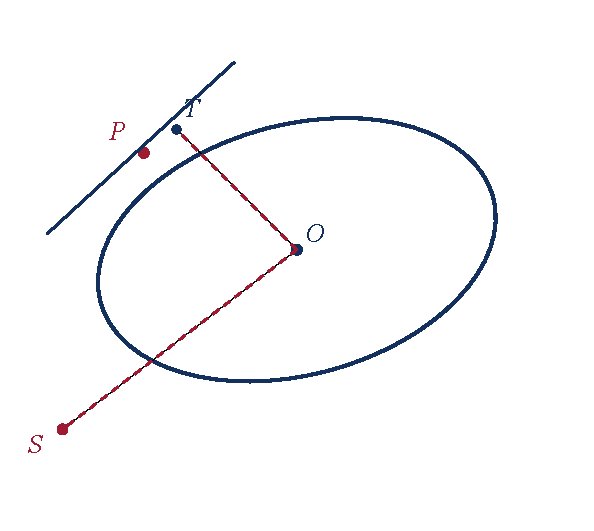
\includegraphics[width=0.5\textwidth]{figuras/pdf/cap06-fig1.pdf}
\caption{El elipsoide $\mathrm F=1$: el punto $\mathrm P$, el plano
tangente en $\mathrm P$, el pie de la perpendicular $\mathrm T$ desde el
centro $\mathrm O$, y el punto $\mathrm S$ sobre $\mathrm{OT}$ tal que
$\mathrm{OS}=1/\mathrm{OT}$.}
\label{fig:cap6-1}
\end{figure}

\section{Superficie de onda. Propagación rectilínea de la luz}

\subsection{Superficie de onda}

\noindent\textbf{180. Superficie de onda.} — Si suponemos el éter
primitivamente en reposo y que, en el origen de los tiempos, se perturban
las moléculas contenidas en una esfera de radio muy pequeño, las moléculas
en movimiento al cabo de la unidad de tiempo pertenecerán a una cierta
superficie que se llama \emph{superficie de onda}.

Esta superficie es una esfera en un medio isótropo. Extendiendo a los
cuerpos no isótropos el principio de Huygens, se puede hallar la ecuación
de la superficie de onda en esos medios cuando se conoce la velocidad de
propagación de una onda plana. Pero se pueden hacer a esta extensión del
principio de Huygens las objeciones que señalamos en el caso de los
isótropos, y para ser rigurosos, nos haría falta reemprender para los
cuerpos anisótropos la justificación a la que llegamos en el capítulo III.
Nos limitaremos a admitir la manera de razonar de Huygens sin buscar su
justificación.

Consideremos una onda plana $PP'$ (figura~\ref{fig:cap6-2}) que pasa por
un punto $O$ de un medio anisótropo. Al cabo de la unidad de tiempo, esta
onda coincidirá con el plano $QQ'$ paralelo a $PP'$, y situado a una
distancia de este último plano igual a la velocidad de propagación $V$ de
esta onda.

Por otra parte, la perturbación inicial del punto $O$ pondrá en
movimiento, al cabo del tiempo $1$, las moléculas del medio elástico que,
según la definición de la superficie de onda, están situadas en la
superficie de onda $S$ relativa al punto $O$. Ahora bien, según el
principio de Huygens, el movimiento del éter en todo punto de la onda
plana $QQ'$ es la resultante de los movimientos que envían aisladamente
cada uno de los puntos $O,O'$ de la onda $PP'$. Siendo $S,S',\dots$ las
ondas elementales de estos puntos, no puede haber movimiento más allá del
plano tangente común $Q_1Q_1'$ a estas ondas.\footnote{Corrección indicada
en la fe de erratas del propio volumen original, que pide rotular $Q_1Q_1'$
la recta superior de la figura, impresa también como $QQ'$.~(N.~del T.)} Además, lo hay ciertamente
en el punto $Q_1$ donde este plano toca a la superficie $S$; pues,
$Q_1$ siendo exterior a las demás superficies de onda $S',\dots$, el
movimiento enviado a $Q_1$ por el punto $O$ no puede ser destruido por el
movimiento enviado por los demás puntos del plano $PP'$. Y como el
movimiento no debe tener lugar más que en el plano $QQ'$, los dos planos
$QQ'$ y $Q_1Q_1'$ deben confundirse.

Cualquiera que sea la dirección del plano de la onda $PP'$ que pasa por el
punto $O$, la superficie de onda de este punto será siempre tangente a la
posición ocupada por la onda plana al cabo de la unidad de tiempo; por
consiguiente, es la envolvente de estas posiciones.

\begin{figure}[ht]
\centering
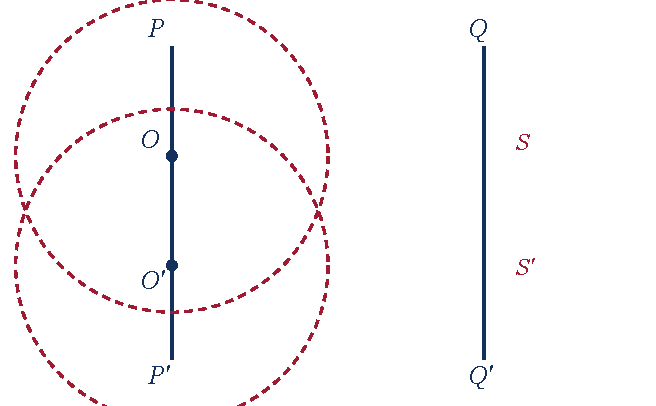
\includegraphics[width=0.75\textwidth]{figuras/pdf/cap06-fig2.pdf}
\caption{Dos posiciones sucesivas de una onda plana, $PP'$ y $QQ'$; las
ondas elementales $S,S'$ de los puntos $O,O'$ y su plano tangente común
$Q_1Q_1'$, que según el principio de Huygens debe confundirse con $QQ'$.}
\label{fig:cap6-2}
\end{figure}

\subsection{Dirección del rayo luminoso}

\noindent\textbf{181. Dirección del rayo luminoso.} — He aquí cómo se
puede, apoyándose en el principio de Huygens, determinar la dirección del
rayo luminoso. Sea $P$ (figura~\ref{fig:cap6-3}) la posición del plano de
la onda en un instante cualquiera, y $P'$ la nueva posición del plano de
la onda al cabo de la unidad de tiempo.

Supongamos ahora que el plano $P$ no esté perturbado en su totalidad, y
que la parte iluminada de este plano se reduzca a un elemento $AB$, con su
centro de gravedad en $O$, muy pequeño en términos absolutos, pero lo
bastante grande, sin embargo, para que puedan despreciarse los fenómenos
de difracción.

Se obtendrá la porción iluminada del plano $P'$ construyendo las
superficies de onda que tienen por centros los diversos puntos de $AB$, y
se buscarán los puntos de contacto de estas superficies con el plano $P'$.
Los puntos así obtenidos formarán un elemento plano $A'B'$ con su centro
de gravedad en $O'$. La recta $OO'$ es entonces el rayo luminoso buscado,
de donde la siguiente regla:

\begin{enunciado}{Regla de Huygens para el rayo luminoso}
Se obtendrá la dirección del rayo luminoso uniendo el punto $O$ al punto
de contacto de la superficie de onda, que tiene su centro en $O$, con un
plano tangente paralelo al plano de la onda.
\end{enunciado}

Vamos a aplicar esta regla sin preocuparnos por las objeciones que suscita
el principio de Huygens. Daremos, por lo demás, más adelante (§189) una
demostración rigurosa.

\begin{figure}[ht]
\centering
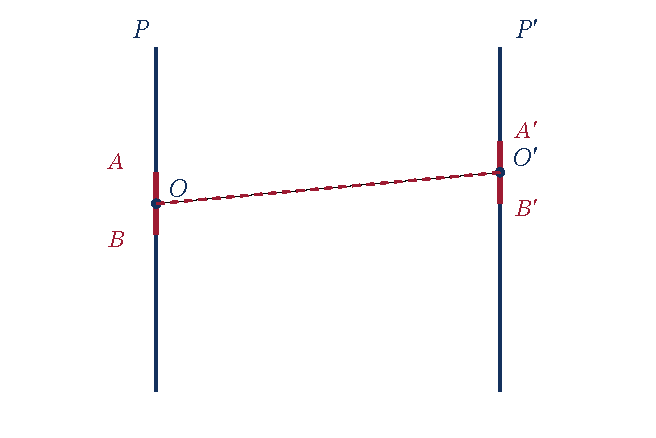
\includegraphics[width=0.6\textwidth]{figuras/pdf/cap06-fig3.pdf}
\caption{Construcción del rayo luminoso: el elemento iluminado $AB$ del
plano $P$, su imagen $A'B'$ en el plano $P'$, y el rayo $OO'$.}
\label{fig:cap6-3}
\end{figure}

\noindent\textbf{182.} Sean $\alpha,\beta,\gamma$ los cosenos directores
de la normal a una onda plana, $V$ la velocidad de propagación de esta
onda, y $x,y,z$ las coordenadas del punto donde la superficie de onda es
encontrada por el rayo luminoso que pasa por el origen. Perteneciendo
este punto al plano ocupado por la onda al cabo de la unidad de tiempo,
sus coordenadas satisfacen la ecuación
\begin{equation}
\alpha x+\beta y+\gamma z=\mathrm V;
\tag{1}
\end{equation}
como pertenece igualmente a la envolvente de este plano, se tiene también
\begin{equation}
x\,d\alpha+y\,d\beta+z\,d\gamma=d\mathrm V.
\tag{2}
\end{equation}
En cuanto a la velocidad de propagación $V$, sabemos que en todas las
teorías de la doble refracción que hemos expuesto, está dada por la
ecuación
\begin{equation}
\frac{\alpha^2}{\mathrm V^2-a}+\frac{\beta^2}{\mathrm V^2-b}+\frac{\gamma^2}{\mathrm V^2-c}=\mathrm F(\alpha,\beta,\gamma,\mathrm V)=0,
\tag{3}
\end{equation}
que, por diferenciación, da
\[
\frac{d\mathrm F}{d\alpha}d\alpha+\frac{d\mathrm F}{d\beta}d\beta+\frac{d\mathrm F}{d\gamma}d\gamma+\frac{d\mathrm F}{d\mathrm V}d\mathrm V=0.
\]
Reemplazando aquí $d\mathrm V$ por el primer miembro de la igualdad (2),
esta ecuación se convierte en
\begin{equation}
\Bigl(\frac{d\mathrm F}{d\alpha}+x\frac{d\mathrm F}{d\mathrm V}\Bigr)d\alpha
+\Bigl(\frac{d\mathrm F}{d\beta}+y\frac{d\mathrm F}{d\mathrm V}\Bigr)d\beta
+\Bigl(\frac{d\mathrm F}{d\gamma}+z\frac{d\mathrm F}{d\mathrm V}\Bigr)d\gamma=0.
\tag{4}
\end{equation}
Por lo demás, $\alpha,\beta,\gamma$ están ligados por la relación
$\alpha^2+\beta^2+\gamma^2=1$, que da por diferenciación
\begin{equation}
\alpha\,d\alpha+\beta\,d\beta+\gamma\,d\gamma=0.
\tag{5}
\end{equation}
Las dos relaciones (4) y (5), satisfechas a la vez para todos los valores
que se puedan dar a $d\alpha$ y $d\beta$, deben ser idénticas; tendremos,
pues, introduciendo una constante arbitraria $\mathrm K$,
\begin{equation}
\frac{d\mathrm F}{d\alpha}+x\frac{d\mathrm F}{d\mathrm V}=\mathrm K\alpha,\qquad
\frac{d\mathrm F}{d\beta}+y\frac{d\mathrm F}{d\mathrm V}=\mathrm K\beta,\qquad
\frac{d\mathrm F}{d\gamma}+z\frac{d\mathrm F}{d\mathrm V}=\mathrm K\gamma.
\tag{6}
\end{equation}

Busquemos los valores de $K$ y de las
derivadas parciales que entran en estas ecuaciones. Para ello recordemos
que la velocidad de propagación $V$ satisface las ecuaciones
\begin{equation}
\mathrm{AV}^2=a\mathrm A-\alpha\mathrm H,\qquad
\mathrm{BV}^2=b\mathrm B-\beta\mathrm H,\qquad
\mathrm{CV}^2=c\mathrm C-\gamma\mathrm H,
\tag{I}
\end{equation}
donde
\[
\mathrm H=\mathrm Aa\alpha+\mathrm Bb\beta+\mathrm Cc\gamma,
\]
y que, por eliminación de $H$, nos condujeron (§154) a la ecuación (3).
Tendremos
\[
\frac{d\mathrm F}{d\alpha}=\frac{2\alpha}{\mathrm V^2-a},
\]
y, reemplazando $\mathrm V^2-a$ por su valor tomado de la primera de las
ecuaciones del grupo (I),
\[
\frac{d\mathrm F}{d\alpha}=-\frac{2\mathrm A}{\mathrm H}.
\]
Hallaremos, de la misma manera, $d\mathrm F/d\beta=-2\mathrm B/\mathrm H$,
$d\mathrm F/d\gamma=-2\mathrm C/\mathrm H$.

Para la derivada respecto de $V$ tendremos
\[
\frac{d\mathrm F}{d\mathrm V}=-\sum\frac{2\alpha^2\mathrm V}{(\mathrm V^2-a)^2}
=-2\mathrm V\sum\frac{\alpha^2}{(\mathrm V^2-a)^2}
=-\frac{2\mathrm V}{\mathrm H^2}\sum\mathrm A^2.
\]
Ahora bien, hemos visto (§155) que si el punto $A,B,C$ está sobre el
elipsoide de elasticidad, se tiene
\[
\mathrm V=\frac{1}{\sqrt{\mathrm A^2+\mathrm B^2+\mathrm C^2}};
\]
resulta
\[
\frac{d\mathrm F}{d\mathrm V}=-\frac{2\mathrm V}{\mathrm H^2}\cdot\frac{1}{\mathrm V^2}=-\frac{2}{\mathrm{VH}^2}.
\]

Calculemos el coeficiente $K$. Para ello multipliquemos las ecuaciones (6)
por $\alpha,\beta,\gamma$ y sumemos; tendremos
\[
\mathrm K=\sum\alpha\frac{d\mathrm F}{d\alpha}+\frac{d\mathrm F}{d\mathrm V}\sum\alpha x;
\]
pero
\[
\sum\alpha\frac{d\mathrm F}{d\alpha}=-\sum\frac{2\mathrm A\alpha}{\mathrm H}=0,
\]
y, según la ecuación (1), $\sum\alpha x=\mathrm V$. Por consiguiente
\[
\mathrm K=\frac{d\mathrm F}{d\mathrm V}\,\mathrm V=-\frac{2}{\mathrm H^2}.
\]
Llevando estos valores de $K$ y de las derivadas parciales a las
ecuaciones (6), y multiplicando después por $-\mathrm H^2/2$,\footnote{El
original dice «multipliant par $-\frac{2}{\mathrm H^2}$»; es por
$-\frac{\mathrm H^2}{2}$ por lo que hay que multiplicar para obtener las
ecuaciones (II).~(N.~del T.)}
obtendremos
\begin{equation}
\mathrm{AH}+\frac{x}{\mathrm V}=\alpha,\qquad
\mathrm{BH}+\frac{y}{\mathrm V}=\beta,\qquad
\mathrm{CH}+\frac{z}{\mathrm V}=\gamma,
\tag{II}
\end{equation}
ecuaciones que nos darán las coordenadas $x,y,z$ del punto de
intersección de la superficie de onda por el rayo luminoso.

\subsection{Relaciones entre la dirección del rayo luminoso y las de las
vibraciones}

\noindent\textbf{183. Relaciones entre la dirección del rayo luminoso y
las de las vibraciones.} — Consideremos la vibración de Neumann, cuyos cosenos directores son
proporcionales a $A',B',C'$. Si multiplicamos las ecuaciones del grupo
(II) por $A',B',C'$ obtenemos, para la suma de estos productos,
\[
\mathrm H\sum\mathrm{AA}'+\frac1{\mathrm V}\sum\mathrm A'x=\sum\mathrm A'\alpha.
\]
Sabemos, por lo demás, que la vibración de Neumann está situada en el
plano de la onda y que es perpendicular a la de Fresnel; por consiguiente,
tendremos
\[
\mathrm A'\alpha+\mathrm B'\beta+\mathrm C'\gamma=0,\qquad
\mathrm{AA}'+\mathrm{BB}'+\mathrm{CC}'=0,
\]
y la relación precedente se reducirá a la siguiente
\[
\mathrm A'x+\mathrm B'y+\mathrm C'z=0,
\]
que expresa que \emph{la vibración de Neumann es perpendicular al rayo
luminoso}.

Tomemos ahora la vibración de M.~Sarrau, cuyos cosenos directores son
proporcionales a $\mathrm{A}a,\mathrm{B}b,\mathrm{C}c$. Multiplicando
respectivamente cada una de las ecuaciones (II) por estas cantidades y
sumando, tenemos
\[
\mathrm H\sum a\mathrm A^2+\frac1{\mathrm V}\sum a\mathrm Ax=\sum\mathrm Aa\alpha.
\]
El punto de coordenadas $A,B,C$ estando sobre el elipsoide de elasticidad,
$\sum a\mathrm A^2=1$; por otra parte, por hipótesis, $\mathrm
H=\sum\mathrm Aa\alpha$. Por consiguiente, la relación precedente se
reduce a la siguiente
\[
a\mathrm Ax+b\mathrm By+c\mathrm Cz=0,
\]
que expresa que \emph{la vibración de M.~Sarrau es perpendicular al rayo
luminoso}.

\subsection{Ecuación de la superficie de onda}

\noindent\textbf{184. Ecuación de la superficie de onda.} — La ecuación
de esta superficie se obtendrá eliminando $\alpha,\beta,\gamma,A,B,C$ y
$V$ entre las ecuaciones que forman los grupos (I) y (II) y la siguiente
\begin{equation}
\mathrm{A}ax+\mathrm{B}by+\mathrm{C}cz=0,
\tag{IV}
\end{equation}
que acabamos de deducir del grupo (II).

La primera de las ecuaciones (II) puede escribirse
\[
\frac{x\mathrm H}{\mathrm V}=\alpha\mathrm H-\mathrm{AH}^2,
\]
y la primera de las ecuaciones (I) nos da
\[
\alpha\mathrm H=\mathrm A(a-\mathrm V^2).
\]
Tendremos, pues,
\[
\frac{x\mathrm H}{\mathrm V}=\mathrm A(a-\mathrm V^2-\mathrm H^2).
\]
Busquemos el valor de $V^2+H^2$. Para ello saquemos de las ecuaciones
(II) los valores de $x,y,z$ y formemos los cuadrados de estas cantidades;
tendremos:
\[
x=\alpha\mathrm V-\mathrm{AHV},\qquad x^2=\alpha^2\mathrm V^2-2\mathrm A\alpha\mathrm{HV}^2+\mathrm A^2\mathrm H^2\mathrm V^2,
\]
\[
y=\beta\mathrm V-\mathrm{BHV},\qquad y^2=\beta^2\mathrm V^2-2\mathrm B\beta\mathrm{HV}^2+\mathrm B^2\mathrm H^2\mathrm V^2,
\]
\[
z=\gamma\mathrm V-\mathrm{CHV},\qquad z^2=\gamma^2\mathrm V^2-2\mathrm C\gamma\mathrm{HV}^2+\mathrm C^2\mathrm H^2\mathrm V^2,
\]
y por consiguiente
\[
x^2+y^2+z^2=r^2=\mathrm V^2-2\mathrm{HV}^2\sum\mathrm A\alpha+\mathrm H^2\mathrm V^2\sum\mathrm A^2.
\]
Ya hemos visto que $\sum\mathrm A\alpha=0$ y $\sum\mathrm A^2=1/\mathrm
V^2$; por consiguiente tendremos, para el cuadrado del radio vector de la
superficie de onda,
\[
r^2=\mathrm V^2+\mathrm H^2.
\]
Llevando este valor de $V^2+H^2$ a la expresión antes obtenida de
$xH/V$, obtendremos
\[
\frac{x\mathrm H}{\mathrm V}=\mathrm A(a-r^2),\qquad\text{o bien}\qquad
\frac{x}{r^2-a}=-\frac{\mathrm{AV}}{\mathrm H},
\]
y, por simetría,
\[
\frac{y}{r^2-b}=-\frac{\mathrm{BV}}{\mathrm H},\qquad
\frac{z}{r^2-c}=-\frac{\mathrm{CV}}{\mathrm H}.
\]
Tenemos así cantidades proporcionales a $A,B,C$ que, llevadas en lugar de
$A,B,C$ a la ecuación (IV), nos darán
\[
\frac{ax^2}{r^2-a}+\frac{by^2}{r^2-b}+\frac{cz^2}{r^2-c}=0;
\]
esta es la ecuación de la superficie de onda bajo su forma más simple.

Esta superficie parece ser de sexto grado; es fácil mostrar, desarrollando
la ecuación precedente, que es solamente de cuarto grado. Se tendrá,
quitando los denominadores,\footnote{El original imprime
$\sum ax^2(r^2-b^2)(r^2-c^2)=0$; los denominadores son $r^2-b$ y $r^2-c$,
como lo confirma el desarrollo que sigue.~(N.~del T.)}
\[
\sum ax^2(r^2-b)(r^2-c)=0,
\]
o bien
\[
r^4\sum ax^2-r^2\sum(b+c)ax^2+abc(x^2+y^2+z^2)=0.
\]
$r^2$ se encuentra, pues, en factor; suprimiendo este factor se obtiene
\[
\sum x^2\sum ax^2-\sum(ab+ac)x^2+abc=0,
\]
ecuación que no es más que de cuarto grado.

\subsection{Construcción geométrica de la superficie de onda}

\noindent\textbf{185. Construcción geométrica de la superficie de onda.}
— Consideremos una onda plana y tomemos como plano de la figura un plano
perpendicular al plano de onda y que pase por la vibración de Fresnel.
Esta vibración estará representada por la recta $OF$ (figura~\ref{fig:cap6-4}).
La vibración de Neumann, situada en el plano de la onda y perpendicular a
la de Fresnel, será normal al plano de la figura y se proyectará en el
punto $O$. El rayo luminoso y la vibración de M.~Sarrau, ambos
perpendiculares a la vibración de Neumann, estarán situados en el plano
del cuadro; sean $OS$ la vibración de M.~Sarrau, $OM$ el rayo luminoso,
rectas que son rectangulares entre sí. La posición del plano de la onda
al cabo de la unidad de tiempo está representada por su traza $PM$.

El plano tangente al elipsoide de elasticidad $ax^2+by^2+cz^2=1$ en el
punto $F$ de coordenadas $A,B,C$ tiene por ecuación
\[
a\mathrm Ax+b\mathrm By+c\mathrm Cz=1.
\]
Los cosenos directores de la normal a este plano son proporcionales a
$a\mathrm A,b\mathrm B,c\mathrm C$, es decir, a las componentes de la
vibración de M.~Sarrau. Este plano tangente será, pues, perpendicular al
plano de la figura, en la cual estará representado por la perpendicular
$FQ$ sobre $OS$. — Este resultado puede obtenerse de otra manera. La
recta $OF$ es un eje de la elipse de intersección $E$ del elipsoide de
elasticidad por el plano de la onda; por consiguiente, la tangente en $F$
a esta elipse es perpendicular a $OF$, y, estando además situada en el
plano de la onda, perpendicular al plano de la figura, es ella misma
perpendicular a este último plano. El plano tangente al elipsoide en $F$
que contiene esta tangente será también perpendicular al plano de la
figura.

Consideremos la esfera descrita desde el punto $O$ como centro con un
radio igual a la unidad. Si tomamos sobre la recta $OQ$ una longitud
$OS=1/OQ$, el punto $S$ es el polo del plano $FQ$ respecto a esta esfera.
Por consiguiente, el lugar del punto $S$ cuando el punto $F$ describe el
elipsoide de elasticidad será la polar recíproca del elipsoide de
elasticidad. Este elipsoide recíproco tiene, pues, por ecuación
\[
\frac{x^2}{a}+\frac{y^2}{b}+\frac{z^2}{c}=1.
\]
Tracemos el plano tangente en $S$ a este elipsoide; tiene por polo el
punto $F$; por consiguiente, es perpendicular al rayo $OF$, y corta el
plano de la figura según $ST$. Vamos a deducir que la recta $OS$ es un
eje de la elipse de intersección $E'$ del elipsoide recíproco $S$ por un
plano perpendicular al rayo luminoso. En efecto, la tangente en $S$ a esta
elipse está situada en el plano de sección y en el plano tangente al
elipsoide; estando estos dos planos perpendiculares al plano de la
figura, la tangente es también perpendicular a este último plano, y, por
consiguiente, al radio vector $OS$, que debe entonces ser un eje.

Mostremos ahora que se tiene $OM=OS$. Las rectas $OM$ y $OP$ siendo
respectivamente perpendiculares a $OS$ y $OF$, los ángulos $FOS$ y $POM$
son iguales. Tendremos, pues, puesto que $OP$, velocidad de propagación
normal de una onda plana, es igual al inverso del eje $OF$ de la elipse
$E$,
\[
OM=\frac{OP}{\cos\theta}=\frac{1}{OF\cos\theta}.
\]
Por otra parte, el triángulo $OFQ$ nos da
\[
OS=\frac{1}{OQ}=\frac{1}{OF\cos\theta}.
\]
Tenemos, pues, en efecto, $OM=OS$.

El punto $M$ siendo un punto de la superficie de onda, podremos construir
esta superficie de la manera siguiente: cortar el elipsoide recíproco $S$
por un plano cualquiera, y llevar sobre la normal $OM$ a este plano
longitudes iguales a los ejes de la elipse $E'$ de intersección.

\begin{figure}[ht]
\centering
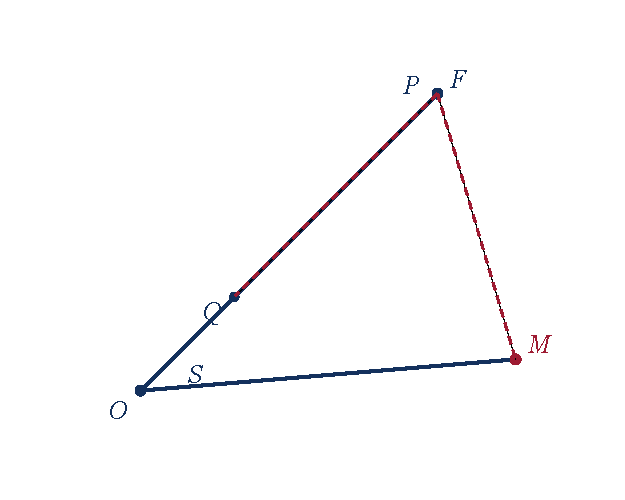
\includegraphics[width=0.85\textwidth]{figuras/pdf/cap06-fig4.pdf}
\caption{Construcción geométrica de la superficie de onda: la vibración
de Fresnel $OF$, el punto $Q$, la vibración de M.~Sarrau $OS$ y el rayo
luminoso $OM$.}
\label{fig:cap6-4}
\end{figure}

\subsection{Secciones de la superficie de onda por los planos de simetría}

\noindent\textbf{186. Secciones de la superficie de onda por los planos
de simetría.} — Tomemos como planos de la figura uno de los tres planos
de simetría óptica del medio. Siendo estos planos los planos principales
del elipsoide de elasticidad, serán igualmente los planos principales del
elipsoide recíproco $S$. Un plano perpendicular al plano de la figura y
que pase por el centro de este elipsoide contendrá, pues, uno de sus
ejes, el que es perpendicular al plano de la figura. Si $OS$
(figura~\ref{fig:cap6-5}) es el plano de sección considerado, se tendrán
los dos puntos correspondientes de la superficie de onda llevando sobre
la normal $OM$ a este plano la longitud $OM=OS$ y la longitud $OM'$ igual
al eje proyectado en $O$. Los dos puntos $M$ y $M'$ están situados en el
plano de la figura, y se obtendrá la intersección de la superficie de
onda por este plano haciendo girar el plano $OS$ alrededor de la normal
que pasa por $O$. Siendo constante uno de los ejes de las secciones así
obtenidas, el eje proyectado en $O$, la longitud $OM'$ será constante y
el punto $M'$ describirá un círculo. El punto $M$ describirá una elipse
que no es otra que la elipse $AB$ de intersección del elipsoide
recíproco por el plano de la figura, elipse cuyos ejes se han hecho girar
$90^{\circ}$.

La intersección de la superficie de onda por cada uno de los planos de
simetría se compone, pues, de un círculo y de una elipse. El conocimiento
de estas intersecciones permite darse bastante bien cuenta de la forma de
la superficie de onda. Si suponemos que se tenga $a>b>c$, la parte de la
superficie de onda comprendida en el triedro donde las tres coordenadas de
un punto son positivas tendrá la forma representada por la
figura~\ref{fig:cap6-6}.

En el caso particular de cristales de un eje, el elipsoide de elasticidad
es de revolución; el elipsoide recíproco, y por consiguiente la superficie
de onda, lo son igualmente. La intersección de esta superficie por dos de
los planos de simetría se compone de una elipse y de un círculo; la
intersección por el tercer plano de simetría está formada por dos
círculos. — La superficie de onda se compone entonces de una esfera y de
un elipsoide de revolución tangentes.

\begin{figure}[ht]
\centering
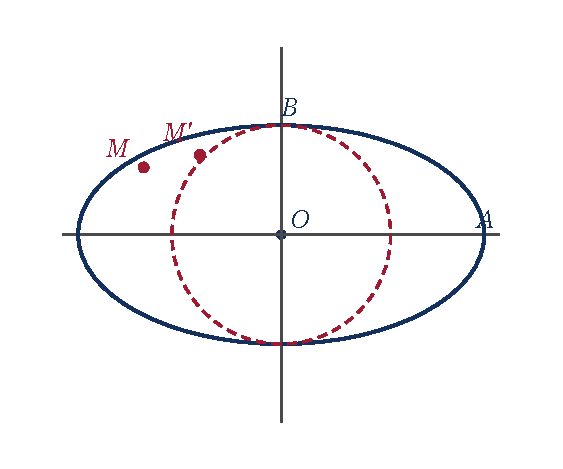
\includegraphics[width=0.75\textwidth]{figuras/pdf/cap06-fig5.pdf}
\caption{Sección de la superficie de onda por un plano de simetría: el
círculo y la elipse $AB$ del elipsoide recíproco.}
\label{fig:cap6-5}
\end{figure}

\begin{figure}[ht]
\centering
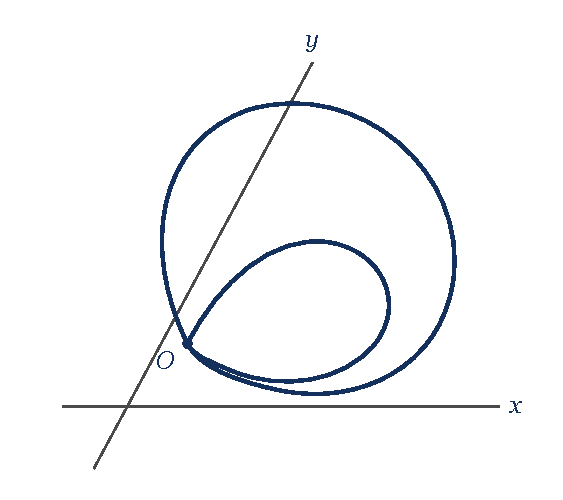
\includegraphics[width=0.6\textwidth]{figuras/pdf/cap06-fig6.pdf}
\caption{Forma de la superficie de onda en el triedro de coordenadas
positivas, para $a>b>c$: la curva compuesta que resulta de las dos hojas
(elipsoidal y esférica) de la superficie.}
\label{fig:cap6-6}
\end{figure}

\subsection{Ombligos y planos tangentes singulares de la superficie de
onda}

\noindent\textbf{187. Ombligos y planos tangentes singulares de la
superficie de onda.} — Consideremos un plano cíclico del elipsoide
recíproco. Todos los radios vectores de esta sección serán ejes iguales; por
consiguiente, a un plano cíclico no corresponde más que un solo punto $M$
de la superficie de onda. Pero, a cada dirección $OS$ de un eje
corresponde un plano tangente normal al plano que pasa por $OS$ y $OM$;
tendremos, pues, una infinidad de planos tangentes en $M$. Es un punto
cónico. Como a cada sección cíclica corresponden dos puntos cónicos,
tendremos cuatro puntos cónicos reales y ocho puntos cónicos imaginarios.
A estos puntos se les llama también los \emph{ombligos} de la superficie
de onda.

El cono formado por los planos tangentes a la superficie de onda en un
punto cónico es de segundo grado. En efecto, no puede ser de tercer
grado, pues la recta que pasa por dos de estos puntos encontraría a la
superficie en seis puntos, lo que no puede ocurrir puesto que esta
superficie es de cuarto grado.

La consideración de los planos cíclicos del elipsoide de elasticidad
conduce a una nueva propiedad interesante de la superficie de onda.

Si suponemos que el plano de la onda sea un plano cíclico, todo radio del
círculo de intersección será una dirección de la vibración de Fresnel. A
cada una de estas direcciones corresponde un plano tangente $PM$ a la
superficie de onda; pero, como $OP=1/OF$ y $OF$ es constante, estos
diversos planos tangentes se confunden. Sus puntos de contacto con la
superficie de onda no se confunden, sin embargo, pues a cada dirección de
$OF$ corresponde una dirección particular de $OS$ y, por consiguiente, de
$OM$. Por consiguiente, el plano $PM$ correspondiente a una sección
circular del elipsoide toca la superficie de onda en una infinidad de
puntos distintos. Estos puntos forman una curva que debe ser de segundo
grado, pues, en general, la sección de una superficie por un plano
tangente singular, componiéndose de dos curvas confundidas, cada una de
estas curvas es de un grado igual a la mitad del grado de la superficie.
Además, esta curva de segundo grado es un círculo. En efecto, las
direcciones asintóticas de la superficie están dadas por los términos del
más alto grado $\sum x^2\sum ax^2$; dos de estas direcciones son las de
un círculo, y, como para los planos tangentes singulares las direcciones
asintóticas deben confundirse dos a dos, puesto que las curvas de
intersección se confunden, las cuatro direcciones asintóticas son las de
círculos. La curva de intersección de la superficie por un plano tangente
singular se compone, pues, de dos círculos confundidos. Habrá cuatro de
estos planos tangentes singulares, que serán reales, un elipsoide teniendo
dos direcciones de secciones cíclicas a cada una de las cuales
corresponden dos planos tangentes singulares.

Muchas otras propiedades de la superficie de onda han sido estudiadas por
diversos matemáticos. En particular, citaremos los procedimientos
elegantes indicados por M.~Mannheim para hallar los radios de curvatura y
trazar las líneas de curvatura de la superficie de onda. Pero no
insistiremos en estas propiedades, que no tienen ningún interés desde el
punto de vista de la óptica. Solo la consideración de los ombligos y de
los planos tangentes singulares tiene una gran importancia. Se sabe, en
efecto, que condujo a Hamilton al descubrimiento de la \emph{refracción
cónica interior} y de la \emph{refracción cónica exterior} que Lloyd pudo
poner en evidencia mediante experiencias delicadas.

\begin{notahistorica}
La refracción cónica, predicha teóricamente por William Rowan Hamilton en
1832 a partir de los puntos cónicos y de los planos tangentes singulares
de la superficie de onda de Fresnel, fue confirmada experimentalmente muy
poco después por Humphrey Lloyd, quien la observó en el aragonito y
publicó sus resultados en 1833. Es uno
de los ejemplos más citados de un fenómeno físico descubierto primero por
el análisis matemático y solo después observado en el laboratorio.
\end{notahistorica}

\section{Propagación rectilínea de la luz}

\subsection{Propagación rectilínea de la luz en un medio isótropo}

\noindent\textbf{188. Propagación rectilínea de la luz en un medio
isótropo.} — Hemos determinado más arriba (§181) la dirección del rayo
luminoso en un medio cristalizado apoyándonos en el principio de Huygens;
pero este principio, cualesquiera que sean la utilidad y la importancia de
su papel en óptica, se presta a un gran número de objeciones de las que
hemos tratado de dar una idea en la primera parte del curso.

Por eso no será inútil explicar aquí cómo se puede determinar la
dirección del rayo luminoso en un medio isótropo o anisótropo
independizándose del principio de Huygens y de las dificultades sin
cuento que suscita. Comenzaremos por el caso más simple, que es el de los
medios isótropos, y escribiremos las ecuaciones del movimiento
transversal bajo la forma habitual,
\[
\rho\,\frac{d^2\xi}{dt^2}=\Delta\xi,\qquad
\rho\,\frac{d^2\eta}{dt^2}=\Delta\eta,\qquad
\rho\,\frac{d^2\zeta}{dt^2}=\Delta\zeta,
\]
con $\Theta=0$.

Busquemos satisfacer estas ecuaciones haciendo:
\begin{equation}
\xi=Ae^{\mathrm P},\qquad \eta=Be^{\mathrm P},\qquad \zeta=Ce^{\mathrm P},
\tag{1}
\end{equation}
donde
\[
\mathrm P=\frac{2i\pi}{\lambda}(z-\mathrm Vt).
\]
Si consideráramos $A,B,C$ como constantes, caeríamos de nuevo en la
teoría ordinaria de la propagación de una onda plana indefinida. Pero
entonces la cuestión de la dirección del rayo luminoso no se plantearía,
puesto que todo el espacio quedaría igualmente iluminado. Debemos, pues,
suponer que solo una porción del éter es agitada por ondulaciones y, por
consiguiente, que $A,B,C$ son funciones de $x,y,z$ y $t$.

Tomaremos una unidad de longitud comparable a nuestras unidades
habituales, de tal manera que $\lambda$ será una longitud muy pequeña y
$2i\pi/\lambda$ una cantidad infinitamente grande; (si en la exposición
de la teoría de M.~Sarrau consideramos esta cantidad como muy pequeña, es
porque habíamos tomado una unidad de longitud comparable a la distancia
que separa dos moléculas materiales). Por el contrario, supondremos que
las funciones $A,B,C$ y sus derivadas de los diversos órdenes son
finitas.

Las consideraciones que siguen no se aplican, pues, al menos sin
modificación, al caso en que las funciones $A,B,C$ son discontinuas y en
que, por consiguiente, sus derivadas no son finitas; en ese caso, en
efecto, se producen fenómenos de difracción y hay desviación del rayo
luminoso.

Sustituyamos los valores (1) en la primera de las ecuaciones del
movimiento; vendrá, dividiendo por $-e^{\mathrm P}4\pi^2/\lambda^2$,
\[
\rho\Bigl(\mathrm V^2\mathrm A-\frac{\lambda}{i\pi}\mathrm V\frac{dA}{dt}-\frac{\lambda^2}{4\pi^2}\frac{d^2A}{dt^2}\Bigr)
=A+\frac{\lambda}{i\pi}\frac{dA}{dz}-\frac{\lambda^2}{4\pi^2}\Delta A.
\]
Despreciaremos los términos en $\lambda^2$; si observamos que $\rho
V^2=1$, veremos que los términos independientes de $\lambda$
desaparecen; los dos miembros contendrán entonces el factor $\lambda/i\pi$.
Si hacemos desaparecer este factor, quedará simplemente
\begin{equation}
\frac{dA}{dt}+\mathrm V\frac{dA}{dz}=0.
\tag{2}
\end{equation}
Se hallaría del mismo modo
\[
\frac{dB}{dt}+\mathrm V\frac{dB}{dz}=0,\qquad
\frac{dC}{dt}+\mathrm V\frac{dC}{dz}=0.
\]
Si sustituimos los valores (1) en la ecuación $\Theta=0$ y la dividimos
por $e^{\mathrm P}$, vendrá
\[
\frac{2i\pi}{\lambda}C+\frac{dA}{dx}+\frac{dB}{dy}+\frac{dC}{dz}=0.
\]
Esta ecuación nos muestra que $C$ es un infinitamente pequeño del mismo
orden que $\lambda$. En cuanto a la ecuación (2), tiene por integral
general:
\[
A=\text{función arbitraria de }x,y\text{ y }z-\mathrm Vt.
\]
Así, el valor de $A$ en el tiempo $t$ y en el punto cuyas coordenadas son
$x,y$ y $z+\mathrm Vt$, será el mismo que en el tiempo $0$ y en el punto
$x,y,z$. Si en el origen de los tiempos no hay luz sensible más que en el
interior de una pequeña esfera que tenga por centro el punto $x,y,z$; en
la época $t$, no habrá luz sensible más que en el interior de una
pequeña esfera del mismo radio que tenga por centro el punto $x,y$ y
$z+\mathrm Vt$. En otros términos, la luz se habrá propagado en la
dirección del eje de las $z$, es decir, perpendicularmente al plano de la
onda.

Así, \emph{en un medio isótropo el rayo luminoso es normal al plano de la
onda.}

\subsection{Propagación rectilínea de la luz en un medio anisótropo}

\noindent\textbf{189. Propagación rectilínea de la luz en un medio
anisótropo.} — Pasemos al caso de un medio cristalizado, y tomemos por
ejemplo las ecuaciones de M.~Sarrau:
\begin{equation}
\frac1a\frac{d^2\xi}{dt^2}=\Delta\xi-\frac{d\Theta}{dx},\qquad
\frac1b\frac{d^2\eta}{dt^2}=\Delta\eta-\frac{d\Theta}{dy},\qquad
\frac1c\frac{d^2\zeta}{dt^2}=\Delta\zeta-\frac{d\Theta}{dz}.
\tag{1}
\end{equation}
Busquemos satisfacerlas poniendo
\[
\xi=\mathrm Le^{\mathrm P},\qquad \eta=\mathrm Me^{\mathrm P},\qquad
\zeta=\mathrm Ne^{\mathrm P},\qquad
\mathrm P=\frac{2i\pi}{\lambda}(\alpha x+\beta y+\gamma z-\mathrm Vt),
\]
siendo $L,M,N$ funciones de $x,y,z$ y $t$.

Si $L,M$ y $N$ debieran ser constantes $L_0,M_0,N_0$, estas constantes y
$V$ deberían satisfacer las ecuaciones\footnote{El original numera
también (1) este sistema, repitiendo el número de las ecuaciones del
movimiento que preceden; conservamos su numeración.~(N.~del T.)}
\begin{equation}
\frac{\mathrm V^2\mathrm L_0}{a}=\mathrm L_0-\alpha\mathrm H,\qquad
\frac{\mathrm V^2\mathrm M_0}{b}=\mathrm M_0-\beta\mathrm H,\qquad
\frac{\mathrm V^2\mathrm N_0}{c}=\mathrm N_0-\gamma\mathrm H,
\tag{1}
\end{equation}
\[
\mathrm H=\alpha\mathrm L_0+\beta\mathrm M_0+\gamma\mathrm N_0.
\]
Pongamos entonces:
\[
\mathrm L=\mathrm L_0f+g,\qquad \mathrm M=\mathrm M_0f+h,\qquad \mathrm N=\mathrm N_0f,
\]
y busquemos determinar las tres funciones $f,g$ y $h$.

Para obtener estas tres funciones, sustituyamos en las ecuaciones del
movimiento, en lugar de $\xi,\eta,\zeta$, sus valores, es decir,
\[
\xi=(\mathrm L_0f+g)e^{\mathrm P},\qquad \eta=(\mathrm M_0f+h)e^{\mathrm P},\qquad \zeta=\mathrm N_0fe^{\mathrm P}.
\]
Obtendremos así tres ecuaciones diferenciales entre $f,g$ y $h$. Según su
modo de formación, estas ecuaciones serán:

1.\textsuperscript{o} Lineales y homogéneas respecto a $f,g$ y $h$ y a sus
derivadas parciales de los dos primeros órdenes;

2.\textsuperscript{o} De coeficientes constantes, una vez suprimido el
factor común $e^{\mathrm P}$.

Eliminemos ahora $g$ y $h$ entre estas tres ecuaciones; quedará una
ecuación diferencial única que definirá a $f$. Esta ecuación será también
lineal, homogénea y de coeficientes constantes; pero será de orden
superior al segundo.

No contendrá a $f$, pues las ecuaciones del movimiento deben satisfacerse
cuando se hace
\[
f=1,\qquad g=h=0.
\]
No cambiará cuando se multipliquen a la vez $\lambda,x,y,z$ y $t$ por un
mismo factor, lo que equivale a cambiar simultáneamente y en una misma
razón la unidad de longitud y la del tiempo.

Sea
\[
\mathrm A\lambda^p\mathrm D^mf
\]
un término cualquiera del primer miembro de nuestra ecuación; $A$ es una
constante independiente de $\lambda$, y $D^mf$ una de las derivadas
parciales de orden $m$ de $f$. Cuando se cambien $\lambda,x,y,z$ y $t$ en
$k\lambda,kx,ky,kz$ y $kt$, este término quedará multiplicado por
$k^{p-m}$. Para que la ecuación no cambie, es preciso que $m-p$ tenga el
mismo valor para todos los términos de la ecuación. Multiplicaremos
nuestra ecuación por una potencia de $\lambda$ tal que $m-p$ sea igual a
$1$.

Entonces, los coeficientes de las derivadas de primer orden no
contendrán a $\lambda$; los de las derivadas de segundo orden contendrán
el factor $\lambda$; los de las derivadas de tercer orden contendrán el
factor $\lambda^2$; y así sucesivamente. Pero, siendo $\lambda$ muy
pequeño, podemos despreciar los términos que contienen este factor; no
nos quedarán entonces más que las derivadas de primer orden, y la
ecuación en $f$ se escribirá
\[
\mu\frac{df}{dx}+\mu'\frac{df}{dy}+\mu''\frac{df}{dz}+\frac{df}{dt}=0,
\]
siendo $\mu,\mu',\mu''$ constantes.

La integral general de esta ecuación será:
\[
f=\text{función arbitraria de }x-\mu t,\ y-\mu't\text{ y }z-\mu''t,
\]
lo que quiere decir que los cosenos directores del rayo luminoso son
proporcionales a $\mu,\mu'$ y $\mu''$, y que la velocidad de propagación,
estimada no normalmente al plano de la onda, sino en la dirección del
rayo, es $\sqrt{\mu^2+\mu'^2+\mu''^2}$.

Se podrían determinar $\mu,\mu'$ y $\mu''$ efectuando todos los cálculos
que acabamos de indicar; pero esto es inútil. En efecto, las ecuaciones
del movimiento deberán quedar satisfechas si se hace $f=e^{x-\mu t}$, de
donde $g$ y $h$ constante muy pequeña $\times\,e^{x-\mu t}$, y
\[
\mathrm L=\mathrm L_0e^{x-\mu t},\qquad \mathrm M=\mathrm M_0'e^{x-\mu t},\qquad \mathrm N=\mathrm N_0'e^{x-\mu t};
\]
$L_0,M_0'$ y $N_0'$ siendo constantes muy poco diferentes de $L_0,M_0$ y
$N_0$. Tendremos entonces
\[
\xi=\mathrm L_0e^{\mathrm P'},\qquad \eta=\mathrm M_0'e^{\mathrm P'},\qquad \zeta=\mathrm N_0'e^{\mathrm P'};
\]
\[
\mathrm P'=\frac{2i\pi}{\lambda}\Bigl[\Bigl(\alpha+\frac{\lambda}{2i\pi}\Bigr)x+\beta y+\gamma z-\Bigl(\mathrm V+\frac{\lambda\mu}{2i\pi}\Bigr)t\Bigr].
\]
Ahora bien, hemos visto que si $\xi,\eta,\zeta$ son iguales a constantes
multiplicadas por $e^{\mathrm P}$ y que se pone
\[
\mathrm P=\frac{2i\pi}{\lambda}(\alpha x+\beta y+\gamma z-\mathrm Vt)
\]
con $\lambda$ elegido de tal manera que $\alpha^2+\beta^2+\gamma^2=1$,
deberá tenerse
\[
\frac{\alpha^2}{\mathrm V^2-a}+\frac{\beta^2}{\mathrm V^2-b}+\frac{\gamma^2}{\mathrm V^2-c}=0.
\]
Designaremos, como ya lo hemos hecho más arriba, el primer miembro de
esta ecuación por
\[
\mathrm F(\alpha,\beta,\gamma,\mathrm V).
\]
Como $\alpha^2+\beta^2+\gamma^2=1$, tendremos también
\begin{equation}
\mathrm F\Bigl(\alpha,\beta,\gamma,\frac{\mathrm V}{\sqrt{\alpha^2+\beta^2+\gamma^2}}\Bigr)=0.
\tag{3}
\end{equation}
La relación (3), siendo homogénea en $\alpha,\beta,\gamma$ y $V$,
subsistirá aún cuando se hayan multiplicado a la vez $\alpha,\beta,\gamma$
y $V$ por un mismo factor. Es, pues, aún verdadera, incluso cuando ya no
se suponga que la suma $\alpha^2+\beta^2+\gamma^2$ sea igual a $1$.

Así, la relación (3) deberá quedar satisfecha cuando en ella se reemplacen
$\alpha,\beta,\gamma$ y $V$ por los coeficientes de $x,y,z$ y $-t$ en
$P'$, es decir, por
\[
\alpha+\frac{\lambda}{2i\pi},\qquad \beta,\qquad \gamma\qquad\text{y}\qquad
\mathrm V+\frac{\lambda\mu}{2i\pi}.
\]
Tendremos, pues,
\begin{equation}
\mathrm F\Bigl(\alpha+\frac{\lambda}{2i\pi},\beta,\gamma,
\frac{\mathrm V+\dfrac{\lambda\mu}{2i\pi}}{\sqrt{\bigl(\alpha+\dfrac{\lambda}{2i\pi}\bigr)^2+\beta^2+\gamma^2}}\Bigr)=0.
\tag{4}
\end{equation}
Esto es cierto con el grado de aproximación adoptado más arriba, es
decir, suponiendo que $\lambda$ es muy pequeño; se tiene entonces,
despreciando $\lambda^2$,\footnote{El original imprime
$\bigl(1+\frac{\alpha\lambda}{i\pi}\bigr)^{-\frac12}=1+\frac{\alpha\lambda}{2i\pi}$;
el signo correcto es $-$, que es el que se emplea en la igualdad
siguiente.~(N.~del T.)}
\[
\Bigl[\Bigl(\alpha+\frac{\lambda}{2i\pi}\Bigr)^2+\beta^2+\gamma^2\Bigr]^{-\frac12}
=\Bigl[(\alpha^2+\beta^2+\gamma^2)+\frac{\alpha\lambda}{i\pi}\Bigr]^{-\frac12}
=\Bigl(1+\frac{\alpha\lambda}{i\pi}\Bigr)^{-\frac12}=1-\frac{\alpha\lambda}{2i\pi},
\]
y
\[
\frac{\mathrm V+\dfrac{\lambda\mu}{2i\pi}}{\sqrt{\bigl(\alpha+\dfrac{\lambda}{2i\pi}\bigr)^2+\beta^2+\gamma^2}}
=\mathrm V+\frac{\lambda\mu}{2i\pi}-\frac{\alpha\mathrm V\lambda}{2i\pi},
\]
\begin{multline*}
\mathrm F\Bigl(\alpha+\frac{\lambda}{2i\pi},\beta,\gamma,
\frac{\mathrm V+\dfrac{\lambda\mu}{2i\pi}}{\sqrt{\bigl(\alpha+\dfrac{\lambda}{2i\pi}\bigr)^2+\beta^2+\gamma^2}}\Bigr)\\
=\mathrm F(\alpha,\beta,\gamma,\mathrm V)+\frac{\lambda}{2i\pi}\Bigl[\frac{d\mathrm F}{d\alpha}+\frac{d\mathrm F}{d\mathrm V}(\mu-\alpha\mathrm V)\Bigr].
\end{multline*}
Quedará, pues, teniendo en cuenta las relaciones (3) y (4):
\[
\frac{d\mathrm F}{d\alpha}+\mu\frac{d\mathrm F}{d\mathrm V}=\alpha\mathrm V\frac{d\mathrm F}{d\mathrm V},\qquad
\frac{d\mathrm F}{d\beta}+\mu'\frac{d\mathrm F}{d\mathrm V}=\beta\mathrm V\frac{d\mathrm F}{d\mathrm V},\qquad
\frac{d\mathrm F}{d\gamma}+\mu''\frac{d\mathrm F}{d\mathrm V}=\gamma\mathrm V\frac{d\mathrm F}{d\mathrm V}.
\]
Si se comparan estas ecuaciones con las ecuaciones (6) del §182, se verá
que el punto cuyas coordenadas son $\mu,\mu'$ y $\mu''$ no es otro que el
punto que hemos llamado $O'$ en ese párrafo (véase figura~\ref{fig:cap6-3})
y cuyas coordenadas estaban designadas por $x,y$ y $z$.

Como los cosenos directores del rayo luminoso son, según lo que acabamos
de ver, proporcionales a $\mu,\mu'$ y $\mu''$, la recta $OO'$ de la
figura~\ref{fig:cap6-3} es, en efecto, paralela al rayo luminoso; lo cual
está de acuerdo con el resultado al que nos había conducido la aplicación
del principio de Huygens.

\section{Doble refracción en los cristales hemiedros}

\subsection{Ecuaciones del movimiento}

\noindent\textbf{190. Ecuaciones del movimiento.} — Las teorías de la
doble refracción expuestas precedentemente no se aplican más que a los
medios holoedros. Para explicar los fenómenos que presentan los medios
birrefringentes hemiedros, debemos, como lo hicimos en la teoría de la
polarización rotatoria, rechazar la hipótesis del §14, en la que
admitíamos que en las expresiones de $\mathrm{D}\xi,\mathrm{D}\eta,\mathrm{D}\zeta$ los términos que
contienen los cuadrados de $\mathrm{D}x,\mathrm{D}y,\mathrm{D}z$ eran despreciables. Hemos visto que
si no se acepta esta hipótesis, la función $\mathrm{W}_2$ es una función homogénea
y de segundo grado de las derivadas parciales de los diversos órdenes de
$\xi,\eta,\zeta$, y que las ecuaciones del movimiento son
\[
\rho\,\frac{d^2\xi}{dt^2}=\mathrm P,\qquad
\rho\,\frac{d^2\eta}{dt^2}=\mathrm Q,\qquad
\rho\,\frac{d^2\zeta}{dt^2}=\mathrm R,
\]
siendo $P,Q,R$ polinomios lineales respecto a las derivadas de los
diversos órdenes de $\xi,\eta,\zeta$, polinomios cuyo modo de formación
hemos indicado (§124).

Si no se tiene en cuenta la dispersión, es inútil introducir las
derivadas parciales de cuarto orden. Pongamos, pues,
\[
\mathrm P=\mathrm X+\mathrm F,\qquad \mathrm Q=\mathrm Y+\mathrm G,\qquad \mathrm R=\mathrm Z+\mathrm H,
\]
siendo $X,Y,Z$ funciones lineales de las derivadas segundas de
$\xi,\eta,\zeta$, y $F,G,H$ funciones lineales de las derivadas de tercer
orden. Tomando unidades tales que $\rho$ sea igual a $1$, las ecuaciones
del movimiento son entonces
\[
\frac{d^2\xi}{dt^2}=\mathrm X+\mathrm F,\qquad
\frac{d^2\eta}{dt^2}=\mathrm Y+\mathrm G,\qquad
\frac{d^2\zeta}{dt^2}=\mathrm Z+\mathrm H.
\]
En el caso de los medios holoedros, estas ecuaciones deben necesariamente
reducirse a las que hemos tomado al comienzo de este capítulo y que nos
han conducido a la explicación de los fenómenos de doble refracción que
presentan esos medios. Mostremos que, en efecto, las cantidades $F,G,H$
desaparecen entonces de las ecuaciones precedentes.

Los medios holoedros, poseyendo tres planos de simetría óptica y, por
consiguiente, un centro de simetría, las ecuaciones que dan el movimiento
de una de sus moléculas no deben cambiar cuando se cambian los signos de
$x,y,z,\xi,\eta,\zeta$. Ahora bien, esta condición no quedaría satisfecha
si estas ecuaciones contuvieran una derivada de tercer orden,
$d^3\xi/dx^2dy$ por ejemplo, pues esta derivada conservaría su signo
mientras que las derivadas $d^2\xi/dt^2,\dots$, que forman los primeros
miembros, cambiarían de signo. Por lo demás ya hemos dicho (§124) que, de
manera general, las ecuaciones del movimiento en un medio que posee un
centro de simetría no podían contener más que derivadas de orden par.

\noindent\textbf{191.} Los coeficientes de los diferentes términos de los
polinomios $F,G,H$ no son independientes; vamos a mostrar que si el
polinomio $F$ contiene $\alpha\,d^3\eta/dx^2dy$, el polinomio $G$ contiene
$-\alpha\,d^3\xi/dx^2dy$.

Según el modo de formación del polinomio $P$, el término
$\alpha\,d^3\eta/dx^2dy$ de este polinomio debe provenir del término
$\alpha\,d\eta/dx\cdot d^2\xi/dxdy$ o $\alpha\eta_x'\xi_{xy}''$ de la
función $\mathrm{W}_2$. En efecto, si aplicamos este modo de formación deberemos
primero tomar la derivada de este término respecto a $\xi_{xy}''$, lo que
da $\alpha\eta_x'$, y luego tomar la derivada segunda de este resultado
respecto a $x$ y a $y$, lo que da $\alpha\,d^3\eta/dx^2dy$.

Si ahora buscamos los términos de $G$ que están dados por el término
$\alpha\eta_x'\xi_{xy}''$ de la función $\mathrm{W}_2$, uno de estos términos se
obtendrá derivando primero respecto a $\eta_x'$, luego derivando el
resultado respecto a $x$ y cambiando el signo. Efectuando estas
operaciones se encuentra, como lo habíamos anunciado, $-\alpha\,d^3\xi/dx^2dy$.

\subsection{Propagación de una onda plana}

\noindent\textbf{192. Propagación de una onda plana.} — Estudiemos,
tomando como punto de partida los trabajos de Neumann y Mac-Cullagh, la
propagación de una onda plana en un medio hemiedro.

Siendo cualesquiera los ejes a los que se refieren las ecuaciones del
movimiento, podemos considerar la onda plana como paralela al plano $xy$.
Entonces $\xi,\eta,\zeta$ no dependen más que de $z$ y de $t$, y las
derivadas de los desplazamientos respecto a $x$ y a $y$ desaparecen de
las ecuaciones del movimiento. Si los polinomios $F,G,H$ fueran nulos, las
vibraciones serían transversales; la condición $\Theta=0$ daría
$d\zeta/dz=0$ y las derivadas de $\zeta$ respecto a $z$ desaparecerían
también de las ecuaciones del movimiento. En general, cuando $F,G$ y $H$
son distintos de cero, ya no sucede así, pero siendo las vibraciones aún
casi transversales se pueden despreciar estas derivadas.

En estas condiciones las ecuaciones del movimiento en el plano de la onda
son
\[
\frac{d^2\xi}{dt^2}=a\frac{d^2\xi}{dz^2}+b\frac{d^2\eta}{dz^2}+\alpha\frac{d^3\xi}{dz^3}+\beta\frac{d^3\eta}{dz^3},
\]
\[
\frac{d^2\eta}{dt^2}=b\frac{d^2\xi}{dz^2}+c\frac{d^2\eta}{dz^2}-\beta\frac{d^3\xi}{dz^3}+\gamma\frac{d^3\eta}{dz^3};
\]
ecuaciones en las que los coeficientes satisfacen las relaciones
impuestas por el modo de formación de los segundos miembros.

Se simplifican cuando se toman como ejes de las
$x$ y de las $y$ las direcciones rectangulares de las dos vibraciones de
Neumann. Deben entonces quedar satisfechas para los valores de $\xi$ y
$\eta$ correspondientes a estas vibraciones cuando en ellos se desprecian
las derivadas de tercer orden. Ahora bien, si hacemos
$\xi=Ae^{\frac{2i\pi}{\lambda}(z-\mathrm Vt)},\eta=0$, coordenadas del
extremo de la vibración paralela al eje de las $x$, la segunda ecuación da
$b=0$. Por consiguiente, con esta elección de ejes de coordenadas, las
ecuaciones precedentes se reducen a
\[
\frac{d^2\xi}{dt^2}=a\frac{d^2\xi}{dz^2}+\alpha\frac{d^3\xi}{dz^3}+\beta\frac{d^3\eta}{dz^3},
\]
\[
\frac{d^2\eta}{dt^2}=c\frac{d^2\eta}{dz^2}-\beta\frac{d^3\xi}{dz^3}+\gamma\frac{d^3\eta}{dz^3}.
\]

\noindent\textbf{193.} Haciendo hipótesis
particulares sobre los coeficientes de los términos de $\mathrm{W}_2$ que
contienen derivadas segundas, y que, por consiguiente, dan los términos
$F,G,H$ de las ecuaciones del movimiento, Mac-Cullagh llegó a ecuaciones
en las que $\alpha=\gamma=0$. Vamos a mostrar que, sin hacer ninguna
hipótesis sobre la función $\mathrm{W}_2$, se tiene siempre $\alpha=\gamma=0$.

Según el modo de formación de los segundos miembros de las ecuaciones del
movimiento, el término de $\mathrm{W}_2$ que podría dar
$\alpha\,d^3\xi/dz^3$ en $F$ debería ser de la forma
$\alpha\,d\xi/dz\cdot d^2\xi/dz^2$ o $\alpha\xi_z'\xi_{zz}''$. Busquemos
los dos términos que este dará en $F$. Tendremos:
\[
\mathrm F=-\frac{d}{dz}\frac{d\alpha\xi_z'\xi_{zz}''}{d\xi_z'}
+\frac{d^2}{dz^2}\frac{d\alpha\xi_z'\xi_{zz}''}{d\xi_{zz}''}+\dots,
\]
\[
\mathrm F=-\frac{d}{dz}\alpha\xi_{zz}''+\frac{d^2}{dz^2}\alpha\xi_z'+\dots,
\]
o bien
\[
\mathrm F=-\alpha\frac{d^3\xi}{dz^3}+\alpha\frac{d^3\xi}{dz^3}+\dots.
\]
Por consiguiente, el único término de $\mathrm{W}_2$ capaz de dar un término en
$d^3\xi/dz^3$ en la primera ecuación da dos que se destruyen. Se vería de
la misma manera que $d^3\eta/dz^3$ no debe entrar en la segunda ecuación.
Tenemos, pues, para estas ecuaciones
\begin{equation}
\frac{d^2\xi}{dt^2}=a\frac{d^2\xi}{dz^2}+\beta\frac{d^3\eta}{dz^3},\qquad
\frac{d^2\eta}{dt^2}=c\frac{d^2\eta}{dz^2}-\beta\frac{d^3\xi}{dz^3}.
\tag{1}
\end{equation}

\subsection{Velocidades de propagación}

\noindent\textbf{194. Velocidades de propagación.} — Busquemos
satisfacer estas ecuaciones poniendo
\[
\xi=\mathrm Ae^{\frac{2i\pi}{\lambda}(z-\mathrm Vt)},\qquad
\eta=\mathrm Be^{\frac{2i\pi}{\lambda}(z-\mathrm Vt)}.
\]
Obtendremos, sustituyendo y dividiendo por
$\Bigl(\dfrac{2i\pi}{\lambda}\Bigr)^2$,\footnote{El original dice
«divisant par $\frac{2i\pi}{\lambda}$», imprime $\mathrm{BV}$ en lugar de
$\mathrm{BV}^2$ en la segunda ecuación, y dice después «en remplaçant
$\frac{2i\pi}{\lambda}\beta$ par $\beta'$». Corregimos: hay que dividir
por el cuadrado de $\frac{2i\pi}{\lambda}$, y es $\frac{2\pi}{\lambda}\beta$
lo que debe llamarse $\beta'$ para obtener las ecuaciones (2) con el factor
$i$ explícito y $\beta'$ real.~(N.~del T.)}
\[
\mathrm{AV}^2=a\mathrm A+\frac{2i\pi}{\lambda}\beta\mathrm B,\qquad
\mathrm{BV}^2=c\mathrm B-\frac{2i\pi}{\lambda}\beta\mathrm A;
\]
y, reemplazando $\dfrac{2\pi}{\lambda}\beta$ por $\beta'$,
\begin{equation}
\mathrm{AV}^2=a\mathrm A+i\beta'\mathrm B,\qquad \mathrm{BV}^2=c\mathrm B-i\beta'\mathrm A.
\tag{2}
\end{equation}
Sacamos de estas ecuaciones
\[
(\mathrm V^2-a)\mathrm A=i\beta'\mathrm B,\qquad (\mathrm V^2-c)\mathrm B=-i\beta'\mathrm A,
\]
y, multiplicando estas dos últimas, obtenemos
\begin{equation}
(\mathrm V^2-a)(\mathrm V^2-c)=\beta'^2.
\tag{3}
\end{equation}
Esta ecuación nos da dos valores para la velocidad de propagación de la
onda, y estos valores son reales, pues, siendo $\beta$ muy pequeño,
$\beta'$ lo es también; tendremos, pues, dos rayos luminosos. Estas
velocidades se vuelven iguales a $\mathrm V=\sqrt{a\pm\beta'}$ cuando se
tiene $a=c$. En el caso general, una de ellas está muy próxima a
$\sqrt a$, la otra a $\sqrt c$.

\subsection{Polarización elíptica de los rayos}

\noindent\textbf{195. Polarización elíptica de los rayos.} — La segunda
de las ecuaciones (2) nos da
\[
\frac{\mathrm B}{\mathrm A}=\frac{-i\beta'}{\mathrm V^2-c};
\]
nos muestra que la razón $B/A$ es una cantidad puramente imaginaria. Si
pues suponemos $A$ real, $B$ es de la forma $B=i\mathrm B_1$, y las partes
reales de $\xi$ y $\eta$ que satisfacen las ecuaciones del movimiento son
\[
\xi=\mathrm A\cos\frac{2\pi}{\lambda}(z-\mathrm Vt),\qquad
\eta=-\mathrm B_1\sin\frac{2\pi}{\lambda}(z-\mathrm Vt).
\]
La trayectoria de la molécula vibrante está dada por la ecuación
\[
\frac{\xi^2}{\mathrm A^2}+\frac{\eta^2}{\mathrm B_1^2}=1,
\]
que es la de una elipse referida a sus ejes. Por consiguiente, en los
cristales hemiedros, los rayos están polarizados elípticamente, y los
ejes de la elipse de polarización son las direcciones de vibración de los
rayos polarizados rectilíneamente en el cristal holoedro.

La razón de los ejes de la elipse es igual a\footnote{El original
imprime $-\frac{\mathrm B_1}{\mathrm A}=\frac{\beta'}{\mathrm V^2-a}$.
Puesto que $\mathrm B=i\mathrm B_1$, la primera de las ecuaciones (2)
da $(\mathrm V^2-a)\mathrm A=-\beta'\mathrm B_1$, de donde
$-\frac{\mathrm A}{\mathrm B_1}=\frac{\beta'}{\mathrm V^2-a}$. Con esta
corrección, $\mathrm R$ es la razón del cuadrado del eje dirigido según
$Ox$ al cuadrado del eje dirigido según $Oy$, como se dice en el
§196, y su valor no cambia.~(N.~del T.)}
\[
-\frac{\mathrm A}{\mathrm B_1}=\frac{\beta'}{\mathrm V^2-a}.
\]
Elevando al cuadrado y reemplazando $\beta'^2$ por su valor (3),
obtenemos para la razón de los cuadrados de los ejes
\[
\mathrm R=\frac{\mathrm V^2-c}{\mathrm V^2-a}.
\]
Para la onda cuya velocidad de propagación es próxima a $\sqrt a$, el
numerador de $R$ es próximo a $a-c$ y el denominador próximo a $0$; el
valor de $R$ es, pues, muy grande, y la elipse es muy alargada. — Para la
onda cuya velocidad de propagación es próxima a $\sqrt c$, $R$ es próximo
a cero, y la elipse es también muy alargada. Por consiguiente, en
general, la polarización de los dos rayos refractados será casi
rectilínea. Para que la polarización elíptica sea apreciable, es
necesario que la diferencia $a-c$ sea muy pequeña; en ese caso, en
efecto, siendo los dos términos de la razón $R$ muy pequeños, esta razón
tendrá un valor finito.

Consideremos el caso en que $c=a$. Si se desprecian los términos que
contienen $\beta'$ como factor, las dos ecuaciones (2) se convierten en
\[
\mathrm{AV}^2=\mathrm Aa,\qquad \mathrm{BV}^2=\mathrm Ba,
\]
y la razón $B/A$ es indeterminada; la polarización es rectilínea, pero el
plano de polarización es indeterminado. La dirección de propagación es,
pues, un eje óptico del cristal. Según lo anterior, la polarización
elíptica no será sensible en un cristal hemiedro más que cuando la
dirección de propagación sea vecina del eje óptico, puesto que solo en
estas condiciones $a-c$ es muy pequeño.

Si se considera una onda plana cuya dirección en un cristal hemiedro es
la del eje óptico, dará nacimiento a dos ondas planas, puesto que las
velocidades de propagación $\sqrt{a+\beta'}$ y $\sqrt{a-\beta'}$ de estas
ondas son diferentes. Además, estas dos ondas estarán polarizadas
circularmente, pues la razón $R$ de los cuadrados de los ejes de la
elipse se vuelve entonces $\dfrac{\mathrm V^2-a}{\mathrm V^2-a}=1$. Se
tendrá, pues, el fenómeno de la polarización rotatoria.

\noindent\textbf{196.} Retomemos el caso en que las dos ondas se propagan
con velocidades diferentes que designaremos por $V'$ y $V''$, y en el que
los rayos están polarizados elípticamente. Mostremos que las elipses
descritas por la molécula vibrante en las dos ondas planas son iguales.

Si suponemos que $V'$ es la velocidad más próxima a $\sqrt a$, la razón
$R$ de los cuadrados de los ejes de la elipse que corresponde a esta
velocidad será mayor que $1$ y representará el cuadrado de la razón del
eje mayor al eje menor; el valor de $R$ es entonces
\[
\frac{\mathrm V'^2-c}{\mathrm V'^2-a}.
\]
Para la otra velocidad $V''$, $R$ es por el contrario menor que la
unidad, y el cuadrado de la razón del eje mayor al eje menor
correspondiente a esta velocidad es
\[
\frac{\mathrm V''^2-a}{\mathrm V''^2-c}.
\]
Si las dos elipses son iguales, debemos tener
\[
\frac{\mathrm V'^2-c}{\mathrm V'^2-a}=\frac{\mathrm V''^2-a}{\mathrm V''^2-c},
\qquad\text{o}\qquad \mathrm V'^2+\mathrm V''^2=a+c.
\]
Ahora bien, si desarrollamos la ecuación (3), que da las velocidades,
obtenemos
\[
\mathrm V^4-(a+c)\mathrm V^2+ac-\beta'^2=0,
\]
y tenemos, en efecto, para la suma de las raíces $V'^2$ y $V''^2$ de esta
ecuación, $V'^2+V''^2=a+c$.

Estas dos elipses iguales tienen sus ejes mayores perpendiculares el uno
al otro, puesto que la razón $R$ del cuadrado del eje dirigido según $Ox$
al cuadrado del eje dirigido según $Oy$ pasa de un valor menor que $1$ a
un valor mayor que $1$, o recíprocamente, cuando en ella se hace
sucesivamente $V^2$ igual a $V'^2$ y a $V''^2$.

Finalmente, estas elipses serán descritas en
sentido contrario, como lo indican las flechas de la
figura~\ref{fig:cap6-7}. Para mostrarlo, basta probar que la razón
$B_1/A$ de los módulos de $\eta$ y de $\xi$ cambia de signo con el rayo
considerado. Ahora bien, esta razón tiene por valor $\beta'/(V^2-c)$, y
cambiará de signo si $c$ está comprendido entre los valores $V'^2$ y
$V''^2$ de los cuadrados de las velocidades. La sustitución de $c$ a
$V^2$ en el primer miembro de la ecuación de las velocidades
$(V^2-a)(V^2-c)-\beta'^2=0$ da un resultado negativo, mientras que si se
hace $V^2=\infty$ y $V^2=0$, se obtiene una cantidad positiva. Una de las
raíces es, pues, mayor que $c$, la otra más pequeña.

\noindent\textbf{197.} Es posible, partiendo de las hipótesis de M.~Sarrau, explicar los
fenómenos de doble refracción en los medios hemiedros. No insistiremos en
esta teoría, y remitimos a la memoria que M.~Potier publicó sobre este
tema en el \emph{Bulletin de l'Association française pour l'avancement
des sciences} (t.~I, p.~264).

\begin{figure}[ht]
\centering
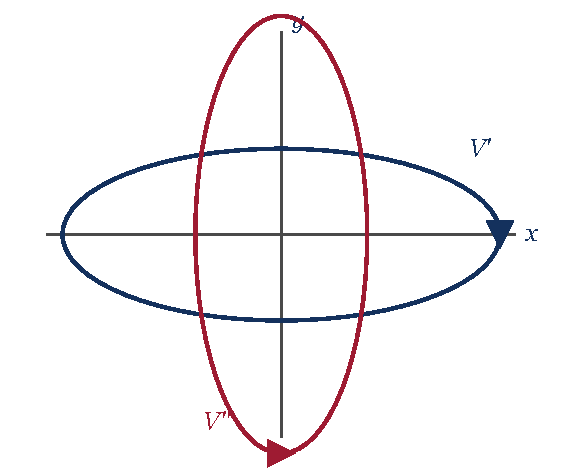
\includegraphics[width=0.5\textwidth]{figuras/pdf/cap06-fig7.pdf}
\caption{Las dos elipses de polarización, iguales y de ejes
perpendiculares, descritas en sentidos contrarios por la molécula
vibrante de los dos rayos refractados en un cristal hemiedro.}
\label{fig:cap6-7}
\end{figure}
